\documentclass[11pt, a4paper,onecolumn, twoside,french]{report}
% openany -> for drafts
\usepackage[a4paper,top=2.5cm,bottom=2.5cm,inner=2.5cm,outer=2.5cm,marginparwidth=2cm,marginparsep=0.05cm]{geometry}
%showframe -> to show the margins and everything
\usepackage[english]{babel}
\usepackage[utf8]{inputenc}
\usepackage[T1]{fontenc}
\usepackage{indentfirst} % alinea on paragraphs
\usepackage[babel=true]{csquotes}
\usepackage{graphicx}
\usepackage[]{amsmath} % fleqn = align blocs on the left
\usepackage{siunitx} % SI units
\usepackage{amssymb} % for convolution sign
%\usepackage{moreverb} % for c, cpp snippets
\usepackage{enumitem} % \begin{enumerate} for more indent in itemize

%\usepackage[english,boxed,lined,onelanguage]{algorithm2e}
%\SetAlCapSkip{1em} % Margin between algo and caption
%\SetAlCapNameSty{textit} % text style for  algo captions
\usepackage{algpseudocode,algorithm,algorithmicx}


\usepackage[acronym,toc,shortcuts]{glossaries}
\usepackage{relsize}



\usepackage{gitinfo2}



\usepackage[toc,page]{appendix}
\usepackage[nottoc,numbib]{tocbibind} % Make the bibliography appear in Summary
\usepackage{fancyhdr} % For titlepage \lhead, \rhead... 
\usepackage[backend=biber,style=ieee-alphabetic,date=long,language=english]{biblatex}
\DeclareFieldFormat*{citetitle}{{\it #1}}
\bibliography{master-thesis.bib}

% To suppress fields in my .bib, try 
% \clearfield, \clearname or \clearlist
% For url date and date, use \DeclareSourcemap
\AtEveryBibitem{\clearfield{doi}}
\AtEveryBibitem{\clearfield{issn}}
\AtEveryBibitem{\clearfield{url}}

\DeclareSourcemap{
  \maps[datatype=bibtex]{
    \map[overwrite=true]{
      \step[fieldset=urldate, null]
    }
  }
}
\usepackage[makeroom]{cancel} % for "crossing" an equation

\usepackage{placeins} % \FloatBarrier for preventing figures to be placed too far away


\def\keywords{\vspace{1em}
{{\it \bf Keywords}:\,\relax%
}}
\def\endkeywords{\par}

\newenvironment{foreword}[1][Foreword]{
	\begin{center}% 
		{\bfseries #1}%
	\end{center}%
}{}


%\usepackage{multirow} % Pour colonnes multiples des tableaux
%\usepackage{longtable} % Pour longs tableaux
%\usepackage{array} % Pour \texttt sur tout une colonne
%\usepackage{xcolor} % Pour éviter que footnote ne bug...
%\usepackage{footnote} % Pour les footnotes dans les tableaux
%\makesavenoteenv{tabular} % Pour les footnotes dans les tableaux
%\usepackage{tabularx}
%\usepackage{pdfpages} % Include des pdfs
%\usepackage[nottoc,numbib]{tocbibind} % Pour faire apparaitre la biblio. dans le sommaire
\usepackage{booktabs} 
\usepackage[font={it}]{caption,subcaption}

\usepackage{color} % For \textcolor

\usepackage{mathtools} % for \shortintertext{} in align block

%\usepackage[]{minitoc} % Intermediate 
\usepackage{etoolbox} % For toggle function (to hide t itlepage)
\usepackage{nth} % 1st, 3rd, 4th...
\usepackage{bm} % \bm{} for bold font in text and math modes
\usepackage[colorinlistoftodos,prependcaption,textsize=scriptsize]{todonotes} %,textsize=tiny
\usepackage[pdfusetitle]{hyperref} % for linkable refs and title in pdf meta
\usepackage[english,capitalise]{cleveref} % capitalise = Fig. instead of fig.

\hypersetup{
    pdfauthor={Maël Valais, François Malgouyres, Jean-Yves Tourneret, Herwig Wendt},%
    %pdftitle={},%
    pdfsubject={This master’s thesis presents the algorithm OMP-PALMTREE for optimizing fast dictionaries using the convolutional tree model},%
    pdfkeywords={deep learning, dictionary learning, sparse image representation, non-convex optimization, machine learning, image processing},%
    pdfcreator={pdfLaTeX (document version: \gitFirstTagDescribe{})},%
    pdfinfo={
        GitVersion={\gitFirstTagDescribe{}}
    } %\gitAbbrevHash
}


\makeglossary
\makeindex



  % <-- all the \usepackages
\fancypagestyle{titlepage}{% 
	\lhead{
\includegraphics[width=0.30\textwidth]{logos/logo-enseeiht.png}}
	\rhead{
\includegraphics[width=0.30\textwidth]{logos/logo-imt.jpg}}
	\lfoot{
\includegraphics[width=0.28\textwidth]{logos/logo-univ-ups.png}}
	\rfoot{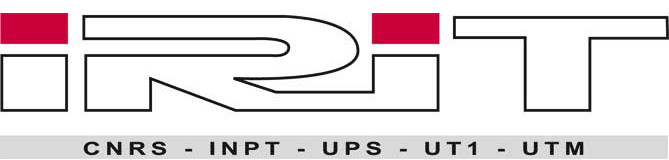
\includegraphics[width=0.28\textwidth]{logos/logo-irit.jpg}}
	\fancyhead[C]{} % On enlève les informations du header
	\fancyfoot[C]{} % On enlève les informations du footer
	\renewcommand{\headrulewidth}{0pt} % On enlève la ligne du header
} \Huge
\fancypagestyle{body}{%
	\restoregeometry 
	\pagestyle{fancy}
	\fancyhf{}
	\fancyhead[LO]{\ifthenelse{\equal{\value{chapter}}{0}}{}{\thesection. \rightmark}} %rightmark = section
	\fancyhead[RE]{\ifthenelse{\equal{\value{chapter}}{0}}
		{}
		{\textsc{Chapter} \thechapter.}
		\textsc{\leftmark}
	} %leftmark = chapter
	\fancyhead[RO]{\thepage} %
	\fancyhead[LE]{\thepage} %
	\renewcommand*{\chaptermark}[1]{\markboth{##1}{}}
	\renewcommand*{\sectionmark}[1]{\markright{##1}{}}
	\renewcommand\headrulewidth{.1pt}
	\setlength{\parskip}{0.2cm} % Espace entre paragraphes
%	\renewcommand{\arraystretch}{1.5} % Espace entre cases d'un tableau
}
\fancypagestyle{plain}{
	\pagestyle{body}
	\fancyhead[LO]{\rightmark}
}
\fancypagestyle{appendix}{%
	\restoregeometry
	% On nettoie les headers et footers existants de "fancy"
	\fancyhf{}
	% Pour le header
	\fancyhead[RE]{Appendix}
	\fancyhead[LO]{\thechapter. \leftmark} %leftmark = chapter
	\fancyhead[RO]{\thepage} %
	\fancyhead[LE]{\thepage} %
	\renewcommand*{\chaptermark}[1]{\markboth{##1}{}}
	\renewcommand\headrulewidth{.1pt}
	% Pour le footer
	%\fancyfoot[C]{\thepage}
	\renewcommand\footrulewidth{0pt}
} % <-- \pagestyle{body}
% MACROS

% Couleurs pour les corrections
\newcommand {\JY}[1] {\textcolor{red}{#1}}
\newcommand {\FR}[1] {\textcolor[rgb]{0.0,0.3,0.0}{#1}}
\newcommand {\OL}[1] {\textcolor{blue}{#1}}
\newcommand {\HW}[1] {\textcolor[rgb]{0.3,0.2,0.0}{#1}}
%\newcommand{\hilite}[1] {\emph{#1}}
\newcommand{\hilite}[1] {\Req{#1}}
\newcommand {\Req}[1] {\textcolor[rgb]{0.75,0.0,0.0}{#1}}
\newcommand {\Geq}[1] {\textcolor[rgb]{0.0,0.5,0.0}{#1}}
\newcommand {\Beq}[1] {\textcolor[rgb]{0.0,0.15,0.60}{#1}}
\newcommand {\black}[1] {\textcolor{black}{#1}}

% Espaces mathématiques
\newcommand {\DPUN} {{\mathcal D}}
\newcommand {\DTREE} {{\mathcal D}^e}
\newcommand {\CC} {\mathbb C}
\newcommand {\RR} {\mathbb R}
\newcommand {\RP} {\mathbb R^{\mathcal P}}
\newcommand {\RPE} {\mathbb R^{\mathcal P \times |\edges |}}
\newcommand {\codeset} {\mathbb R^{\mathcal P \times \leaves}}
\newcommand {\Dset} {\mathbb R^{\mathcal P \times (\mathcal P \#\leaves) }}
\newcommand {\ZZ} {\mathbb Z}
\newcommand {\NN} {\mathbb N}
\newcommand {\PP} {{\mathcal P}}
\newcommand {\HH} {{\mathbb H}}
\newcommand {\II} {{\mathbb I}}
\renewcommand {\SS} {{\mathcal S}} % applis supports
\newcommand {\SA} {{\mathbb S}} % support accessible

% Fonctions
\newcommand {\f}[1] { {\mathcal F}\left( #1 \right) }
\newcommand {\F}[1] { {\mathcal F^{-1}}\left( #1 \right) }
\newcommand {\norm}[2] {\left\| #1 \right\| _{#2}}
\newcommand {\defeq} {\triangleq}

% Opérateurs
\DeclareMathOperator {\sign} {sign}
\DeclareMathOperator {\prox} {prox}
\DeclareMathOperator {\argmin} {argmin}
\DeclareMathOperator {\supp} {supp}
\DeclareMathOperator {\rg} {rg}
\DeclareMathOperator {\diag} {diag}
\newcommand {\RG}[1] {\rg\left( #1 \right)}
\newcommand {\SUPP}[1] {\supp\left( #1 \right)}
\newcommand {\PS}[2] {\langle #1 , #2 \rangle}
\newcommand {\PROBA}[1] {\mathbb P \left( #1 \right)}
\newcommand {\one}[1] {\mathbbm{1}_{ #1 }}
%\newcommand {\one}[1] {\chi_{ #1 }} %{\mathbbm{1}_{ #1 }}
\newcommand {\oneinf}[1] {\chi_{ #1 }}
%\newcommand {\oneinf}[1] {{\mathcal I}_{ #1 }} 

% Acronymes
\newcommand {\PSNR} { \textrm{PSNR}^* } 
\newcommand {\NRE} { \textrm{NRE} }
\newcommand {\CPR} { \textrm{RER} }
\newcommand {\COST} { \textrm{G} } % ancien compression ratio

% Raccourcis
\newtheorem{prop}{Proposition}[section]

\newcommand {\nodes} {\mathcal N}
\newcommand {\edges} {\mathcal E}
\newcommand {\leaves} {\mathcal L}
\newcommand {\NL} {\#\leaves}
\newcommand {\hall} {h^e _{e \in \edges}}
%\newcommand {\multiconv}[1] { \bigstar_{\substack{#1}}\, }
\newcommand {\multiconv}[1] { \mathbf h^{#1}\, }
\newcommand {\tpath}[1] {\mathcal{C}(#1)}
\newcommand {\code} {\mathbf x}
\newcommand {\data} {\mathbf y}
\newcommand {\dataex} {\mathbf b}
\newcommand {\databis} {\mathbf y^e}
\newcommand {\D} {\mathbf D}
\newcommand {\Hs} {\mathbf A}
\newcommand {\Ha} {\mathbf H}
\newcommand {\Haf} {\hat{\mathbf H}}
\newcommand {\Hab} {\bar{\mathbf H}}
\newcommand {\res} {\mathbf r}

\newcommand {\tree}{\mathcal T}
\newcommand{\subtree}[1]{\tree^{#1}}

\newcommand {\stopalgo}{\epsilon}

% autres MACROS
\newcommand {\hkall} {(h^k)_{1 \leq k \leq K}}
\newcommand {\hkconv} {h^1 * \dots * h^K}
\newcommand {\hkconvnorm} {\frac{h^1}{\norm{h^1}{2}} * \dots * \frac{h^K}{\norm{h^K}{2}}}
\newcommand {\hkconvp} {g^{1} * \dots * g{K}}
\newcommand {\hkconvs} {f^{1} * \dots * f^{K}}
\newcommand {\fobj} {\| \code * h^1 * \dots * h^K - \data \|_2^2}
\newcommand {\fobjlambda} {\| \lambda \code * h^1 * \dots * h^K - \data \|_2^2}

% Macros added by Mael
\newcommand{\file}{\texttt}
\newcommand{\dispCode}{\texttt}
\newcommand{\dispCodeLong}[1]{
\begin{verbatim} #1 \end{verbatim}
}
\DeclareMathOperator*{\argmax}{\arg\!\max}% http://tex.stackexchange.com/q/83169/5764

\algnewcommand\algorithmicinput{\textbf{Input:}}
\algnewcommand\Input{\item[\algorithmicinput]}
\algnewcommand\algorithmicoutput{\textbf{Output:}}
\algnewcommand\Output{\item[\algorithmicoutput]}    % <-- \x, \y, \D...
% \newacronymwithdescr{Label}{Court}{Long}{Description}
\newcommand*{\newacronymwithdescr}[5][]{%
  \newglossaryentry{main-#2}{name={#3},%
  text={(\acs{#2}) #3\glsadd{#2}},%
  description={#5},%
  #1
  }%
  \newacronym{#2}{#3\glsadd{main-#2}}{#4}%
}

% Pas de point final pour les entrées glossaire ou acronymes
\setacronymstyle{sm-short-long}
%\newacronym{IMT}{IMT}{Institut de Mathématiques de Toulouse}
\newacronymwithdescr{IMT}{IMT}{Institut de Mathématiques de Toulouse}{is the main laboratory in mathematics in Toulouse}
\newglossaryentry{Blabla}{name=Blabla,description={is....}}

% To use the glossary entries:
% \acs{} (for short one)
% \ac{} (for long one - only on first appearence)

  % <-- acronyms (\ac{PALM}...)
\author{Maël Valais}
\date{Updated on \today}
\title{Optimization of dictionaries structured in convolutional trees for sparse image representation - Master’s Thesis}
\begin{document}
\begin{titlepage}
\thispagestyle{pagedegarde}
\newgeometry{tmargin=2.2cm,bmargin=4cm,lmargin=2cm,rmargin=2cm}
\begin{center}
\topskip2.8cm
\textsc{Université Toulouse III — Paul Sabatier}\\
\vspace{0.5 cm}
\line(1,0){100}\\
\vspace{0.6 cm}
{{{Internship Report}}}\\
\vspace{0.3cm}
Defended on September 15\th, 2016\\ \vspace{0.3 cm} par\\ \vspace{0.3 cm} \textbf{Maël \textsc{Valais}}\\
\vfill
{\Huge \textbf{Optimization of dictionaries structured as convolutions trees for sparse image representation }}\\
\vfill

{{Internship at \acs{IMT}}}\\
{Université Paul Sabatier}\\
{118, route de Narbonne}\\
{31400 Toulouse}\\
\vspace{2 cm}

\par Supervised by \\ \textbf{François \textsc{Malgouyres}}\\
Institut de Mathématiques de Toulouse\\ 
%\vspace{1cm}
\par and \\Jean-Yves \textbf{ \textsc{Tourneret}}\\
ENSEIHHT, Toulouse
\end{center}
\end{titlepage}

% Préparation pour les pages de corps
\pagestyle{empty}
\restoregeometry
\cleardoublepage % Blanc jusqu'à prochaîne page paire

\tableofcontents
{\let\clearpage\relax\listoffigures}
{\let\clearpage\relax\listoftables}
{\let\clearpage\relax\listofalgorithms}

\pagestyle{corps} % Uncomment to show title page
\pagestyle{empty} \restoregeometry
%\cleardoublepage % White until the next even page
\pagestyle{body}
%\abstract{} \todo[inline]{Write an abstract}
%{\centering \subsection*{Foreword}} \addcontentsline{toc}{subsection}{Foreword}\todo[inline]{Write a foreword}
\tableofcontents
%{\let\clearpage\relax\listoffigures}
%{\let\clearpage\relax\listoftables}
%{\let\clearpage\relax\listofalgorithms}



\chapter{Introduction} %\markboth{Introduction}{}}

\section{The need for sparse representations}

A sparse signal over some representation means that it can be expressed using only a few elements of the representation – in other words, sparse means with many zeros. Many applications ranging from machine learning to image denoising and image recognition heavily rely on the property that we can summarize (or more exactly approximate) any signal using a proper sparse representation. The job of obtaining the raw\footnote{A “raw” signal is represented in the canonical basis} signal from its sparse counterpart can be written in terms of an operator, often called \emph{dictionary} or \emph{transform}.

This chapter will review the main existing dictionaries that have been used for sparse representation, from non-adaptative transforms to learned dictionaries and through the intermediate over-complete dictionaries.

\section{Basis and redundant dictionaries}

The \ac{DFT} is a classical example of operators used for sparsity. The \ac{DFT} can be written as a matrix $\D$, where $\D$ denotes the dictionary. Finding the Fourier representation – which we will refer as the \emph{code} $\x$ – of an image $\y$ amounts to compute 
$$\x = \D^T\y.$$

\begin{figure}[!ht]
\subcaptionbox{Picture $\y$ with many discontinuities.}%
  [.49\linewidth]{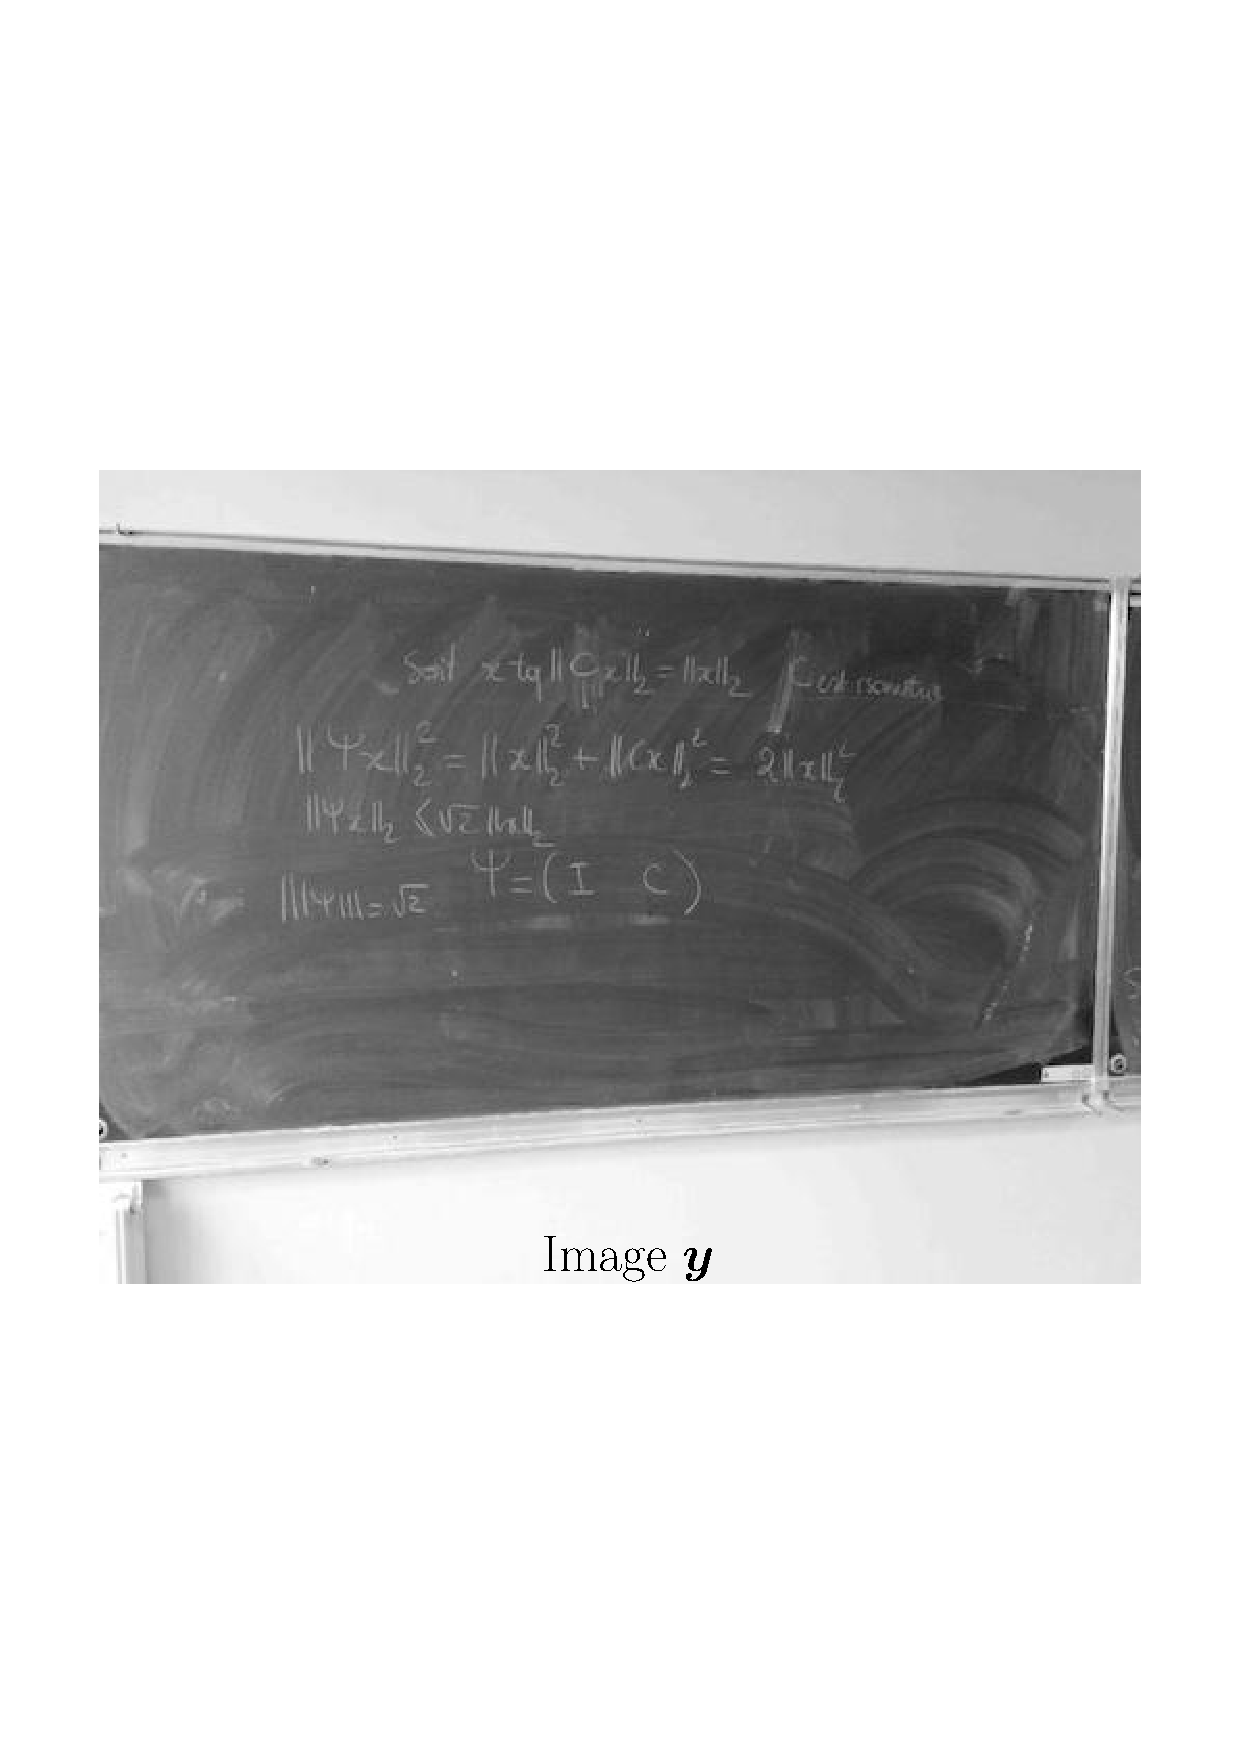
\includegraphics[width=0.49\textwidth]{figures/fourier/image.pdf}}
 \subcaptionbox{Result of applying the Fourier transform to $\y$}%
  [.49\linewidth]{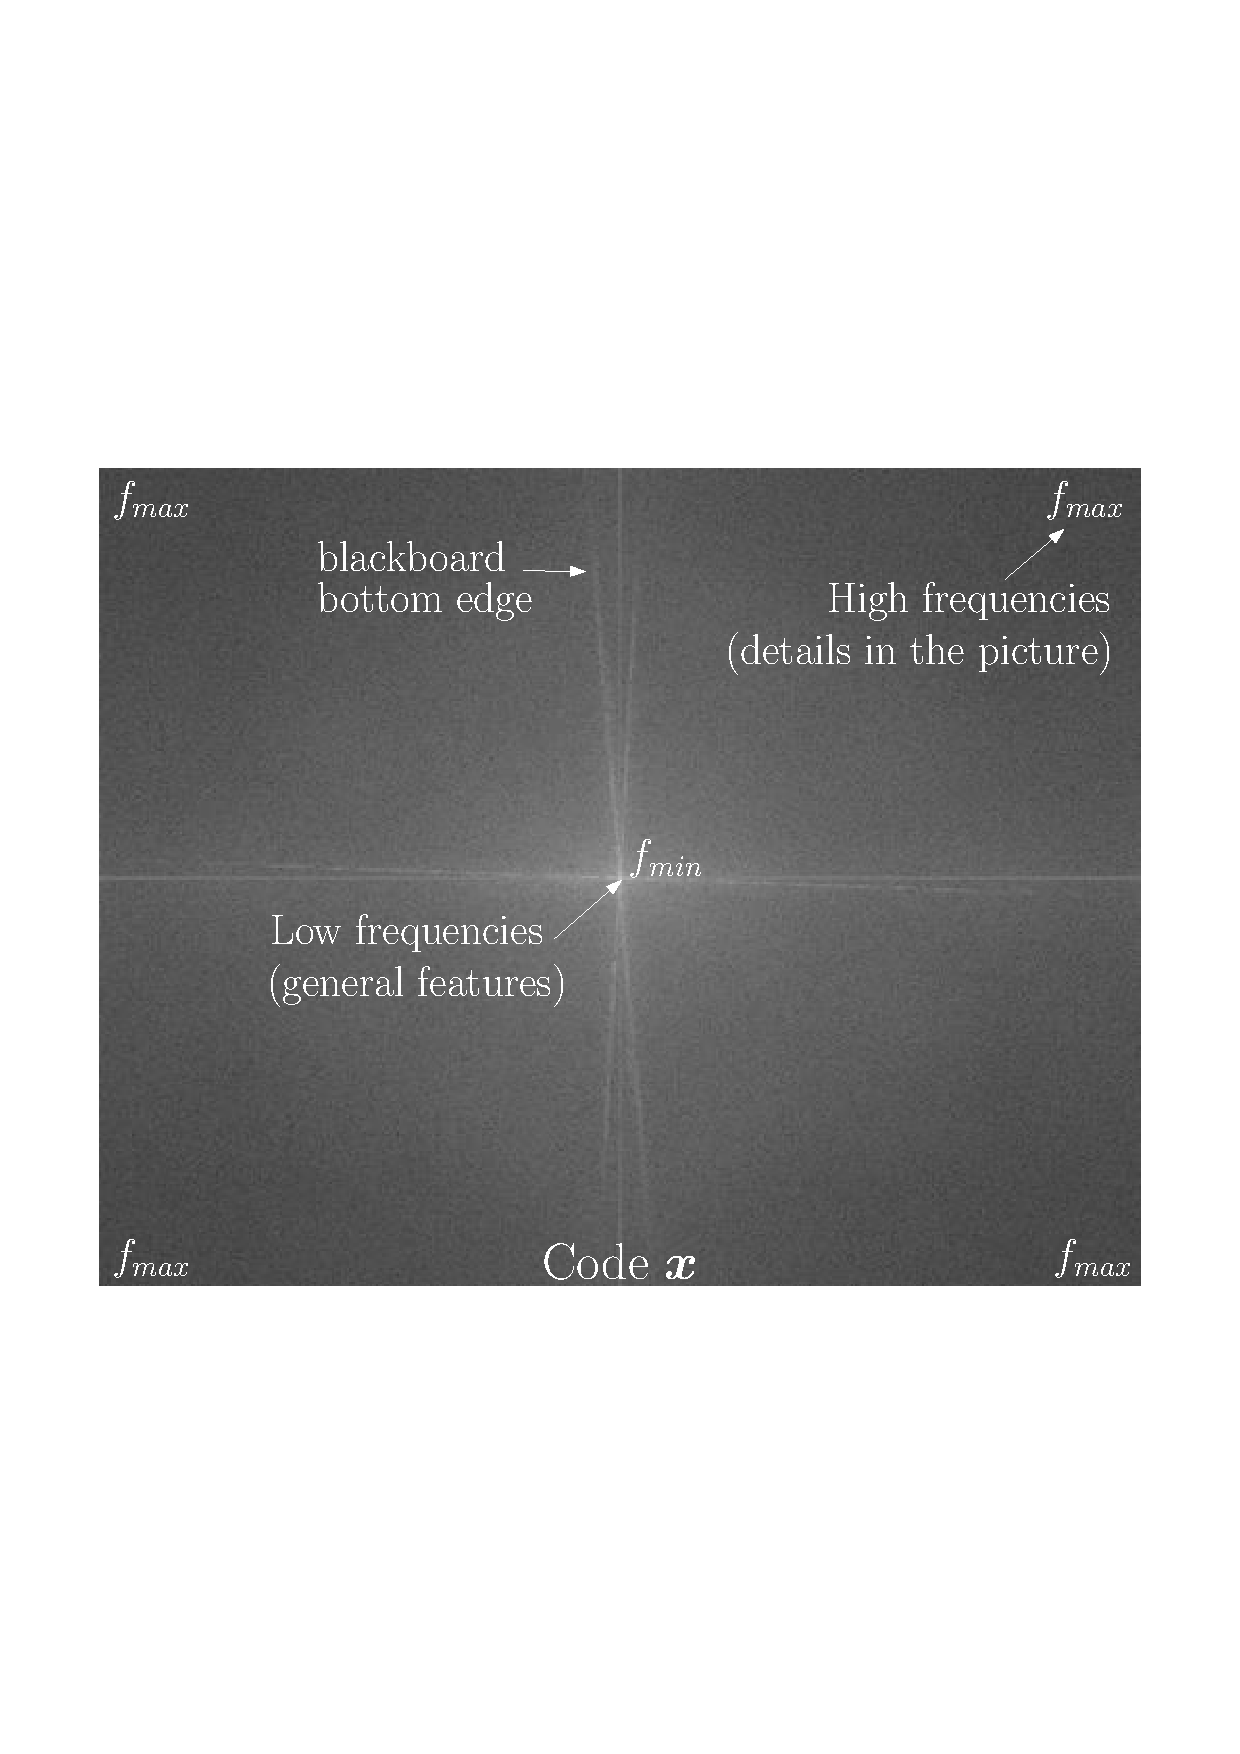
\includegraphics[width=0.49\textwidth]{figures/fourier/fourier.pdf}}
  \caption{Decomposition $\D^T\y=\x$ of a signal $\y$ using the dictionary $\D$ made of Fourier series. In $\x$, the middle coefficients are coding “large” features while the corner values are coding the details. The multiple white lines, ranging from the middle to the borders, outline the discontinuities caused by the blackboard edges; these coefficients are scattered (hence not sparse), which shows that the Fourier basis has representation problems in presence of discontinuities.} \label{fig_fourier}
\end{figure}

However, the Fourier transform is quite different from the representations we have in mind, namely the convolutional tree structure. First, Fourier forms a basis, implying that it is a one-to-one representation in the sense that every code $\x$ is associated with a unique image $\y$. This basis is also orthogonal, meaning that the operator is stable (it does not amplify errors). \todo{The basis is normed, meaning what?}

More importantly, the \ac{DFT} has interesting properties that allow fast implementations. For example, applying the Matlab function \texttt{fft2} to the \cref{fig_fourier} takes less than a millisecond. If we assume $N$ to be the dimension of the concatenated\footnotemark[2] image, instead of computing a time-expensive $O(N^2)$ matrix-vector product, the fast Fourier transform only requires a computational cost of the order $O(N \log N)$.

\footnotetext[2]{Also referred as “vectorized”; we consider 2-D images as one-dimensional vectors. A $16 \times 16$ image would give a vector of dimension 256.}


The Fourier transform is widely used as an operator for sparse representations, mainly when dealing with smooth signals that can be approximated by a sum of sinusoids. However, this operator does not generally perform well on images since they contain many discontinuities that are far from being representable using sinusoids.

The problem with discontinuities is illustrated in \cref{fig_fourier}. As an example, the bottom edge of the blackboard (which is a strong discontinuity) induces a long vertical trail of high coefficients in $\x$. Because of discontinuities, $\x$ is forced to have many non-zero coefficients. 

Along with Fourier, many other basis dictionaries exist; we can mention the cosine transform which is at the core of JPEG compression. We can also cite the wavelet transform, used in JPEG2000 compression. Note that both wavelets and cosine are stable and have fast implementations.

\section{Redundant dictionaries}

Basis dictionaries were generalized by using multiple bases to form a stable and redundant (also called over-complete) dictionary in \cite{chen_atomic_2001}. For example, combining a canonical basis with a cosine basis would allow both peaks and sinusoids to be represented.

Other redundant dictionaries, like the curvelet transform, do not rely the useful properties of bases, yet being stable and having a fast implementation. It is interesting to note that unlike Fourier or cosine transforms, the curvelets can code (to an extent) non-smooth signals.

% Notes for myself
% 1. tight frame = preserves the norm
% 2. orthogonality preserves the norm (norm doesn’t make the errors explode)
% 3. orthogonal means that it is stable

Although offering excellent performances for sparse representation thanks to the fast implementations, redundant dictionaries still lack adaptativity.


\section{Learned dictionaries}
Previously mentioned dictionaries are said to be “non-adaptative”, meaning that they won’t be able to sparsely code every possible type of signal.

Dictionary learning allows to create “adaptative” dictionaries. Instead of being fixed, atoms are based on a learning set of example images, denoted by
$$\Y = \begin{bmatrix} \y_1 & \dots & \y_S \end{bmatrix}$$
where the columns of $\Y$ are the vectorized\footnote{A vectorized matrix of dimension $I \times J$ of an image is the concatenation of all columns to form a vector of size $IJ$} images $\y_i$ of dimension $N$. The dictionary $\D$ is made of $K$ columns $\d_i$ (the atoms) such that the number of atoms is much larger than the dimension of a single image $\y_i$ ($K \gg N$):
$$\D = \begin{bmatrix} \d_1 & \dots & \d_K \end{bmatrix}.$$

The codes $\X$ are defined by
$$\X = \begin{bmatrix} \x_1 & \dots & \x_S \end{bmatrix}$$
where $\X$ is the concatenation of $S$ column vectors $\x_i$ (the codes) of dimension $K$. The dictionary learning problem is defined as
\begin{align}
\underset{\D,\X}{\min}~ & \lVert \X \rVert_1 + \lambda\lVert \D\X-\Y \rVert^2_F \tag{$DL$} \label{eq_dl} \\
\text{s.t.}~ & \lVert \d_k \rVert \le \gamma & \forall k = 1,\dots,K\label{eq_dl_finite_norm}
\end{align}
where $\lVert . \rVert_F$ denotes the Frobenius norm and $\lVert . \rVert_1$ is the $l_1$ norm defined by $\lVert \X \rVert_1 = \sum_{i=1}^S |\x_i|$. The constraint \ref{eq_dl_finite_norm} prevents the atoms from having an arbitrarily big norm.

The problem \eqref{eq_dl} can be understood as finding the atoms of $\D$ that give the sparsest (with as many zeros as possible) representation $\x_i$ approximating $\y_i$ for all $i = 1,\dots,S$. This approximation is denoted
$$\D\X \approx \Y$$

\Cref{fig_overcomplete_matrix} gives an idea of what we mean by approximating an image $\y$ using the matrix-vector product of a sparse code $\x$ and a learned dictionary $\D$. For this example, $\y$ is represented by a linear combination of three atoms of $\D$: $\x$ is 3-sparse.

\begin{figure}[!ht] \centering
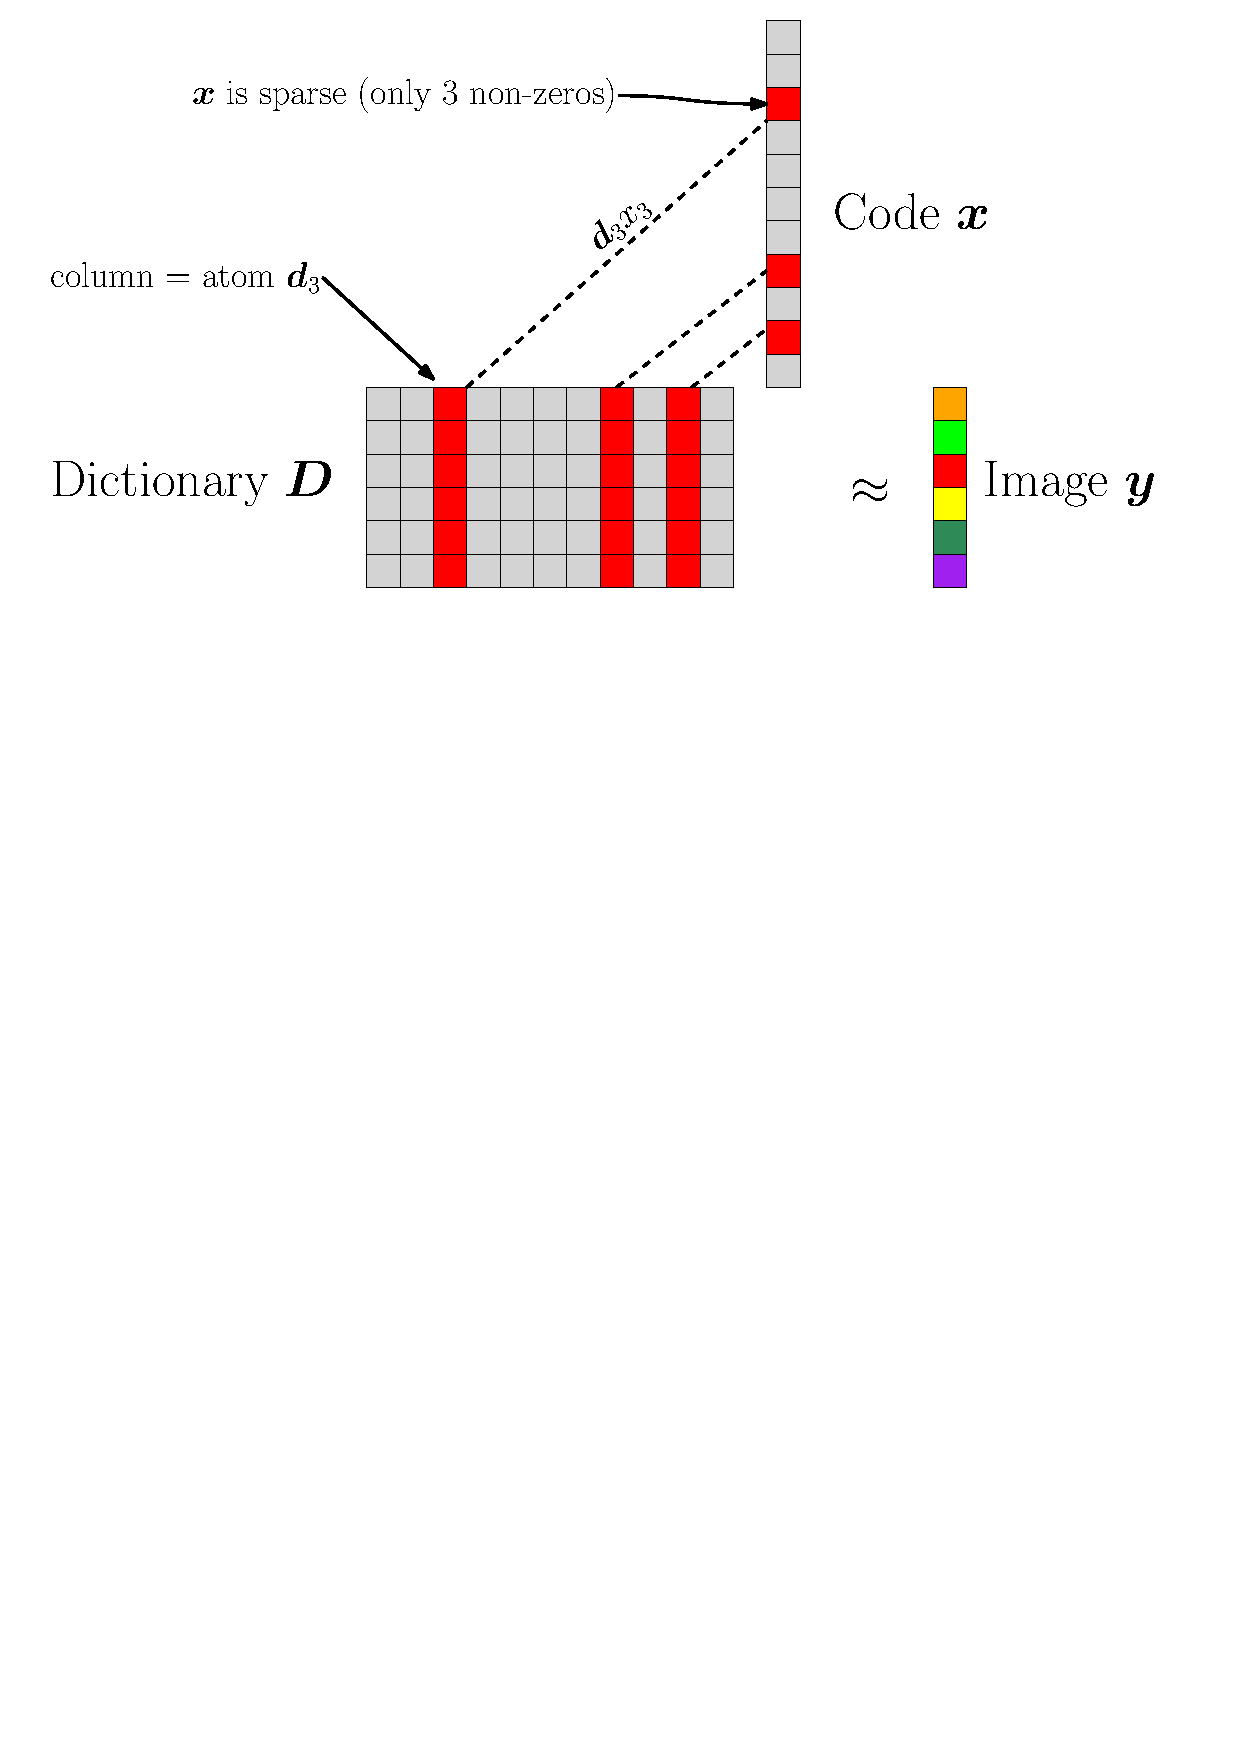
\includegraphics[width=0.80\textwidth]{figures/sparsity-matrix.pdf}
\caption{Matrix view of $\D\x$ when $\D$ is over-complete (much more columns than lines).}\label{fig_overcomplete_matrix}
\end{figure}


The non-linearity caused by the product $\D\X$ induces a non-convex objective function, making it difficult to optimize simultaneously with respect to $\D$ and $\X$. To work around this problem, many algorithms solving \eqref{eq_dl} alternatively optimize the dictionary $\D$ and the codes $\X$.

\subsection{Existing dictionary learning algorithms}
Among the many available algorithms (and their multiple versions) for dictionary learning, the \ac{KSVD} algorithm is a typical example. Introduced in \cite{aharon_k-svd:_2006} and inspired by the widely known \gls{KMeans} algorithm, it is used in many image processing applications. This algorithm is detailed in the next section.

Another approach, more scalable, is denoted as “online” dictionary learning. The Online Dictionary Learning algorithm, proposed in \cite{mairal_online_2010}, learns one image after the other instead of learning the whole set at once. It makes it very suitable for huge sets of learning images.


\subsection{Example with the \acs{KSVD} algorithm}

Among the many existing alternating algorithms for dictionary learning, the \ac{KSVD} algorithm is well known for its state-of-the-art performance in image denoising. \ac{KSVD} is responsible for many concepts behind the \acs{PALMTREE} algorithm (the algorithm we are trying to improve and developed in \cite{chabiron_optimization_2016}). This section summarizes the key elements of the \ac{KSVD} algorithm.

\ac{KSVD} does not actually solve \eqref{eq_dl}; instead, it gives a solution for a “stronger” problem in the sense that the level of sparsity in \ac{KSVD} is enforced by $\gamma$ in
\begin{align*}
\underset{\D,\X}{\min}~ & \lVert \D\X-\Y \rVert^2_F \tag{$DL_2$}\label{eq_dl_ksvd} \\
s.t.~& \lVert \x_i \rVert_0 \le \gamma \quad \forall i \text{ in } 1,\dots,S
\end{align*}
where $\lVert . \rVert_F$ denotes the Frobenius norm and $\lVert . \rVert_0$ is the pseudo-norm $l_0$ (also known as “counting function”).

The \emph{Sparse Coding step} optimizes with respect to $\x$; this step basically uses \ac{OMP} (see \cref{alg_omp}) or any other pursuit algorithm. The \emph{Dictionary Update step} optimizes w.r.t. $\D$. This is the step that was studied in \cite{chabiron_optimization_2016}. Note that the full \ac{KSVD} algorithm is presented in \cref{sec_ksvd_detail}, \cpageref{sec_ksvd_detail}.

\Cref{fig_ksvd} gives an example of what “learning $\D$” means with the \ac{KSVD} algorithm. As the image (a) is too big ($512 \times 512$) to be learned directly, we must chop it into many small patches of size $16 \times 16$. (b) shows some of these patches contained in $\Y$, which actually holds 10240 patches ($\Y$ has dimension $128 \times 10240$). The dictionary $\D$ of size $128 \times 128$ (it has 128 atoms) is shown in (c). $\D$ has been learned with a sparsity of 10 and the process took about five minutes (stopped after 20 iterations).

The dictionary in (c) can now be used for denoising the noisy image (a). If we wanted a dictionary for image recognition or compression, we would probably use many more images.

\begin{figure}[!ht]\centering
\begin{subfigure}[b]{0.40\textwidth}\centering
	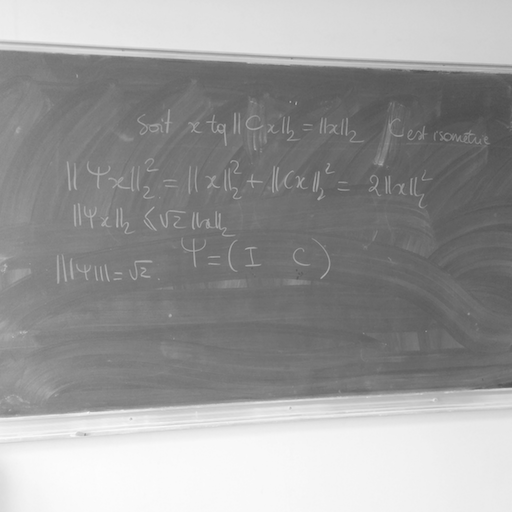
\includegraphics[width=\textwidth]{figures/ksvd/tableau_512x512.png}
	\caption{Image used for learning}
\end{subfigure}
\begin{subfigure}[b]{0.29\textwidth}\centering
	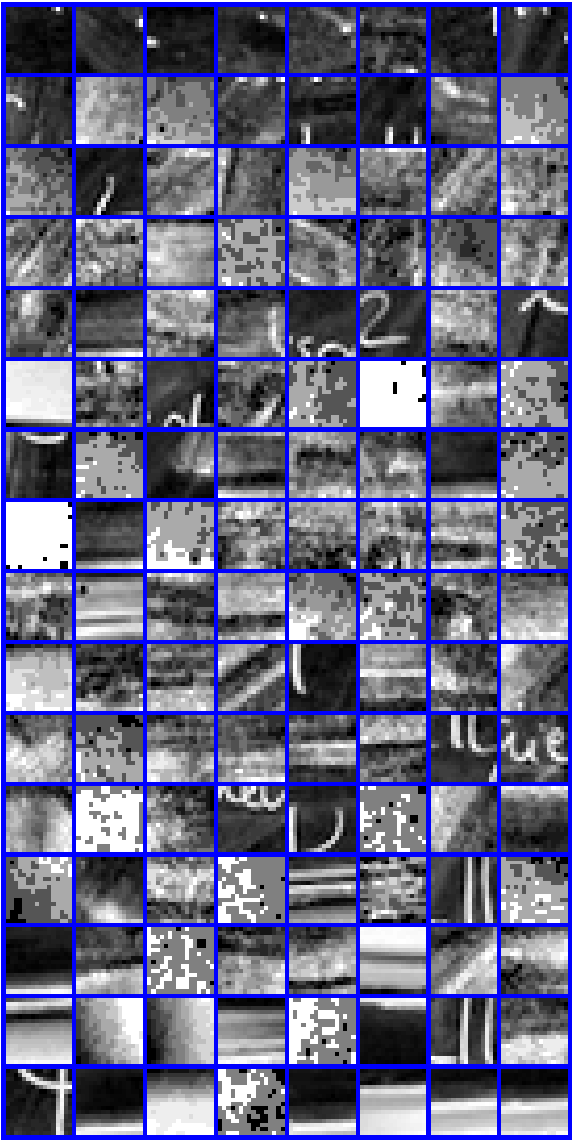
\includegraphics[width=0.7\textwidth]{figures/ksvd/patches.pdf}
	\caption{Image patches $\Y$}
\end{subfigure}
\begin{subfigure}[b]{0.29\textwidth}\centering
	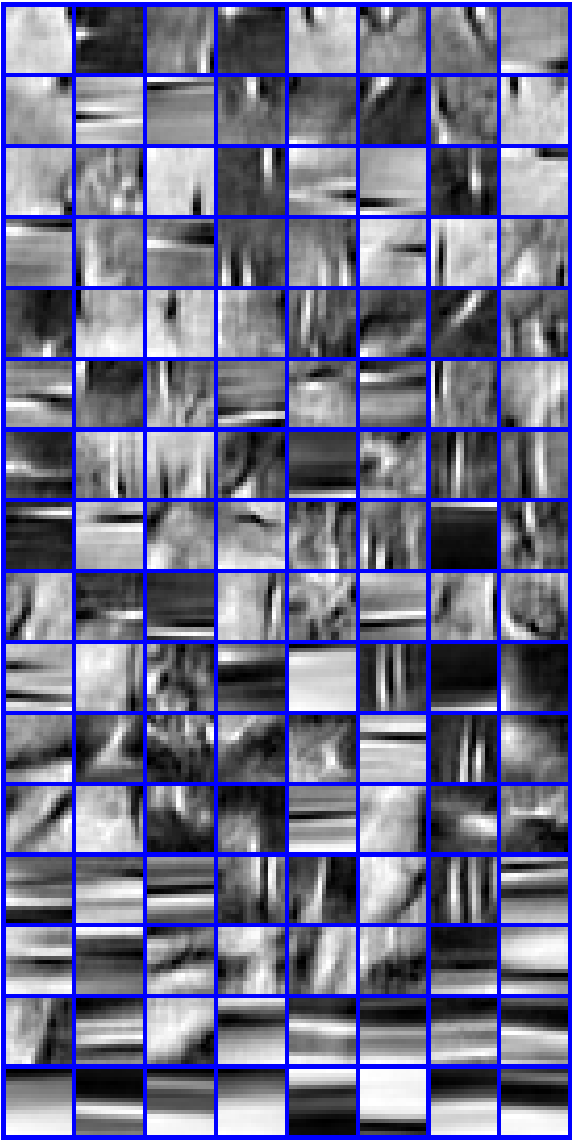
\includegraphics[width=0.7\textwidth]{figures/ksvd/dictionary.pdf}
	\caption{Learned $\D$}\label{fig_ksvd_dict}
\end{subfigure}
\caption{Learning $\D$ on image patches using \ac{KSVD}.}\label{fig_ksvd}
\end{figure}


\subsection{Problem of atom scalability: multi-scale dictionaries}
As the learned \ac{KSVD} dictionary relies on the $O(NK)$ matrix-vector product and has to be over-complete ($K \gg N$) in order to achieve sparsity, we easily understand that $N$ cannot take an arbitrarily large value. In practice, the example images (also called patches) and atoms of the dictionary are generally at most $16 \times 16$.

Dictionaries with bigger atoms are known as multi-resolution (also called multi-scale), meaning that the atoms can contain either details or large features in images.


\subsection{Problem of atom redundancy: convolutional dictionaries} \label{sec_atoms_redund}
The \ac{KSVD} algorithm is not translation-invariant in the sense that multiple atoms of the dictionary can have the same detail but slightly translated. The authors of \cite{mailhe_shift-invariant_2008} worked on making the update step invariant by translation, but it still needs a lot of tuning and finding the right parameters.

Translation-invariant transforms are known as convolutional dictionaries. Instead of many atoms containing translated version of the same feature, convolutional dictionaries contain all possible translations for every atoms; unlike traditional learned dictionaries, it is unlikely to find two atoms containing the same detail with different locations.

Many state-of-the-art machine learning techniques are based on trees of convolutions, like the Convolutional Neural Networks used in Deep learning \cite{lecun_deep_2015}.

\section{Research motivations and objectives}
 The many sparse representation applications are only limited by the performance of their transforms. By performance, we mean that the transform must be
\begin{itemize}
\item[--] fast (fast computation of $\D\x$),
\item[--] adaptative (must be learned on a set of images)
\item[--] and stable.
\end{itemize}

As mentioned, many algorithms are available, but are often fast at the expense of adaptiveness (such as the Fourier transform) or adaptative at the expense of speed (such as \ac{KSVD}).

The main objectives of this work is to develop a multi-resolution (larger atoms) dictionary model that computes fast and is adaptive, based on the principle of convolutional trees. During its PhD thesis, Olivier Chabiron has been working on the \Gls{treemodel}, presented in the article \citetitle{chabiron_optimization_2016} (\cite{chabiron_optimization_2016}). 


\section{Related work}
Two other teams are also actively working on multi-resolution transforms:
\begin{itemize}
	\item[--] the team lead by Mickeal Elad proposed a dictionary model based on wavelets in the article \citetitle{sulam_trainlets:_2016} (cf. \cite{sulam_trainlets:_2016});
	\item[--] Rémi Gribonval’s team has proposed a factorization-based dictionary model in the article \citetitle{magoarou_flexible_2016} (cf. \cite{magoarou_flexible_2016}).
\end{itemize}
Their work have been published very recently (early 2016); this thesis does not detail these papers, but studying these advances will be done right after the end of this internship, during the PhD thesis.

\chapter{State of the art}

\section{Dictionary structured by the \Gls{treemodel}}

\subsection{\Gls{treemodel}}\label{sec_tree_model}
The work studied in \cite{chabiron_toward_2015} and \cite{chabiron_optimization_2016} offers a different way of structuring the matrix $\D$, namely the \emph{\Gls{treemodel}}. Instead of using “plain” atoms as columns and dealing with the matrix-vector product in $O(NK)$, $\D$ is defined by a convolutional tree structure $$\T(\V,\E)$$ where each edge $e$ of $\E$ is characterized by a kernel $\h^e$ and a support $\s^e$. The root $r$ and leaves $l$ of $\V$ allow us to define a branch as the successive edges growing from the root to one of the leaves.

\begin{figure}[!ht]\centering
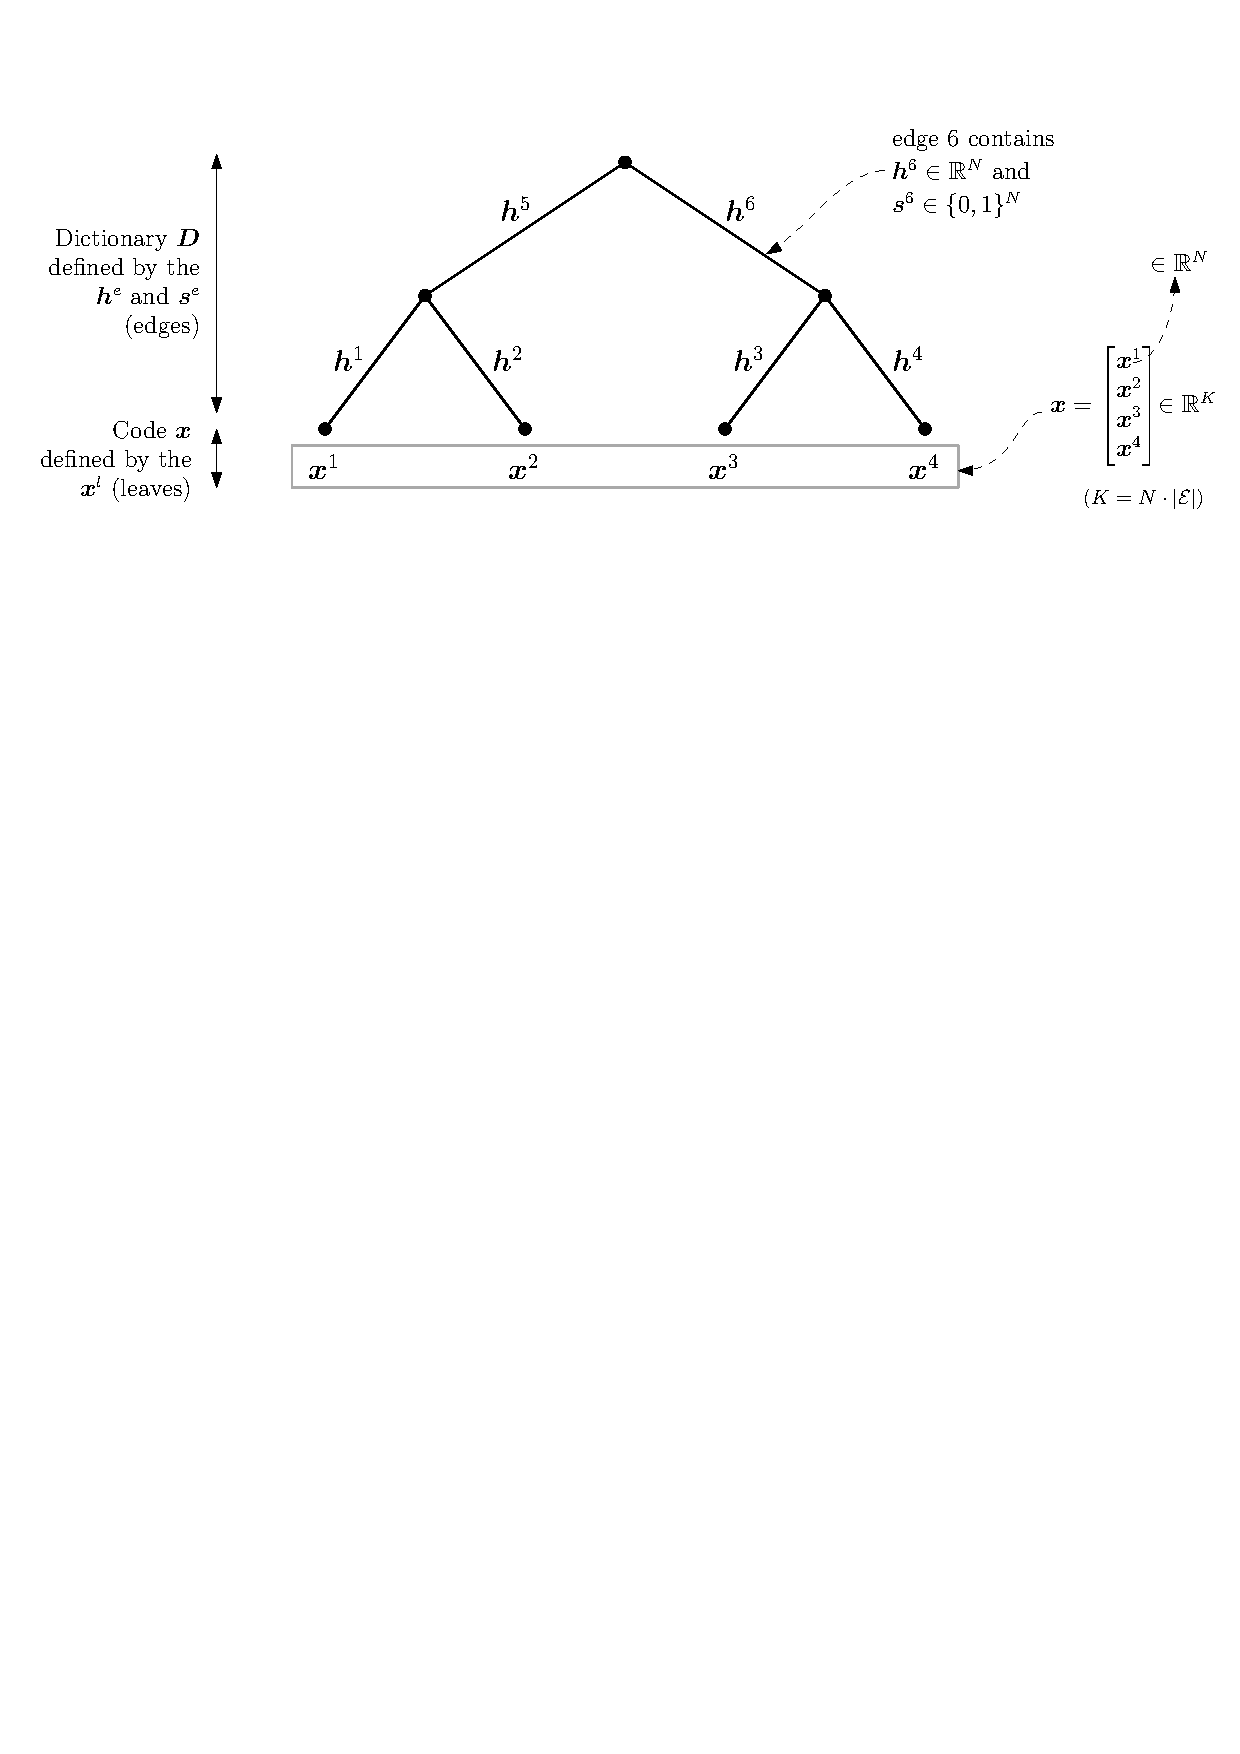
\includegraphics[width=\textwidth]{figures/tree.pdf}
\caption{View of a convolutional tree; the $\h^e$ and $\s^e$ are what define $\D$}\label{fig_tree}
\end{figure}

The target image $\y$ as well as the kernels $\h^e$ and supports $\s^e$ are vectors of dimension $N$. The supports $\s^e$ only take the values 0 (corresponding value in $\h^e$ must be 0) or 1 (corresponding value in $\h^e$ can be non-zero). For easier reading, we will denote the families $(\h^e)_{e \in \E}$ and $(\s^e)_{e \in \E}$ by $$\h = (\h^e)_{e \in \E}$$ and $$\s = (\s^e)_{e \in \E}.$$

The code $\x$ is a “big” vector of dimension $K$ with $K = N \times |\L|$ such that $$\x = \begin{bmatrix}\x^1_1 \\ \vdots \\ \x^{|\L|}_N\end{bmatrix}$$

 $\D$ is a matrix of dimensions $N \times K$ and $\y$ is a vector of dimension $N$.

In the following, we will denote the images interchangeably using the vector notation $y = \{ y_i ~|~ i=1,\dots,N \}$ or the linear map notation $y = \{y(p) ~|~ p \in \P\}$.

The \cref{fig_example_kernel} displays examples of a standard kernel (left) and a kernel $\h^e$ (middle) associated with its support $\s^e$ (right). The gray squares represent the “ones” of the support while the kernel is represented by values.

\begin{figure}[!ht]\centering
\begin{subfigure}[b]{0.20\textwidth}\centering
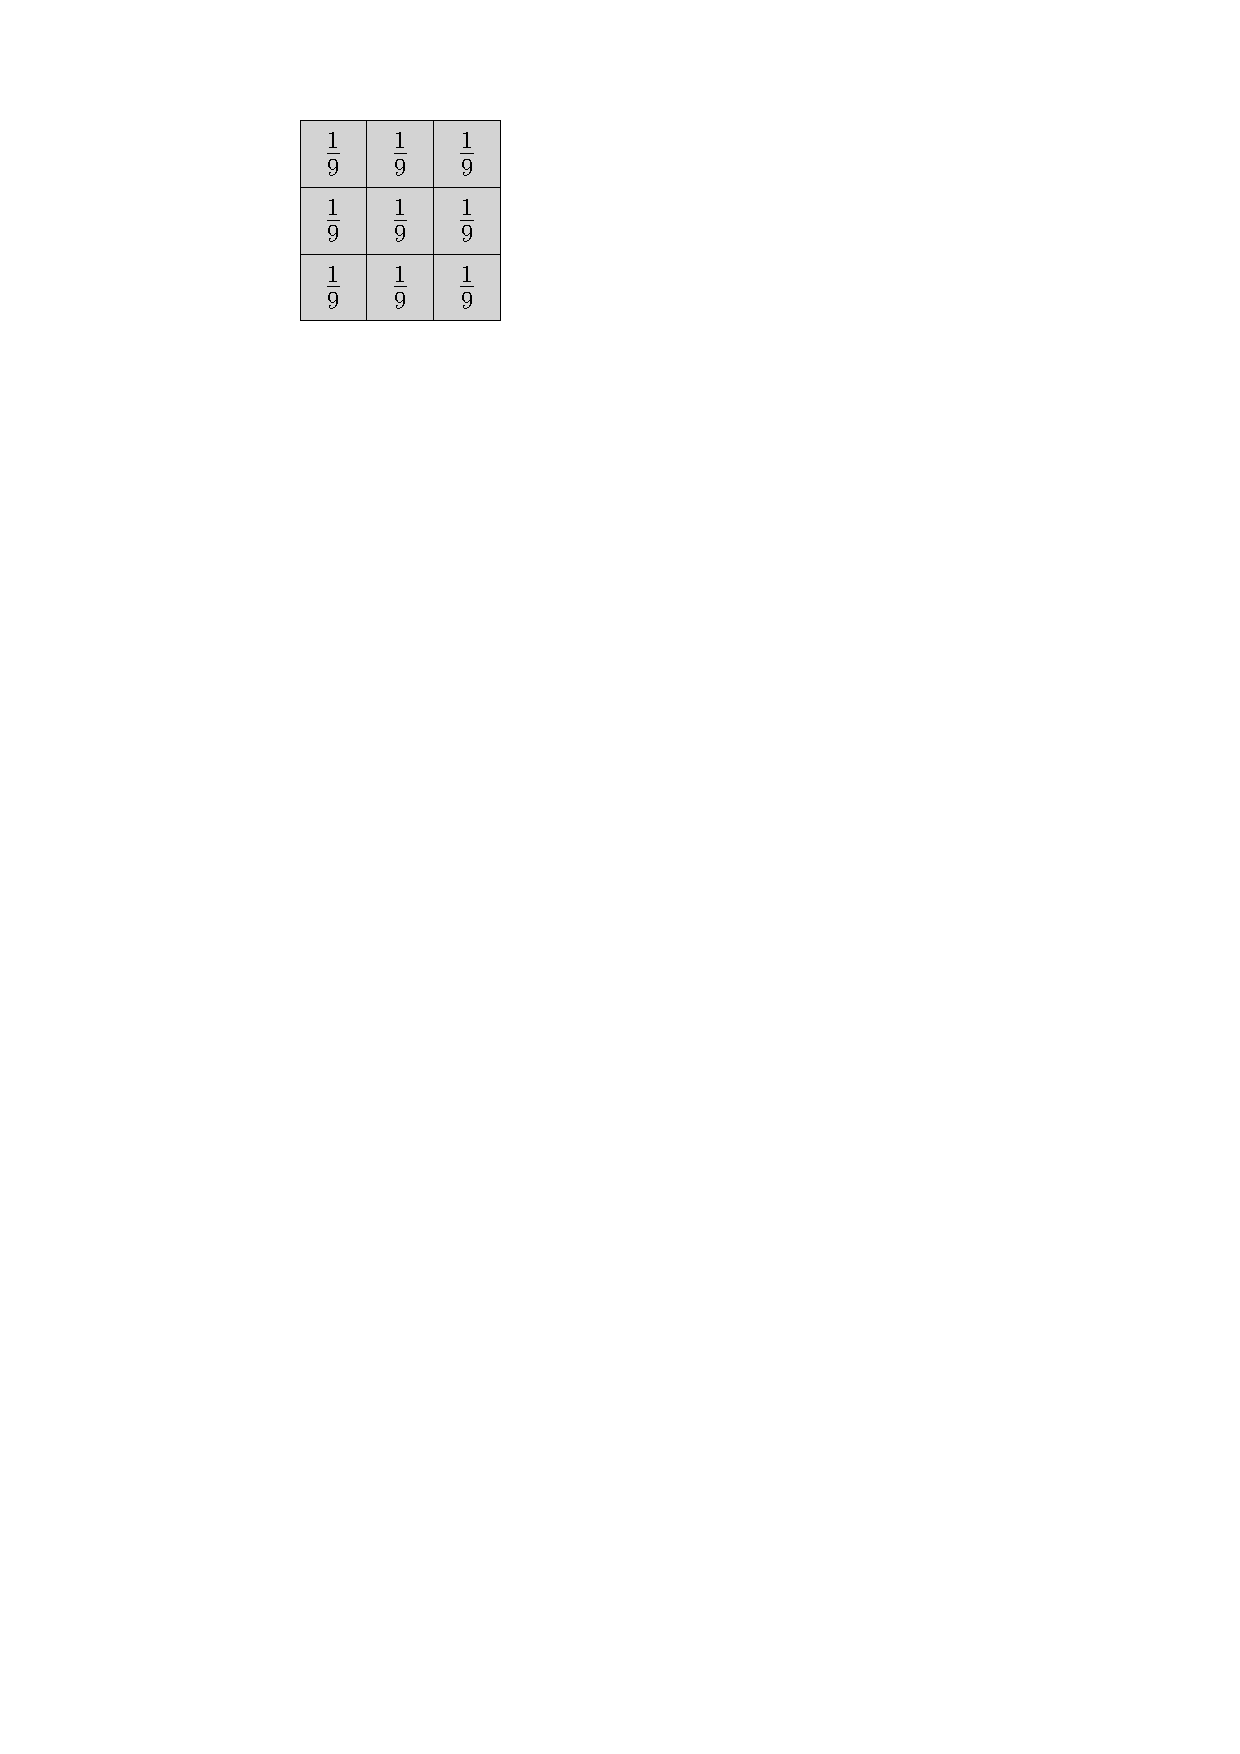
\includegraphics[width=0.80\textwidth]{figures/kernel-exple.pdf}
\caption{Averaging kernel: fixed support and values}
\end{subfigure}
\begin{subfigure}[b]{0.79\textwidth}\centering
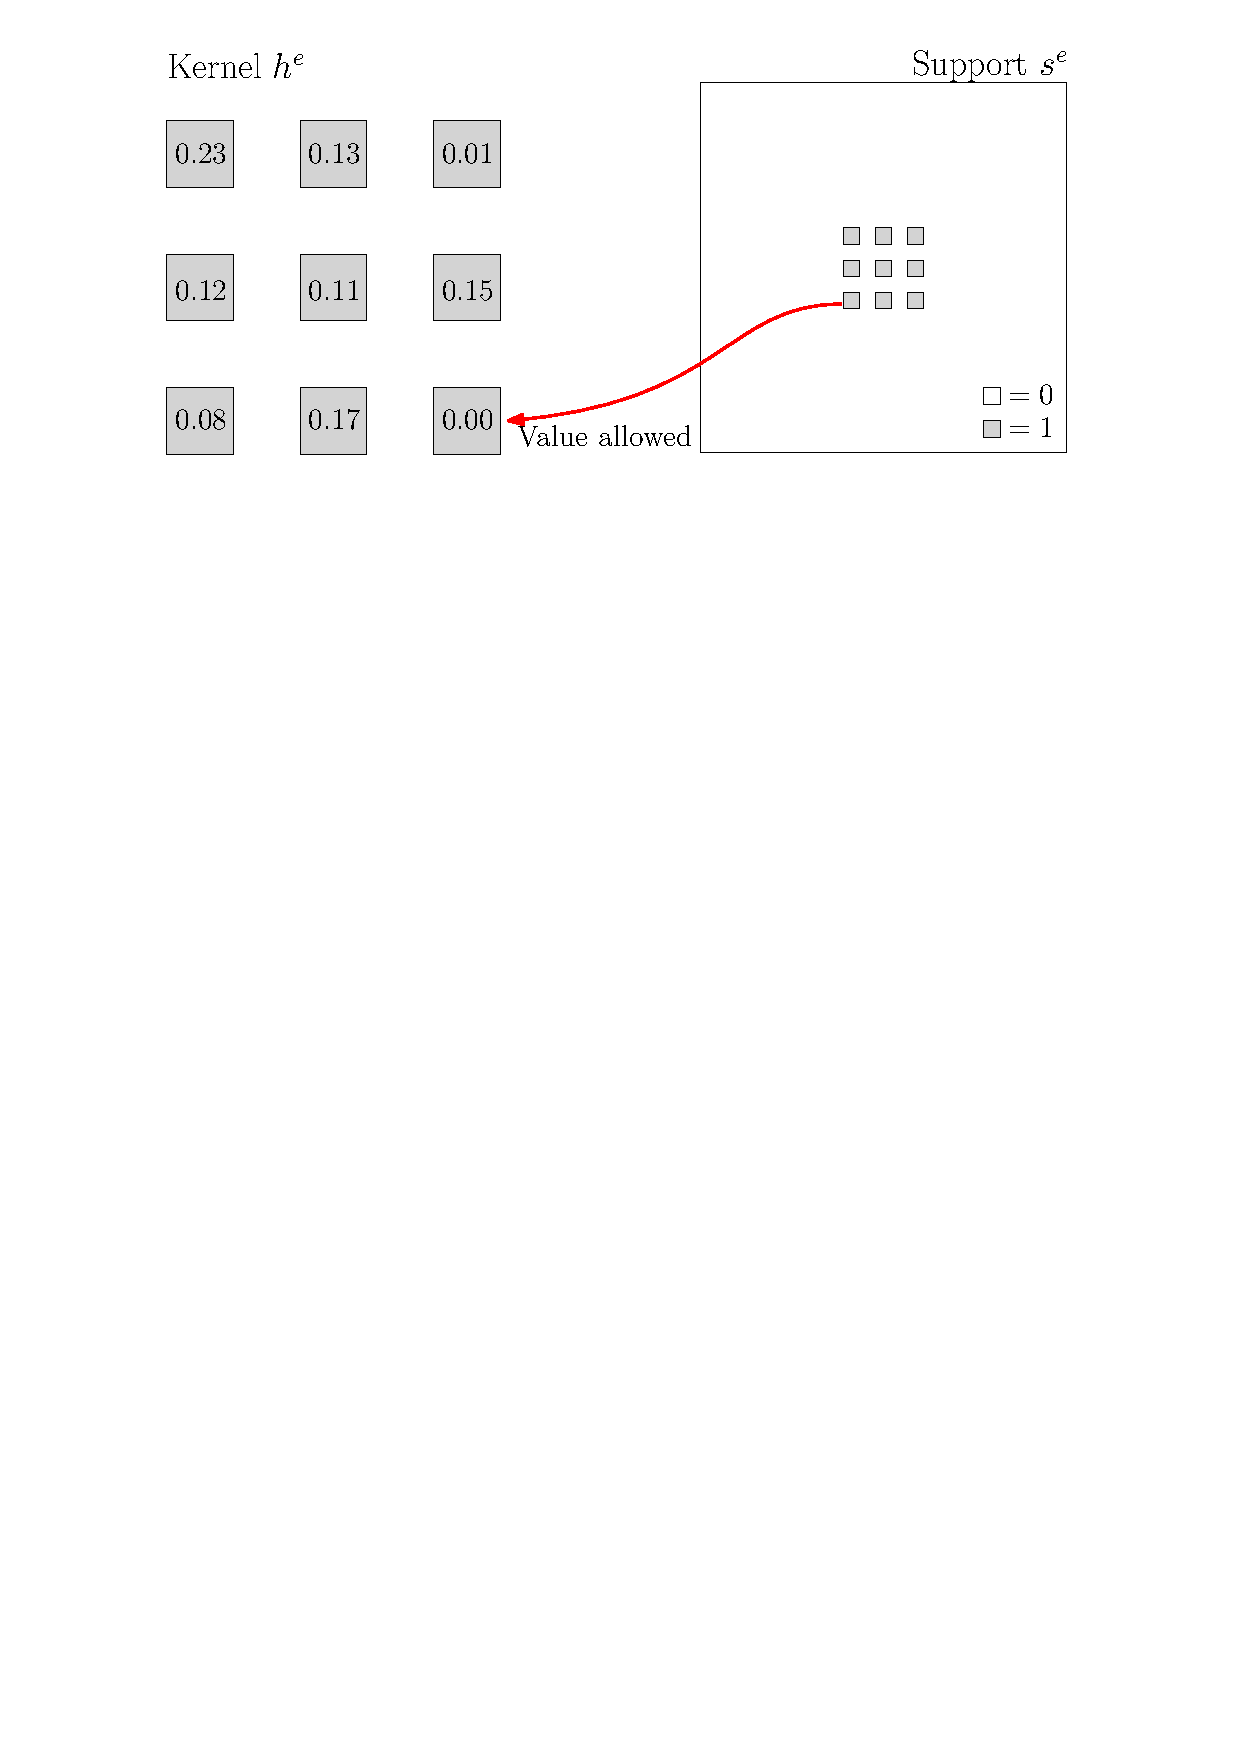
\includegraphics[width=0.80\textwidth]{figures/kernel-h_e.pdf}
\caption{Kernel $\h^e$ (left) and its associated support $\s^e$ (right).}\label{fig_example_kernel}
\end{subfigure}
\end{figure}

One atom of the dictionary $\D$ corresponds to the convolution of successive kernels on a given branch identified by the leaf $l$. We will denote that successive convolution by
$$\h^{*l} = \h^r * \dots * \h^l$$

Using the matrix notation\footnote{See \cref{sec_matrix_vs_tree}}, the convolutional tree dictionary $\D$ applied to a code $\x$ approximates $\y$ as follows
$$\D\x \approx \y$$

The dictionary $\D$ can be written as a matrix (showed in \cref{sec_matrix_vs_tree}). This allows us to compare the computational complexity\todo{REPHRASE} of this dictionary against a simple matrix-vector product. The convolutional tree dictionary computes $\D\x$ using the following formula

\begin{align}
	\D\x = \sum_{l \in \L} \x^l * \h^{*l} \label{eq_Dx_as_convolution}
\end{align}

\subsection{The \acs{FTL} problem}

The dictionary update step associated with the \gls{treemodel} is defined as
\begin{align}
\underset{\substack{(\h^e)_{e}}}\min ~ & \lVert \D\x - \y \rVert_2^2 \tag{$FTL$} \label{eq_ftl}\\
\text{s.t.~} & \s^e_p=0 \Rightarrow \h^e_p = 0 \quad & \forall p=1,\dots,N ,~\forall e \in \E \label{eq_ftl_in_support} \\
 & \lVert \h^e \rVert \le \gamma & \forall e \in \E\label{eq_ftl_kernel_finite_nrj}
\end{align} The constraint in (\ref{eq_ftl_in_support}) guarantees that each kernel $\h^e$ has its non-zero values on the points of its support $\s^e$. Constraint (\ref{eq_ftl_kernel_finite_nrj}) ensures that the overall energy of every support is finite and prevents a specific kernel to “explode”.

\ac{FTL} can be rewritten as an unconstrained problem by introducing a characteristic function $\chi_{\Dspace^e}$ defined for each edge $e$ as follows

\begin{align*}
	\chi_{\Dspace^e}(\h^e) = \begin{cases} 0 &\text{ if } \h^e \in \Dspace^e \\ +\infty & \ \text{otherwise}\end{cases} & \quad \text{with} \quad \Dspace^e = \begin{Bmatrix} \s^e_p=0 \Rightarrow \h^e_p = 0 \quad \forall p=1,\dots,N\\ \text{and }\lVert \h^e \rVert \le \gamma \end{Bmatrix}
\end{align*}

The unconstrained problem is
\begin{align}
\underset{\substack{(\h^e)_{e}}}\min ~ & \lVert \D\x - \y \rVert_2^2 + \sum_{e}\chi_{D_e} (\h^e) \tag{${FTL}_2$} \label{eq_ftl2}
\end{align}

For later references, the objective function of \ac{FTL} will be denoted as
\begin{align}
\Phi[(\h^e)_{e \in \E}] = \lVert \D\x-\y \rVert^2_2
\end{align}

\subsubsection{Interesting properties of \ac{FTL}}

The convolution of sparse kernels in \ac{FTL} leads to theoretically highly performant dictionaries. The computational cost of $\D\x$ using \cref{eq_Dx_as_convolution} is reduced to $O(|\E| S N)$ ($|\E|$ is the number of edges and $S$ the number of elements in all supports). And because $|\E|$ and $S$ are designed to be significantly smaller than $K$ and $N$, using the \gls{treemodel} decreases greatly the cost of using the dictionary and is comparable to the Fourier transform performance (in $O(N \log N)$).

\begin{table}[!ht] \centering 
\caption{Computational cost of $\D\x$} \label{table_comparison_Dx_costs}
\begin{tabular}{c|c}
Using matrix-vector product & Using \gls{treemodel} \\\\ \hline \\
$O(KN)$ & $O(|\E|N)$
\end{tabular}
\end{table}


However, the product $\D\x$ can be seen as a multivariable polynomial of degree the depth of $\T$ (variables are $(\h^e)_{e \in \E}$ and $\x$). This non-linearity makes the objective function possibly strongly non-convex, suggesting that we would end up trapped by its many suboptimal critical points of \ac{FTL}.

And yet, the authors of \cite{chabiron_optimization_2016} have successfully proved that this problem is actually tractable. More surprisingly, they discovered that optimizing \ac{FTL} is possible and that the solutions given by \acs{PALMTREE} are encouraging.


\subsection{The PALMTREE algorithm}\label{sec_palmtree}

The authors of \cite{chabiron_optimization_2016} have shown that \eqref{eq_ftl2} can be solved using the \ac{PALM} algorithm proposed in \cite{bolte_proximal_2014}. The \ac{PALM} algorithm does a proximal gradient iteration successively on the different blocks of variables; \cite{bolte_proximal_2014} provides a proof of convergence towards a critical point for non-convex problems. In our case, one block corresponds to one kernel $\h^e$.


regularizes the non-convex objective function using a simple linear approximation with respect to one block of variables. One block corresponds to one kernel $\h^e$.

The implementation of the generic \ac{PALM} algorithm for solving the \eqref{eq_ftl2} problem has been named \ac{PALMTREE}. 

An outline of the algorithm is given in \cref{alg_palmtree}, where $t^e$ denotes the step size and $\text{prox}^f_\gamma$ is the proximal operator for prior function $f$ defined by $$\text{prox}^f_\gamma(y) = \underset{x}{\argmin}~ f(x) + \frac{\gamma}{2} \lVert x - y \rVert^2_2$$ which, for $f = \chi_{\Dspace^e}$, is easily computed by a projection onto the $\Dspace^e$.

Details on the step size $t^e$ (which requires the computation of a Lipschitz constant) and the proximal operator $\text{prox}^{\chi_{\Dspace^e}}_{t^e}$ are given in \cite{chabiron_optimization_2016}. We will focus on the way the gradient is computed to get more insight from \ac{PALMTREE}.

We define $\H^e$ as the convolution of every branches that crosses the edge $e$ except for the kernel $\h^e$, i.e. $$\H^e = \h^r * \dots * \h^{\text{above}(e)} * \bcancel{\h^{e}} * \sum_{l \in \text{leaves(e)}} \h^{\text{below}(e)^l} * \dots * \h^{l}$$ where $\text{leaves}(e)$ denotes the leaves that can be reached through $e$, $\text{above}(e)$  the edge right above $e$ and $\text{below}(e)^l$ the edge below $e$ that leads to the leaf $l$.

Using this notation, the authors of \cite{chabiron_optimization_2016} have shown that the partial gradient of $\Phi$ w.r.t. $\h^e$ is 
$$\nabla_{\h^e} \Phi[(\h^f)_{f \in \E}] = 2 \H^e * \Res$$ with $\Res$ the residual denoted by
$$\Res = \D\x - \y$$

Because of the projection onto the $\Dspace^e$ unit ball, it is sufficient to compute the partial gradient at the support locations. As explained further in \cref{sec_full_grad}, this means that the convolution $2 \H^e * \Res$ can be efficiently computed using a simple convolution. However, computing the “full” gradient (meaning on every point of kernel $\h^e$) cannot be computed efficiently this way.

\begin{algorithm}[!ht]
    \caption{\ac{PALMTREE} (Proximal Alternating Linearized Minimization for \Gls{treemodel}) algorithm for Dictionary Update}\label{alg_palmtree}
  \begin{algorithmic}[1]
    \Input
    \begin{itemize}
    	\item[--] image $\y$
    	\item[--] tree $\T(\V,\E)$
    	\item[--] codes $(\x^l)_{l \in \L}$
    	\item[--] supports $(\s^e)_{e \in \E}$
    \end{itemize}
    \Output kernels $(\h^e)_{e \in \E} \in \R^{|\E| \times N}$
    \State Initialize $(\h^e)_{e \in \E}$
    \While{not converged}
      \For{$e \in \E$ (depth-first way)}
      	\State $\h^e = \text{prox}^{\chi_{\Dspace^e}}_{t^e} \left(\h^e-\frac{1}{t^e} \nabla_{\h^e} \Phi[(\h^f)_{f \in \E}] \right)$
      \EndFor
    \EndWhile
  \end{algorithmic}
\end{algorithm}



\subsection{Drawbacks}
As explained in \cite[p. 23]{chabiron_optimization_2016}, the main drawbacks to use this \gls{treemodel} for practical dictionary learning (i.e. denoising or image recognition) is that it requires the user to pre-define and fix certain central elements of the model, which is likely to lead to suboptimal results. Among them are the design of the tree (number of children per node, depth) and the choice of the supports.
% NOTE: dictionary learning is an application of machine learning specifically designed for image processing 
\subsubsection{Choice of the tree}
The authors of \cite{chabiron_optimization_2016} used a fixed tree structure, meaning that the tree has been created \emph{ad-hoc} on a per-experiment basis, trying to mimic the frequency pyramid tiling of a curvelet decomposition. The number of leaves was also specifically chosen to match the number of atoms that was generated on the target image.

But getting an actual adaptative dictionary update step implies that the design of the tree is also learned from the example images and incorporated into the formulation of the optimization problem. This research axis has not been explored in this work and will be part of future studies.

\subsubsection{Choice of the supports}

As described in \cref{sec_tree_model}, the supports $\s^e$ are part of the \gls{treemodel}. In \cite{chabiron_toward_2015}, the authors experimentally showed that using fixed supports for approximating many kinds of atoms (curvelets, cosines) is possible. For the specific purpose of approximating existing atoms, the results turned out to be very promising. However, the proposed model was supposed to be able to approximate any kind of image.

So far, the supports have been handcrafted. \Cref{fig_example_kernel} gives an example of typical support layout chosen for the experiments in \cite{chabiron_optimization_2016}. We propose in this work to make the supports “adaptative”, i.e. learning them during the optimization process.

\subsubsection{Still a prototype}
Any actual image processing application would require to learn the dictionary on a large set of images (namely the $\Y$ matrix). However, \ac{PALMTREE} is still unable to handle more than one image.

Moreover, most experiments on \ac{PALMTREE} have been focused on the dictionary update step; real applications would need to alternate between the dictionary update step and the sparse coding step.

\section{Learning the supports}
\todo{Here, explain what my contribution will be...}

\Cref{fig_fixed_vs_expected} illustrates what could be expected to be found as the solution for an “adaptive” support of same size: the support (b) would shape itself into (c) to better match the target atom.

\begin{figure}[!ht]\centering
\begin{subfigure}[b]{0.32\textwidth}\centering
	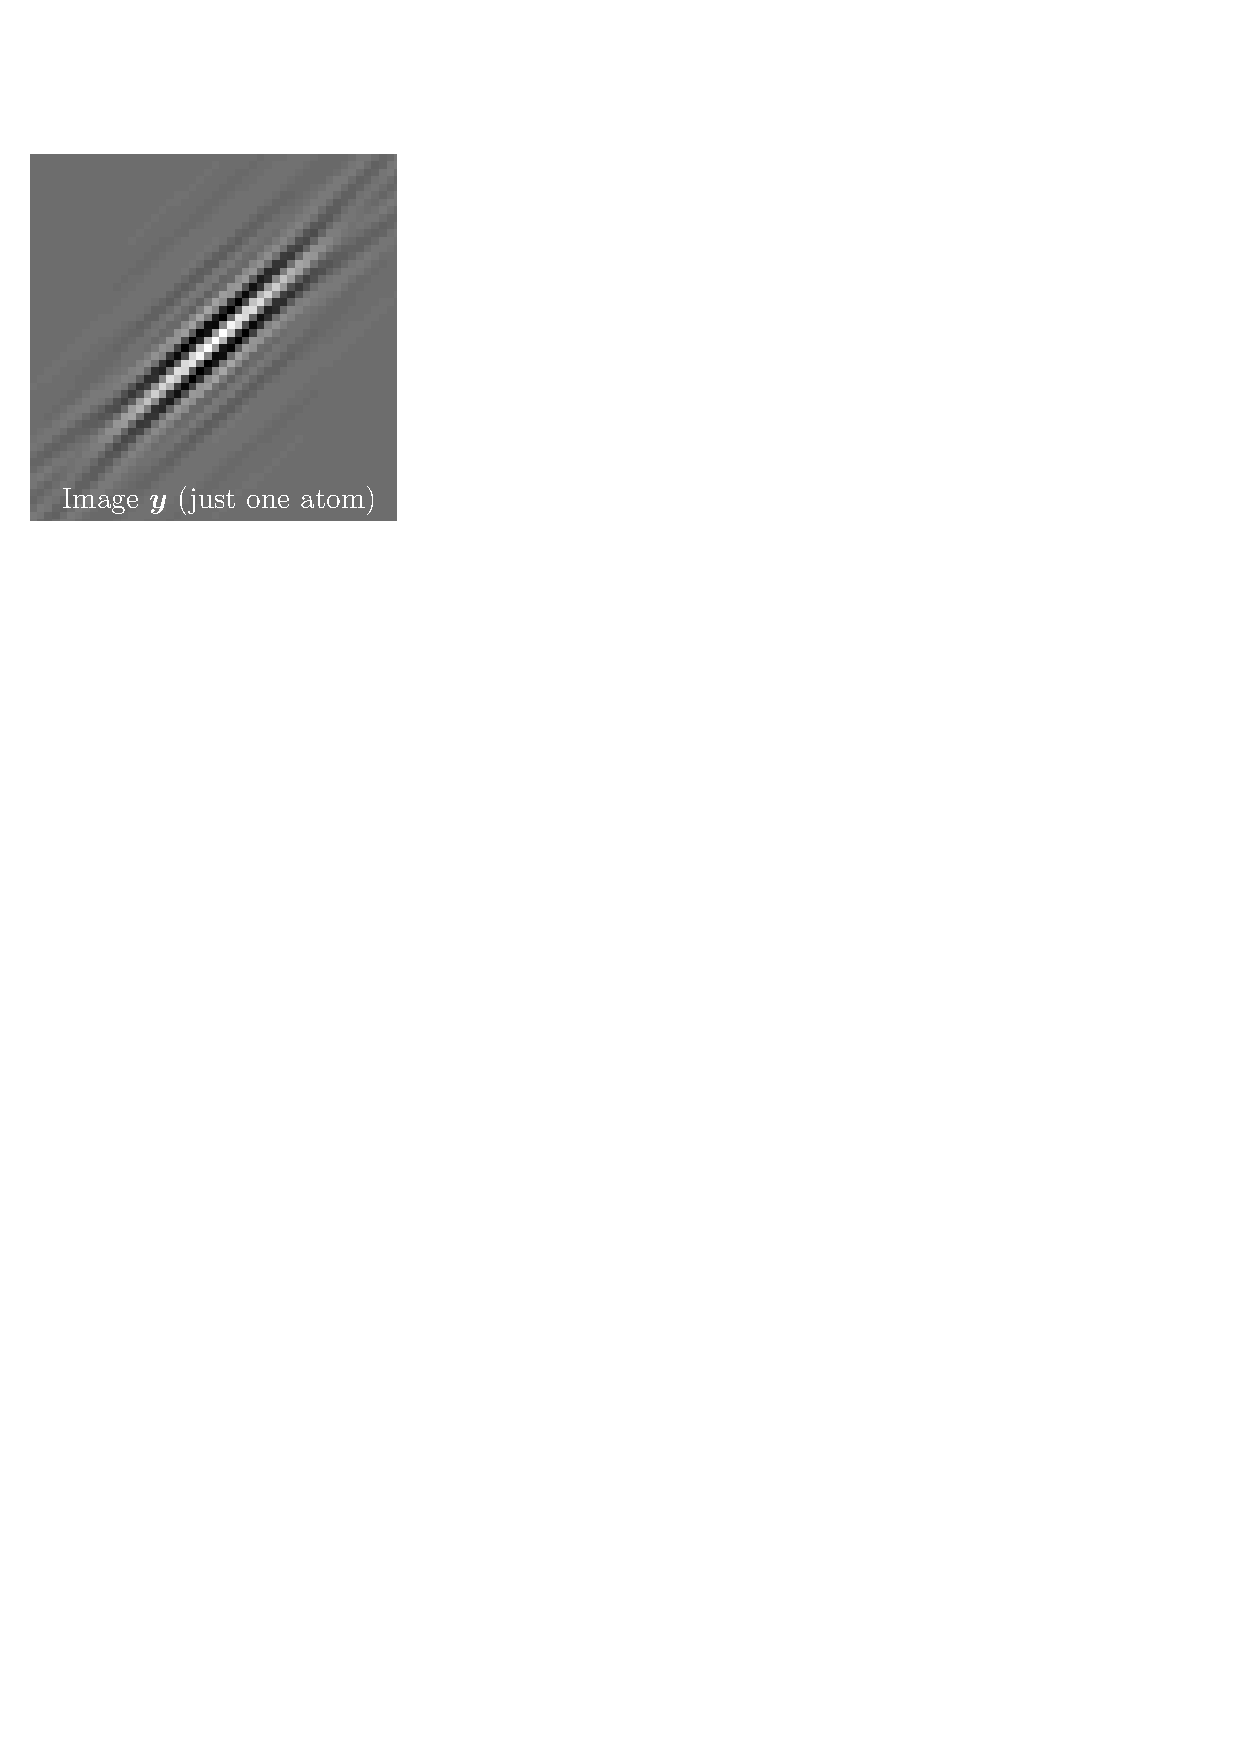
\includegraphics[width=\textwidth]{figures/manual-better-support/target.pdf}
	\caption{}\label{fig_fixed_vs_expected_y}
\end{subfigure}
\begin{subfigure}[b]{0.32\textwidth}\centering
	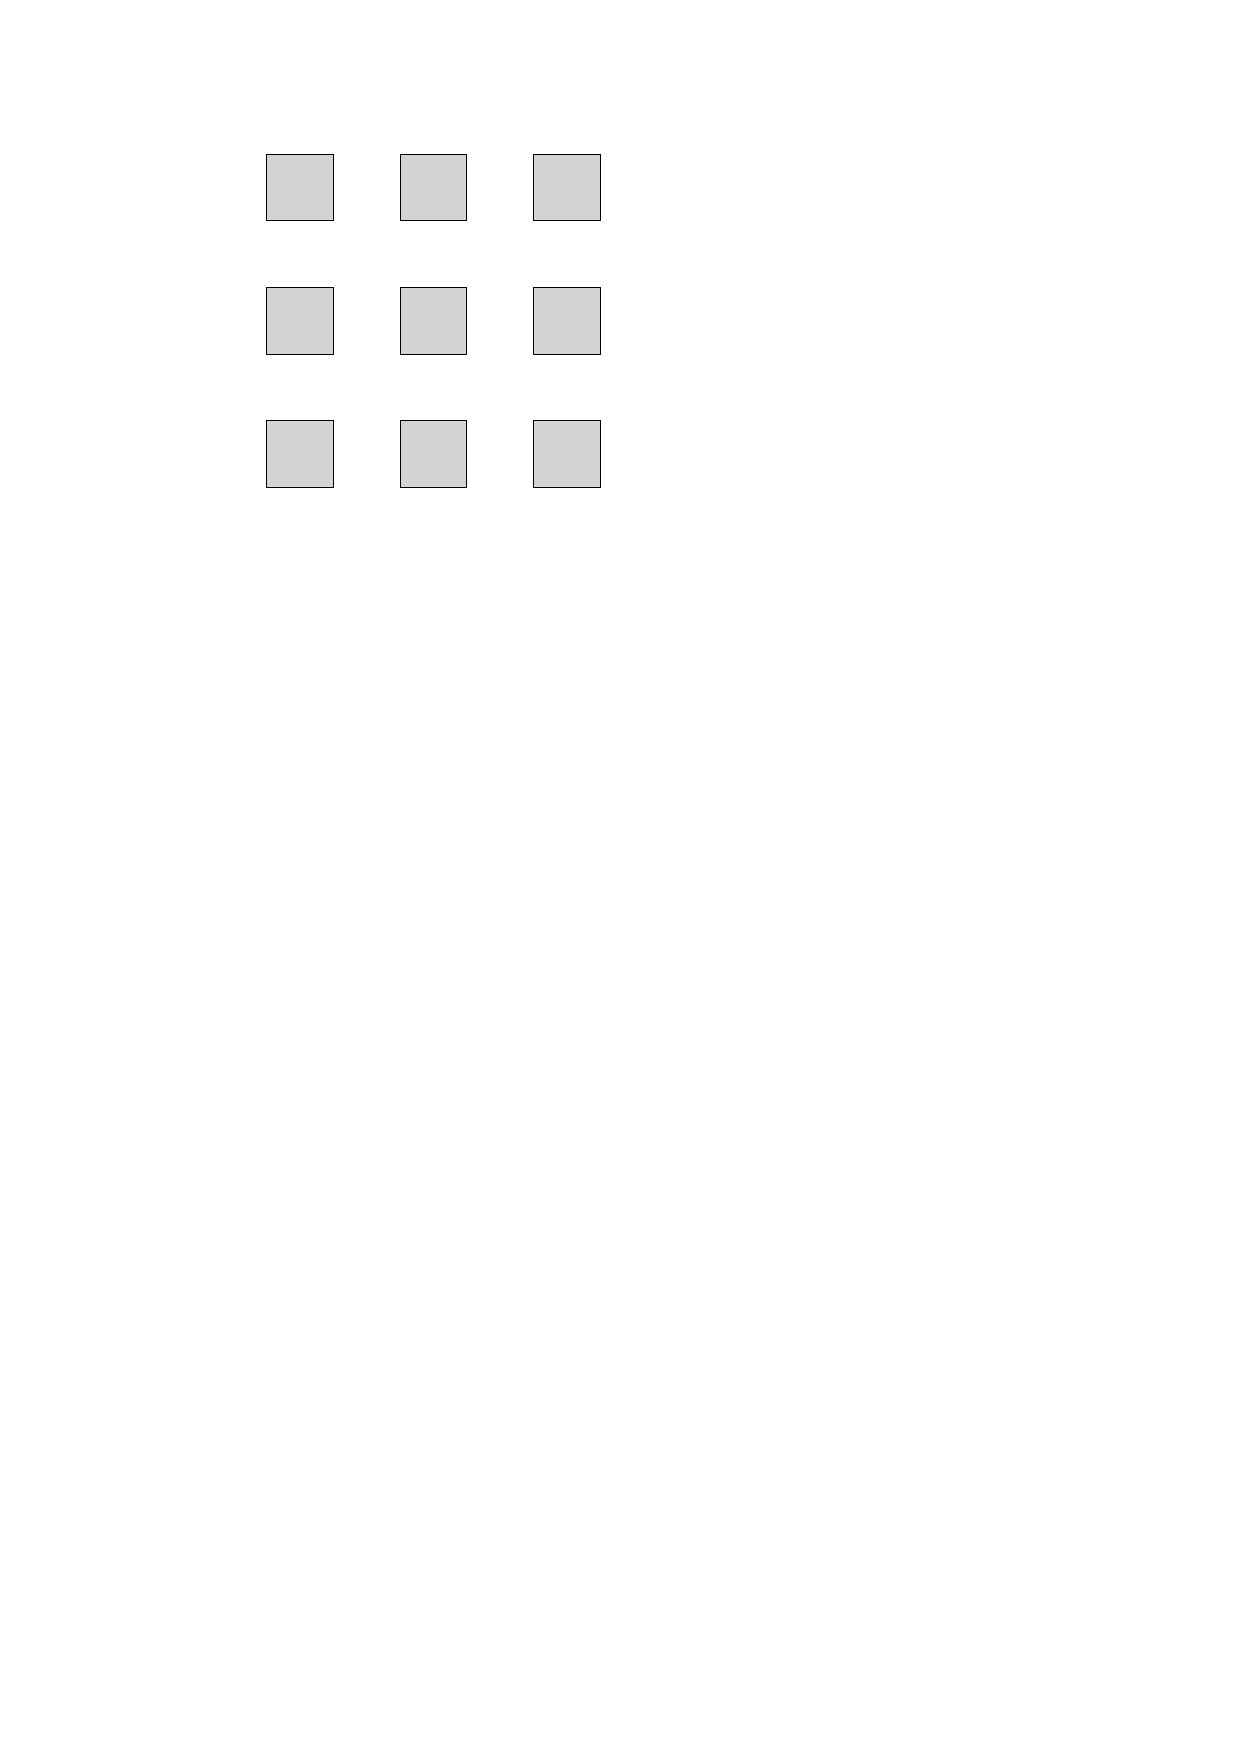
\includegraphics[width=0.5\textwidth]{figures/manual-better-support/support.pdf}
	\caption{Generic support}
\end{subfigure}
\begin{subfigure}[b]{0.32\textwidth}\centering
	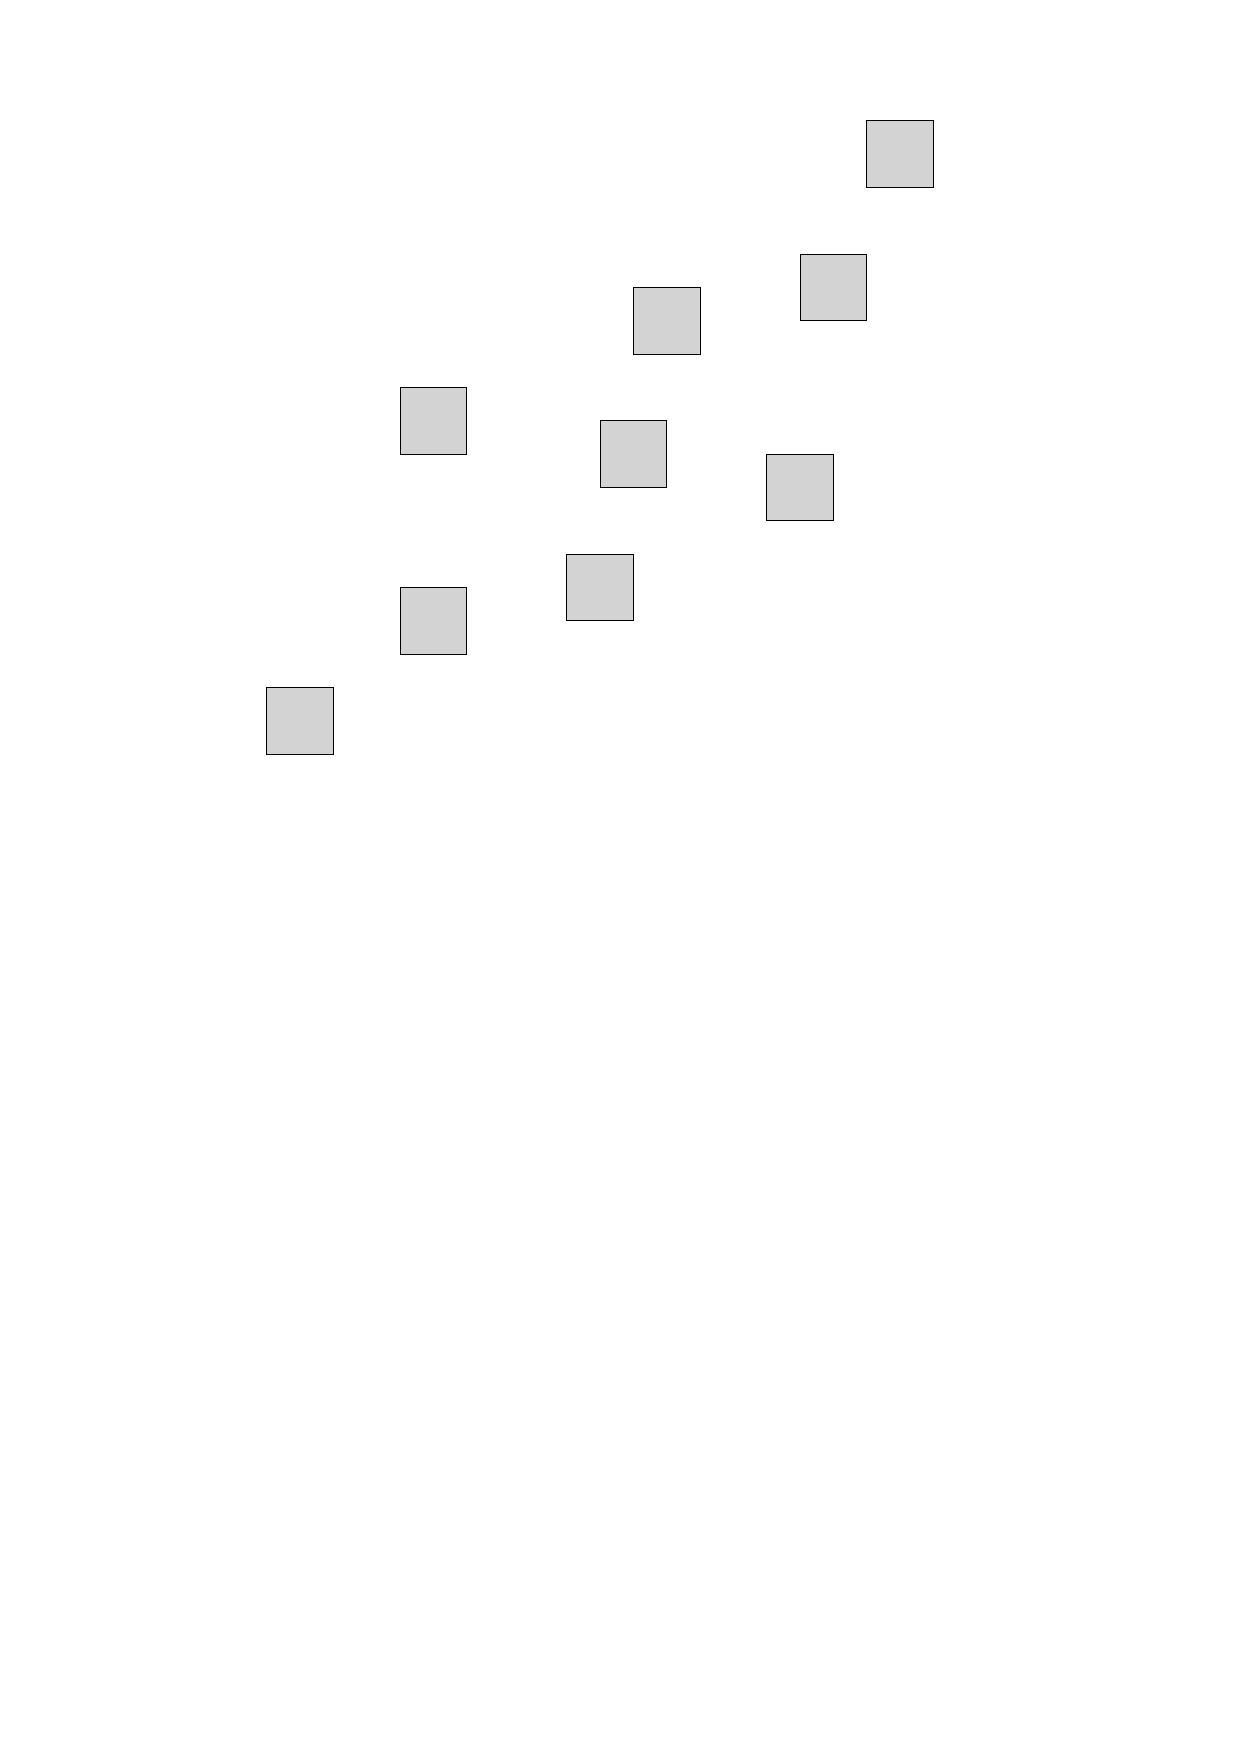
\includegraphics[width=\textwidth]{figures/manual-better-support/support-better.pdf}
	\caption{Expected support}
\end{subfigure}
\caption{Generic versus expected supports. (a) is the target image made of one curvelet. (b) gives the locations of the support elements for one edge of the tree. (c) shows a handcrafted support that we expect to be giving better results as it follows the general direction of the curvelet}\label{fig_fixed_vs_expected}
\end{figure}

\Cref{fig_xp_fixed_vs_expected} experimentally confirms the assumption made in \Cref{fig_fixed_vs_expected}. We switched $\s^4$ from a generic (\textit{a priori}) support to a hand-made support that follows the general direction of $\y$ (\cref{fig_fixed_vs_expected_y}). The RMSE\footnotemark[1] is decreased by -16\% (lower is better). The approximation in \cref{fig_xp_fixed_vs_expected_approx2} looks visually better than the one in \cref{fig_xp_fixed_vs_expected_approx1}.

\footnotetext[1]{Root mean square error. Let $\y^1$ and $\y^2$ two images of concatenated into a vector of dimension $N$, then $RMSE(\y^1,\y^2) = \frac{1}{N} \sqrt{\sum_{i=1}^N (y^1_i - y^2_i)^2}$}

\begin{figure}[!ht]\centering
\begin{subfigure}[b]{0.085\textwidth}\centering
	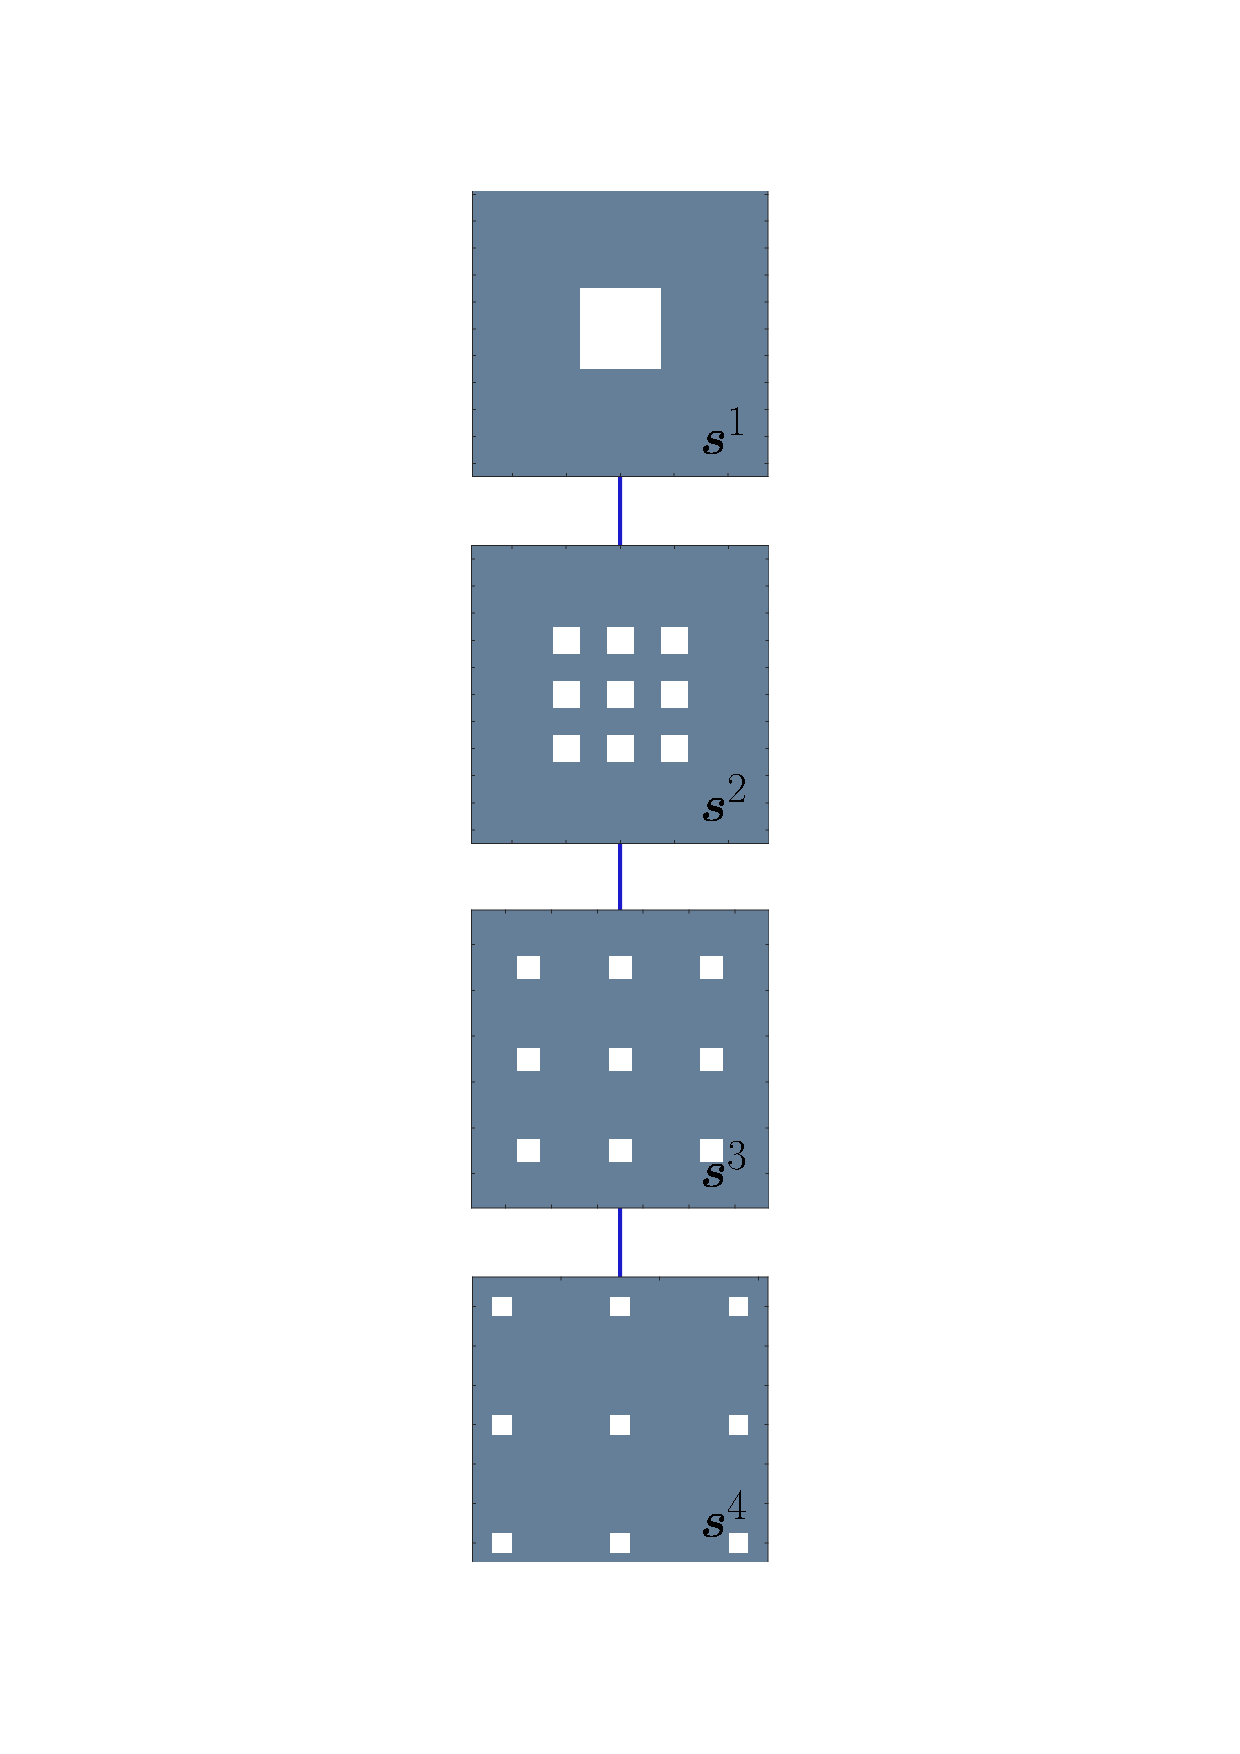
\includegraphics[width=\textwidth]{figures/exple-better-support/tree_classic.pdf}
	\caption{}
\end{subfigure}
\begin{subfigure}[b]{0.39\textwidth}\centering
	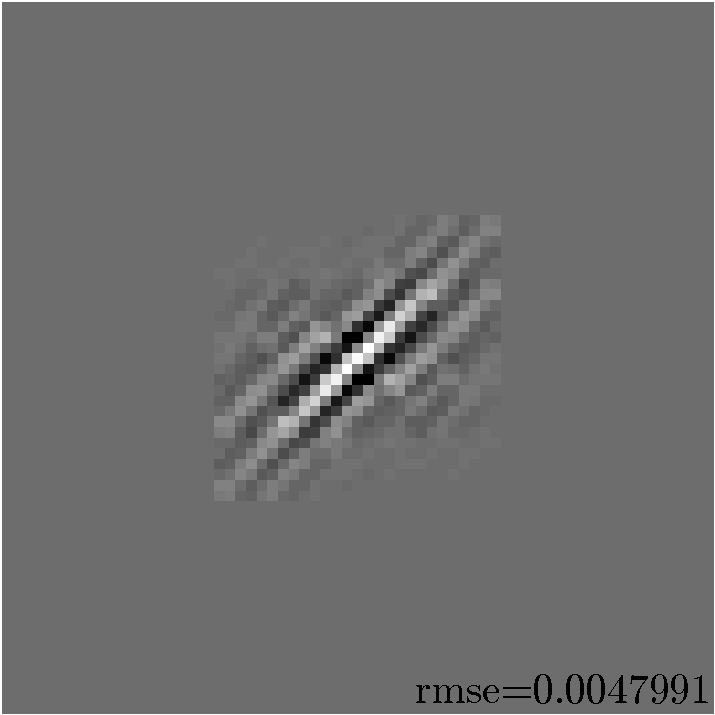
\includegraphics[width=\textwidth]{figures/exple-better-support/xp_128x128_sc2_angl1_K3_S3_node4classic_approx.pdf}
	\caption{$\D\x$ with generic supports}\label{fig_xp_fixed_vs_expected_approx1}
\end{subfigure}
\begin{subfigure}[b]{0.085\textwidth}\centering
	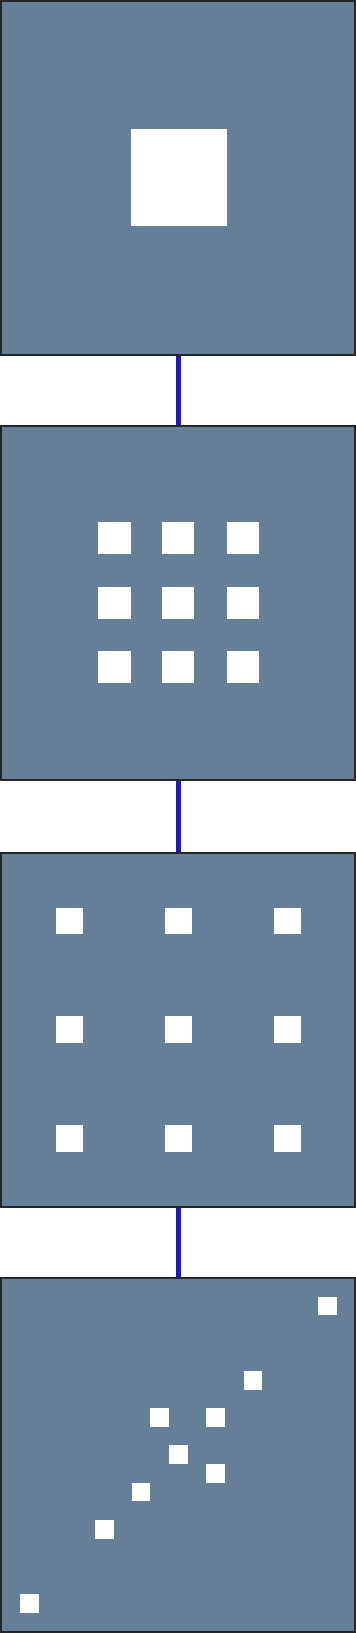
\includegraphics[width=\textwidth]{figures/exple-better-support/tree_expected.pdf}
	\caption{}
\end{subfigure}
\begin{subfigure}[b]{0.39\textwidth}\centering
	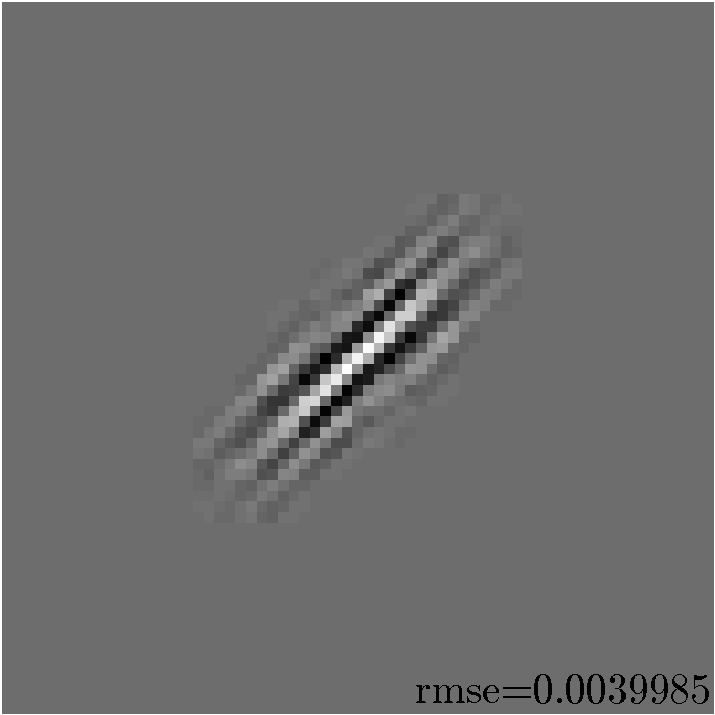
\includegraphics[width=\textwidth]{figures/exple-better-support/xp_128x128_sc2_angl1_K3_S3_node4expected_approx.pdf}
	\caption{$\D\x$ with handcrafted $\s^4$}\label{fig_xp_fixed_vs_expected_approx2}
\end{subfigure}
\caption{Visual enhancement when adapting a support.} \label{fig_xp_fixed_vs_expected}
\end{figure}




\chapter{Experiments}

This chapter covers the protocols and results of the various experiments aimed to learning the supports during the \ac{PALMTREE} algorithm.

\section{Experiment setup}
Every experiment in this chapter is using a fixed single-branch tree of depth 4 associated with $\y$, $\h^e$, $\s^e$ and $\x^e$ of size $128 \times 128$. The figures only display the central $64 \times 64$ pixels as shown in \cref{fig_xp_explain}.

\begin{figure}[!ht]\centering
\begin{subfigure}[b]{0.32\textwidth}\centering
	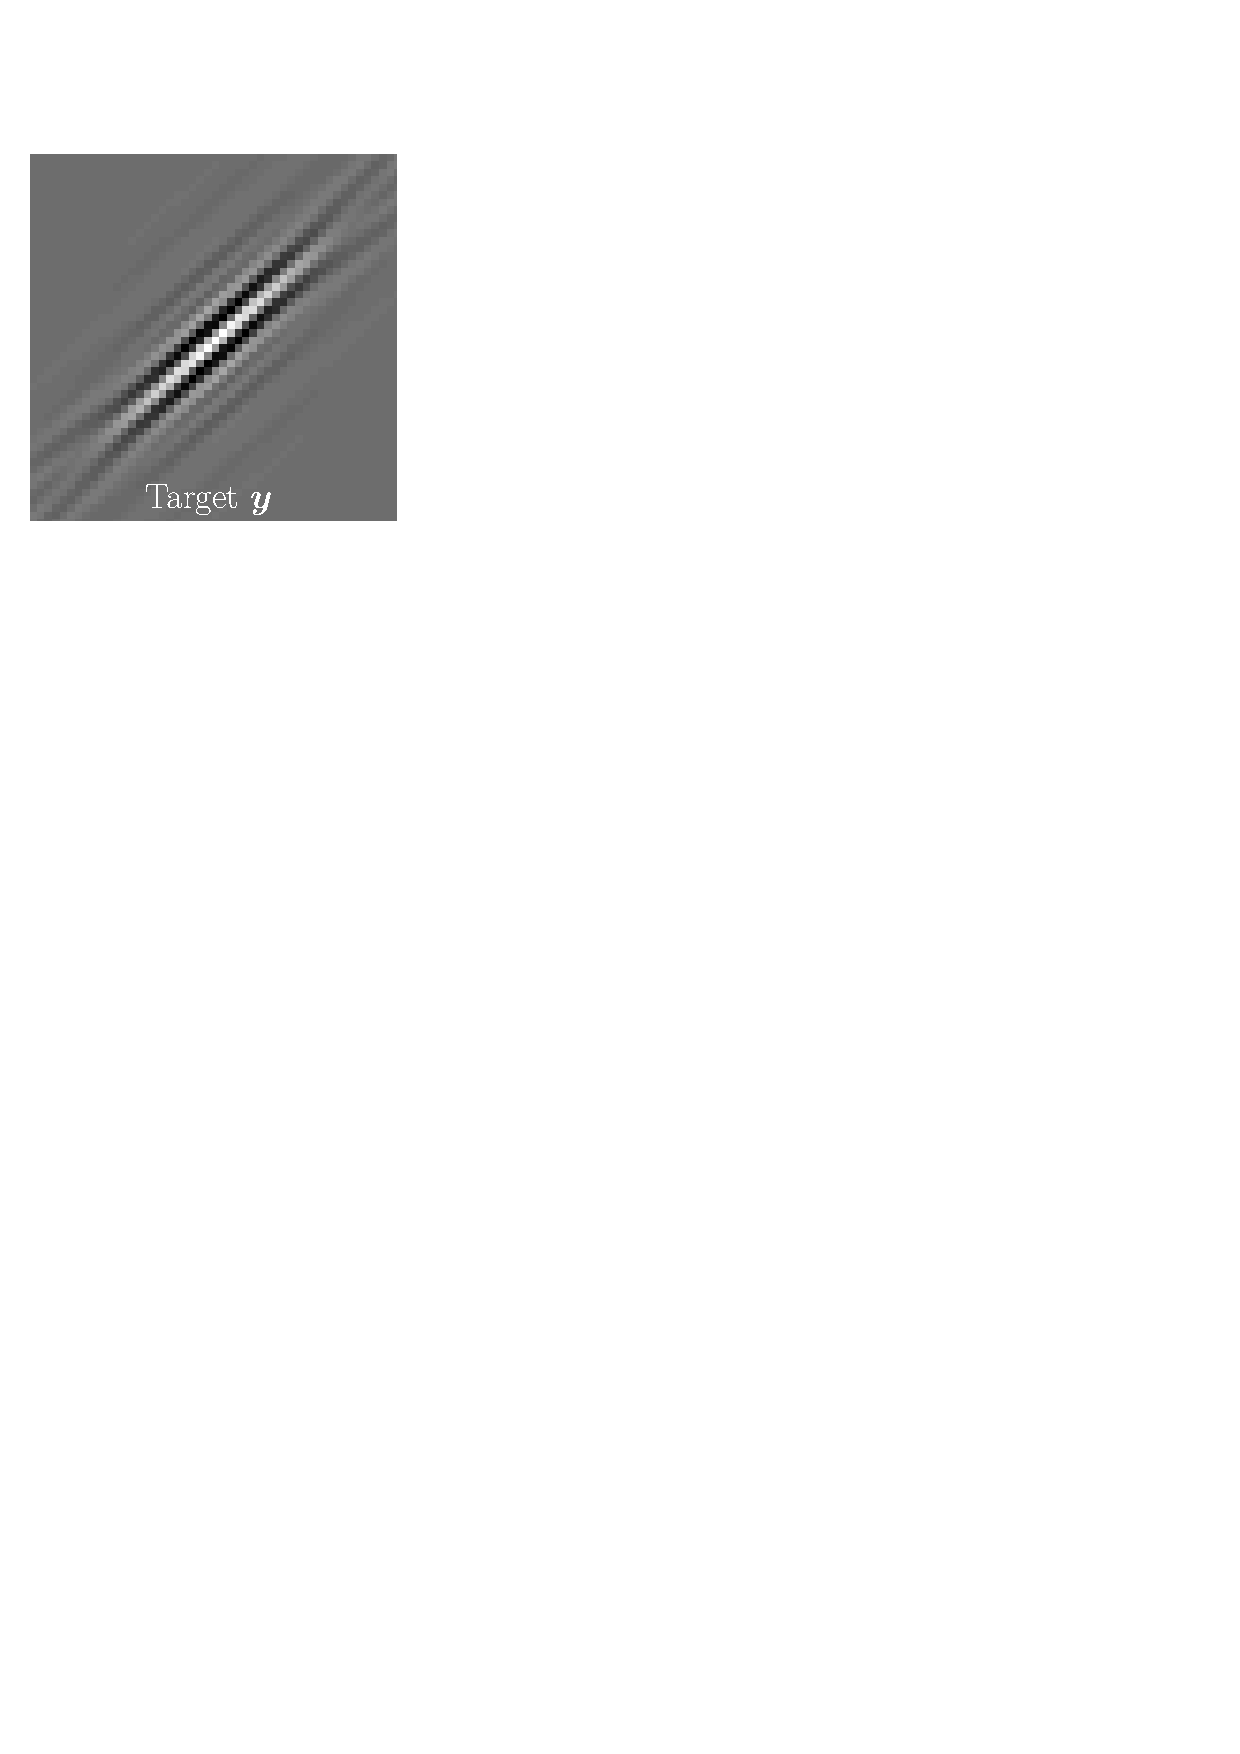
\includegraphics[width=0.9\textwidth]{figures/xp_explain/target.pdf}
	\caption{}
\end{subfigure}
\begin{subfigure}[b]{0.32\textwidth}\centering
	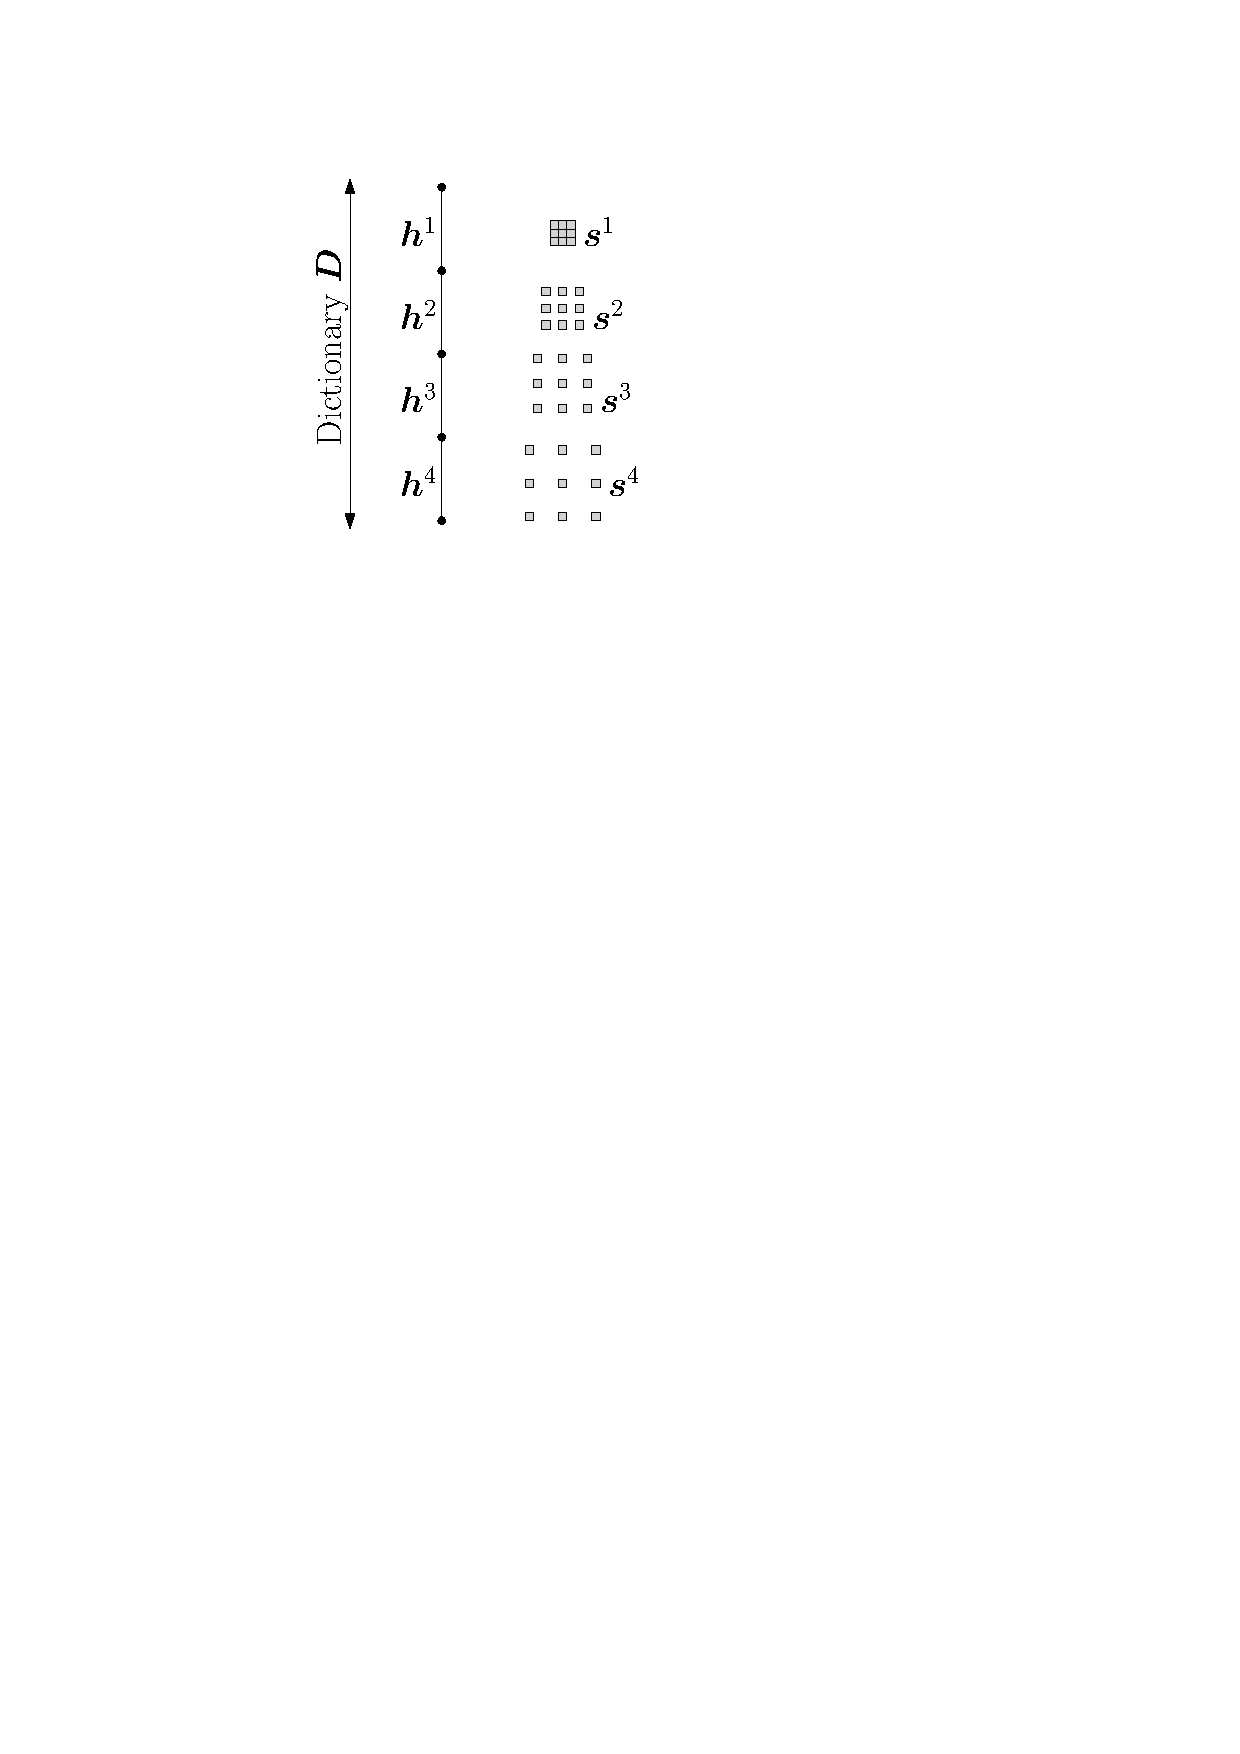
\includegraphics[width=0.9\textwidth]{figures/xp_explain/dictionary.pdf}
	\caption{}
\end{subfigure}
\begin{subfigure}[b]{0.32\textwidth}\centering
	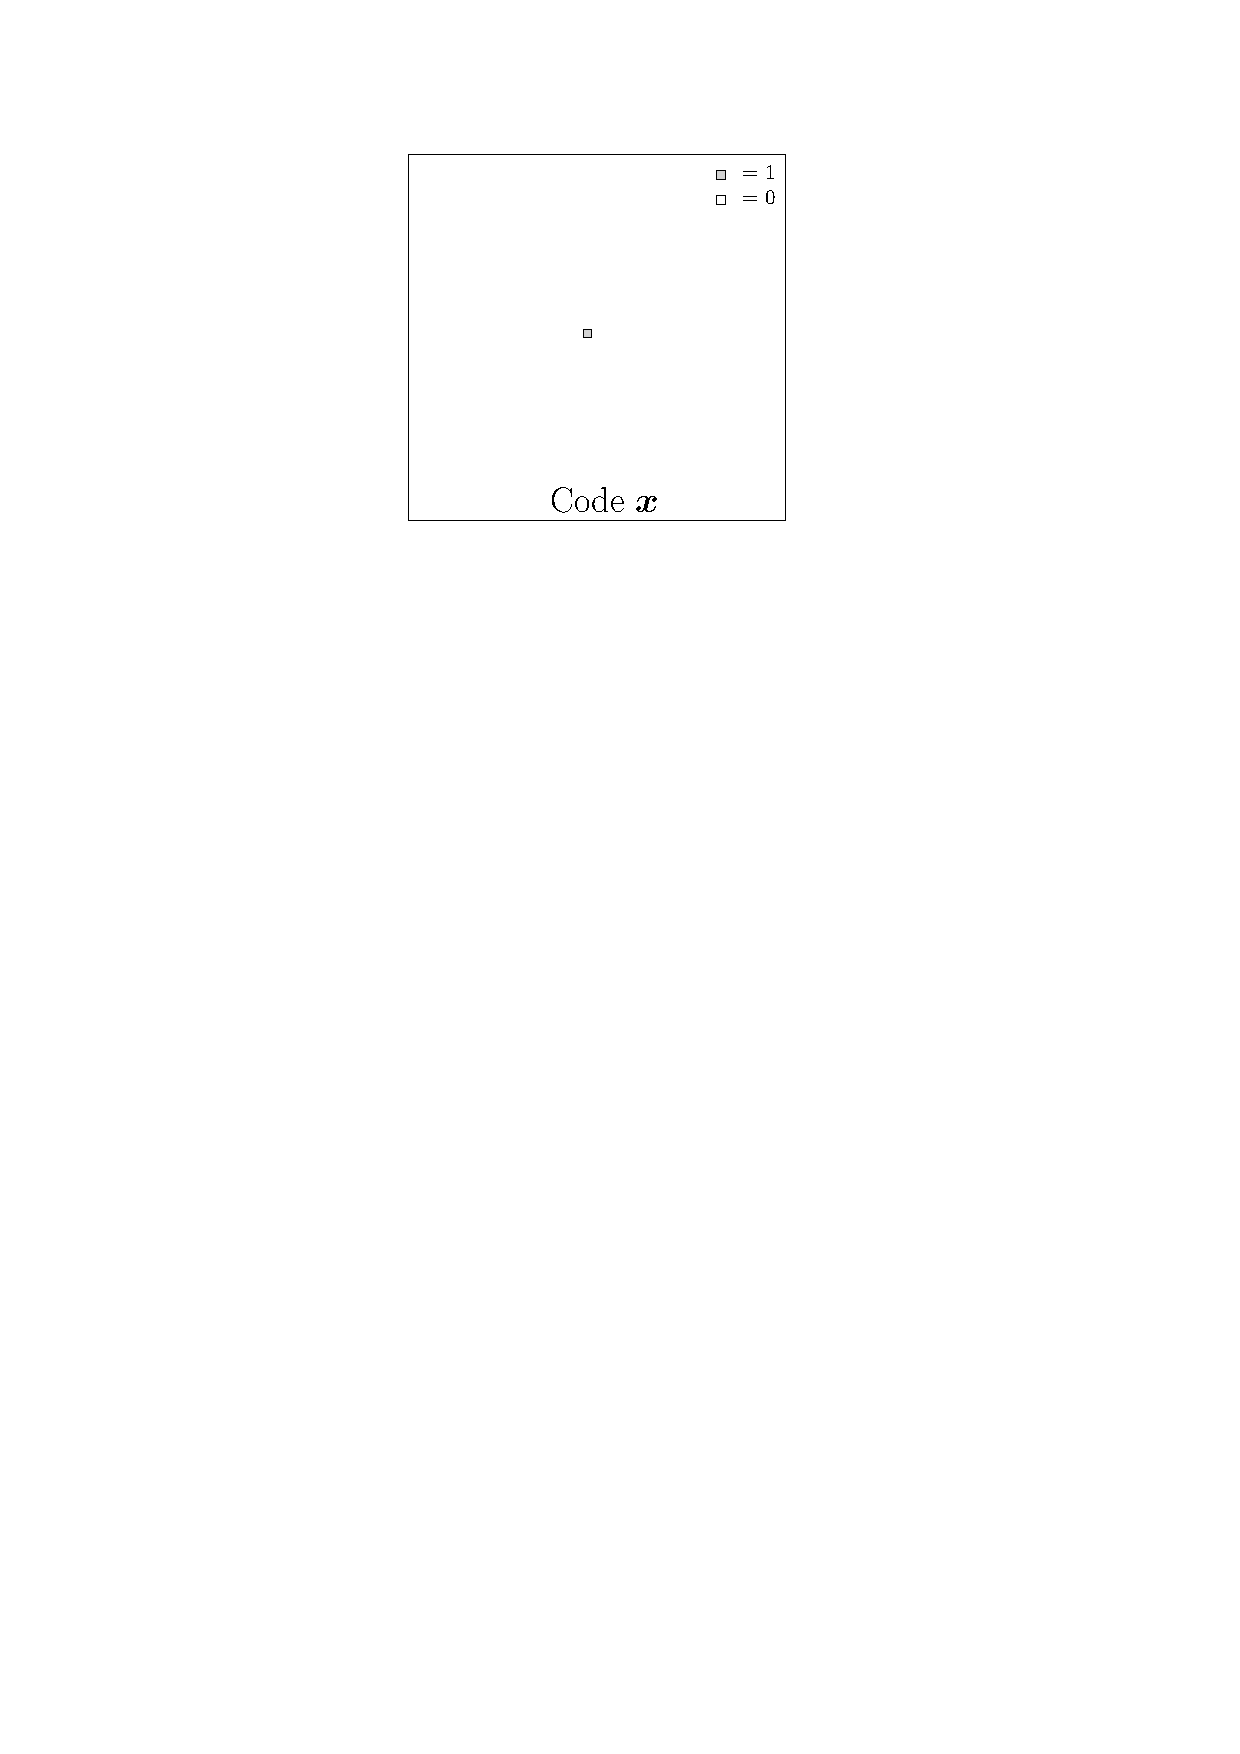
\includegraphics[width=0.9\textwidth]{figures/xp_explain/code.pdf}
	\caption{}
\end{subfigure}
\caption{Experiment setup. The experiments are using one image $\y$, one dictionary $\D$ (formed by $\T$, $(\s^e)_{e \in \E}$, $(\h^e)_{e \in \E}$) and one $\x$. The parameters $\y$, $\x$, $\T$, $(\s^e)_{e \in \E}$ are given and $(\h^e)_{e \in \E}$ is learned (the only variable).}\label{fig_xp_explain}
\end{figure}
The experiment’s dictionary associated to this convolutional tree can be simply written as
$$\D\x = \h^1 * \h^2 * \h^3 * \h^4 * x$$

\section{Using the gradient for choosing the element to add}

The Orthogonal Matching Pursuit (\ac{OMP}, detailed in \cref{alg_omp}) chooses which component $\x_i$ should be “turned on” at each iteration, finding the atom $d_i$ that has the greatest correlation with the residual $\Res$. This step (cf. \cref{alg_omp_pick_correlation}) uses the gradient $\nabla \Phi(\x)$, with $$\Phi(\x) = \lVert \D\x - \y \rVert^2$$


\begin{algorithm}[!ht]
    \caption{Orthogonal Matching Pursuit (OMP) algorithm for sparse approximation}\label{alg_omp}
  \begin{algorithmic}[1]
    \Input signal $\y$ of dimension $N$, dictionary of dim $N \times K$ with $K \gg N$
    \Output A $k$-sparse code $\x$ of dimension $K$
    \State \textbf{Initialization} $S=\{\}$
    \For{$i = 1,\dots,k$}
      \State $j =  \underset{j = 1,\dots,K}{\argmax} | \nabla \Phi(\x)_j |$ \label{alg_omp_pick_correlation}\Comment{find atom with max. correlation with residual $\Res$}
      \State $S = S \cup \{j\}$
      \State $\x = \underset{\text{supp}(\x) \subset S}{\argmin} \Phi(\x)$
    \EndFor
  \end{algorithmic}
\end{algorithm}

Our idea is to use the same principle when adding elements to supports $(\s^e)_{e \in \E}$: add a new element to one of the supports between two minimizations of the \ac{PALMTREE} algorithm, using the greatest gradient component information.

\Cref{alg_omppalmtree} gives an adaptation of the \ac{OMP} algorithm for the \gls{treemodel}.

\begin{algorithm}[!ht]
    \caption{\ac{OMP} algorithm using \ac{PALMTREE}}\label{alg_omppalmtree}
  \begin{algorithmic}[1]
    \Input signal $\y$ of dimension $N$, dictionary of dim $N \times K$ with $K = |\E| \times N$ and $K \gg N$
    \Output A $k$-sparse code $\x$ of dimension $K$
    \State \textbf{Initialization} Initialize the supports $\s^e$ such that $k=1$
    \For{$i = 1,\dots,k$}
      \State $(e,p) = \underset{(e,p) \in \E \times \P}{\argmax}~ |\nabla \Phi_{\h^e}(\h)_p|$\Comment{Choose support $s^e$ and location $p$} \label{alg_omppalmtree_find}
      \State $\s^e_p = 1$
      \State $\h = \underset{\h^e \in \Dspace^e}{\argmin}~ \Phi(\h)$ \Comment{Solve \eqref{eq_ftl} using \ac{PALMTREE}} \label{alg_omppalmtree_ftl}
    \EndFor
  \end{algorithmic}
\end{algorithm}


However, three questions rose when designing this new “meta” algorithm:
\begin{enumerate}[label={\alph*)},noitemsep]
	\item At \cref{alg_omppalmtree_find}, is it actually correct to choose the element to be added using a strictly local information of the gradient?
	\item Also at \cref{alg_omppalmtree_find}, how would we get the “full” gradient while the current gradient is only computed on the points of the support?
	\item Finally, at (\cref{alg_omppalmtree_ftl}), is it really necessary to wait for the convergence of \eqref{eq_ftl}?
\end{enumerate}
  Also, 

We will first review how the “full” gradient is computed and then describe a way to check that the “full” gradient gives a good direction towards a critical point, comparing it with what we call “gain-per-added-point”. Finally, we will give some thoughts on whether we should wait for \eqref{eq_ftl} to converge or if some iterations suffice between two iterations of \cref{alg_omppalmtree}.


\subsection{Computing the “full” gradient} \label{sec_full_grad}
Up to now, the gradient was computed using a convolution based on translations, as mentioned in \cref{sec_palmtree}. It takes advantage of the sparsity of each kernel $\h^e$ as well as the fact that the proximal operator is projecting every kernel onto its support, meaning that only a few elements have to be computed.

We basically chose to use the fast Fourier transform ($\F$) for computing the convolution on the whole kernels:
\begin{align*}
	\nabla_{\h^e} \Phi((\h^f)_{f \in \E})&= \F^{-1}(\F(\H^{e})^* \circ \F(\Res))
\end{align*}
with ${}^*$ denoting the adjoint operator, $\circ$ the Hadamard product (point-wise product); $\H^{e}$ as well as $\Res$ are notations defined in \cref{sec_palmtree}. \todo[]{should I talk about the complexity of such using Fourier instead of the “sparse” convolution we use for the “restrained” gradient?}

\subsection{Validation of the “full” gradient}
We had some trouble when trying to compute the gradient on the full kernels $(\h^e)_{e \in \E}$ (not only on the supports element locations). To be sure that the computed “full” gradient was correct, we compared it to a finite-difference gradient:

$$\lim_{\epsilon \rightarrow 0} \frac{\Phi((\h^e)_{e \in \E}+\epsilon e_i) - \Phi ((\h^e)_{e \in \E}) }{\epsilon} ~=~ \nabla_i \Phi ((\h^e)_{e \in \E})$$

\begin{figure}[!ht]\centering
\begin{subfigure}[b]{0.30\textwidth}\centering
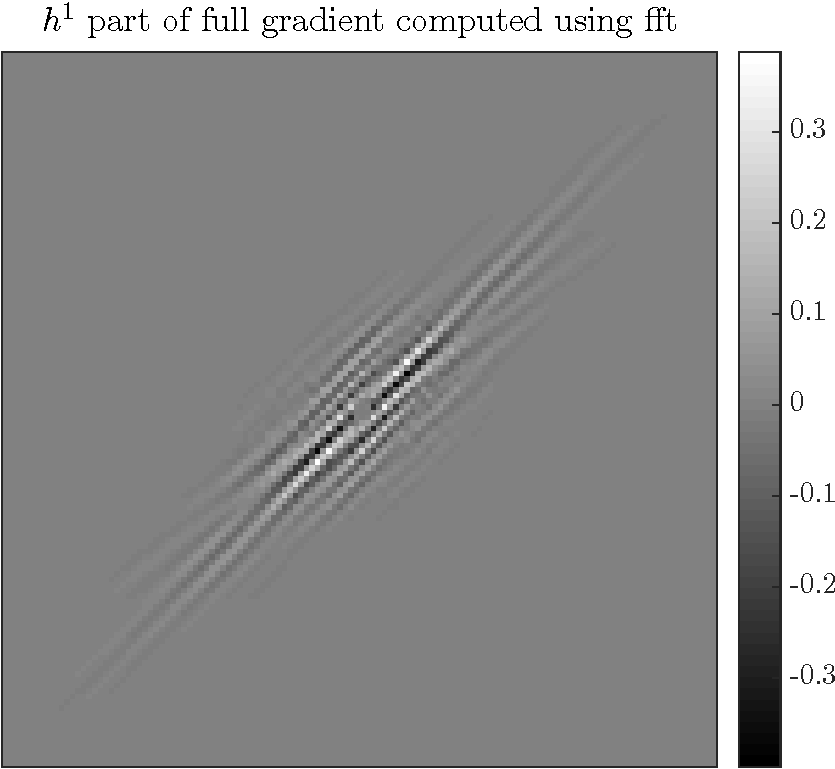
\includegraphics[width=\textwidth]{figures/verif_gradient/gradient.pdf}
\caption{“Full” gradient}
\end{subfigure}
\begin{subfigure}[b]{0.30\textwidth}\centering
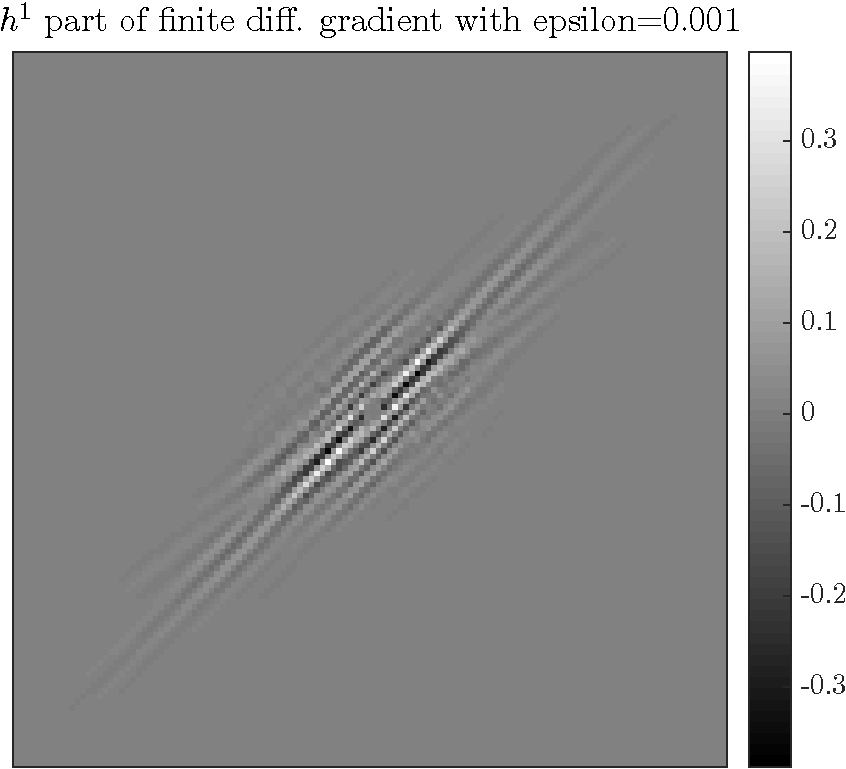
\includegraphics[width=\textwidth]{figures/verif_gradient/finite-diff.pdf}
\caption{Finite-difference}
\end{subfigure}
\begin{subfigure}[b]{0.35\textwidth}\centering
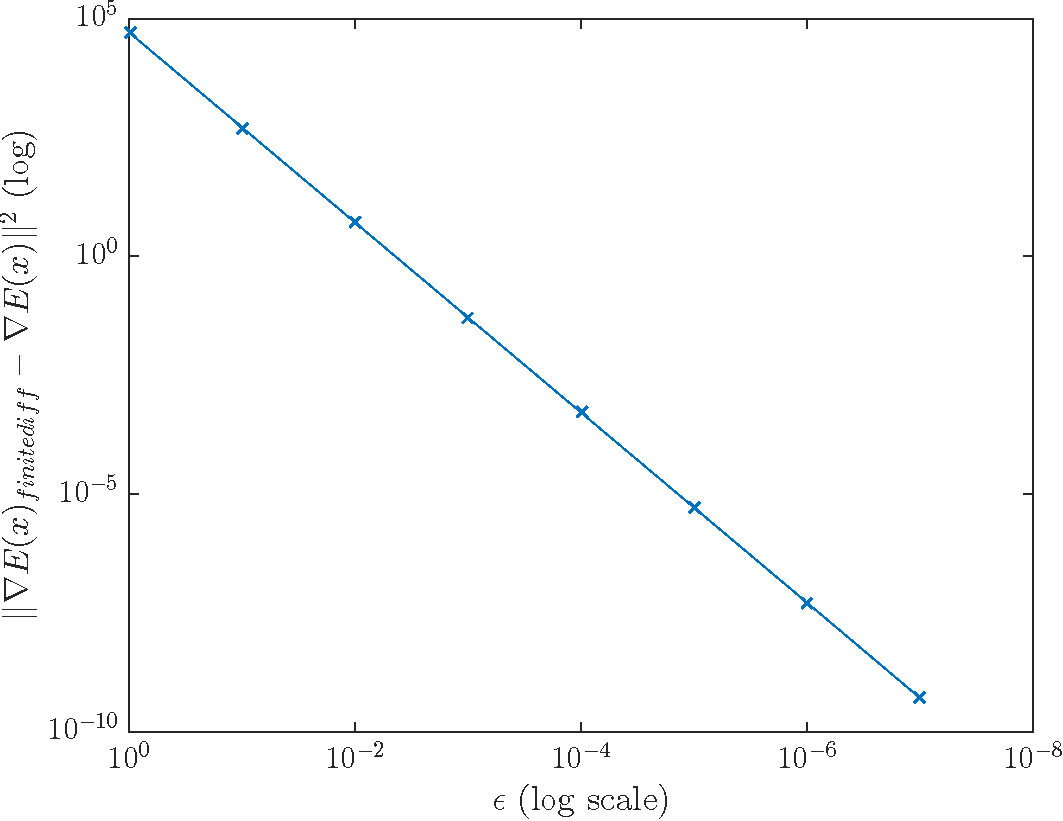
\includegraphics[width=\textwidth]{figures/verif_gradient/finite-diff-vs-grad.pdf}
\caption{Error w.r.t. $\epsilon$}
\end{subfigure}
\caption{Checking that the “full” gradient is correct. We compare it to the finite-difference gradient and make the $\epsilon$ tend to 0.} \label{fig_verif_gradient}
\end{figure}

Figure \ref{fig_verif_gradient} compares the FFT-computed gradient to the finite-difference gradient (with $\epsilon=0.001$). The bottom left figure shows that the two gradients are very close in term of difference. The right figure shows that the finite-difference gradient converges to the “full” gradient, which confirms that our “full” gradient is correct.

\section{Gain-per-added-point to the support}\label{sec_gain_per_added_point}

This section details the method used for making sure that the “full” gradient is appropriate for adding points to supports at \cref{alg_omppalmtree_find} in \cref{alg_omppalmtree}.

\begin{algorithm}[!htb]
    \caption{Gain-per-added-point $\g^f$ for the support $\s^f$}\label{alg_gain_per_added_point}
  \begin{algorithmic}[1]
    \Input One chosen edge $f \in \E$ and a tree $\T$, supports $\s$ and kernels $\h$
    \Output $\g^f$, the gain per added point for support $\s^f$
    \State $\k = \underset{\h}{\argmin}~ \Phi (\h)$ \quad s.t.~$\h^e \in \Dspace^e$ \quad $\forall e \in \E$ \Comment{common starting point}
    \For{each point $p$ of $\s^f$}
    	\State $\s^f_p = 1$ \Comment{add element to support}
    	\State Initialize $\h = \k$
    	\State $\g^f_p = \Phi(\k) - \underset{\h}{\min}~ \Phi (\h)$ \quad s.t.~$\h^e \in \Dspace^e$ \quad $\forall e \in \E$
    	\State $\s^f_p = 0$ \Comment{remove element to support}
    \EndFor
  \end{algorithmic}
\end{algorithm}

We designed \cref{alg_gain_per_added_point} for computing what we call the \emph{gain-per-added-point} matrix, denoted $\g^f$ ($f$ is the edge of the studied support). \Cref{alg_gain_per_added_point} tries every possible point that could be added to one given support $s^f$ and see how much the objective function decreases when adding the point and continuing the minimization.

\begin{figure}[!h]\centering
\begin{subfigure}[b]{0.8\textwidth}\centering
\begin{subfigure}[b]{0.49\textwidth}\centering
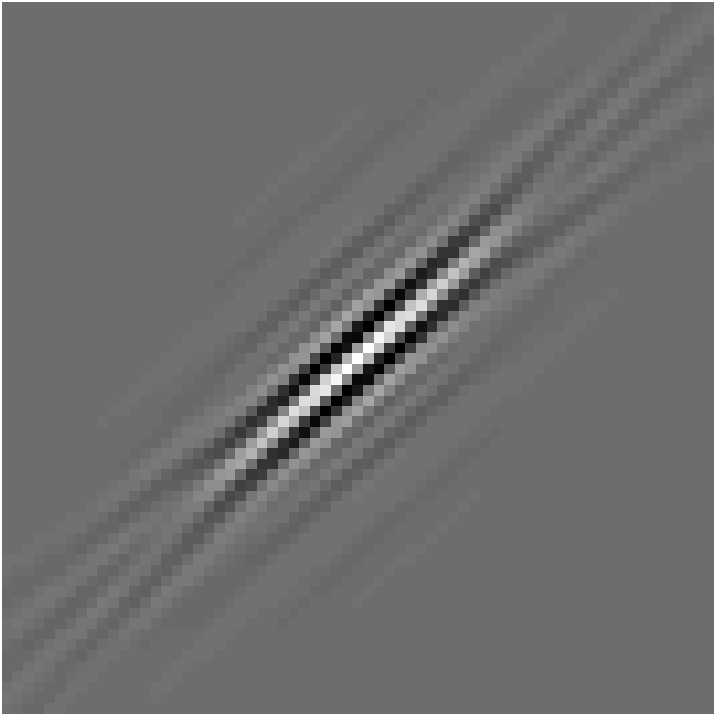
\includegraphics[width=\linewidth]{figures/xp/n4/xp_128x128_sc2_angl1_K3_S3_node4_target.pdf}
\caption{Target $\y$}
\end{subfigure}
\begin{subfigure}[b]{0.49\linewidth}\centering
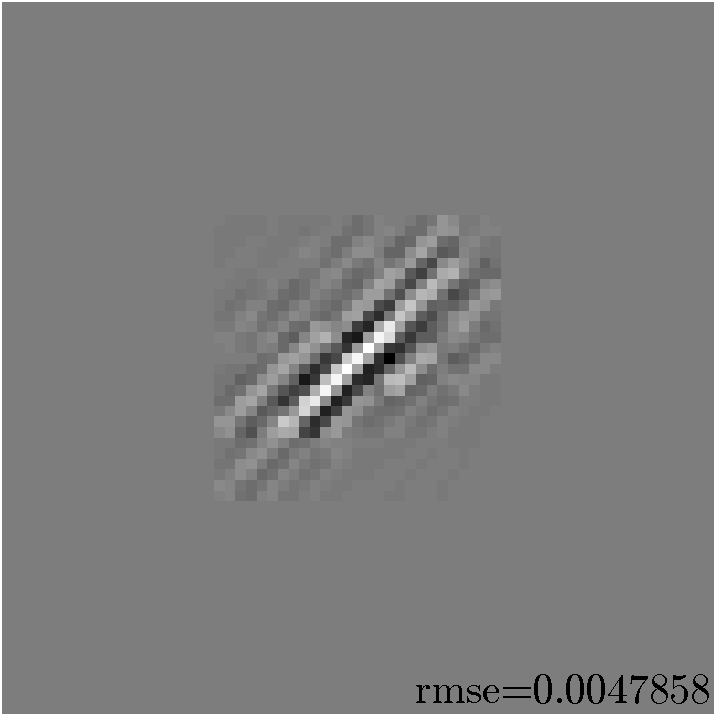
\includegraphics[width=\linewidth]{figures/xp/n4/xp_128x128_sc2_angl1_K3_S3_node4_approx.pdf}
\caption{Approximation $\D\x$} \label{fig_gain_n4_approx}
\end{subfigure}
\begin{subfigure}[b]{0.49\linewidth}\centering
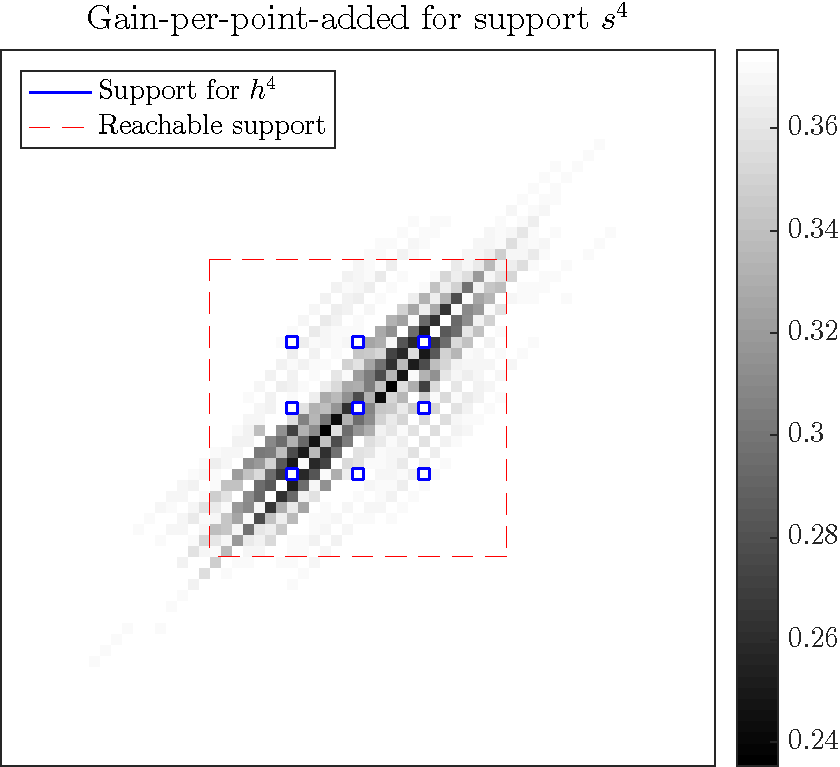
\includegraphics[width=\linewidth]{figures/xp/n4/xp_128x128_sc2_angl1_K3_S3_node4_objmatrix.pdf}
\caption{Gain-per-added-point for $\s^4$}
\end{subfigure}
\begin{subfigure}[b]{0.49\linewidth}\centering
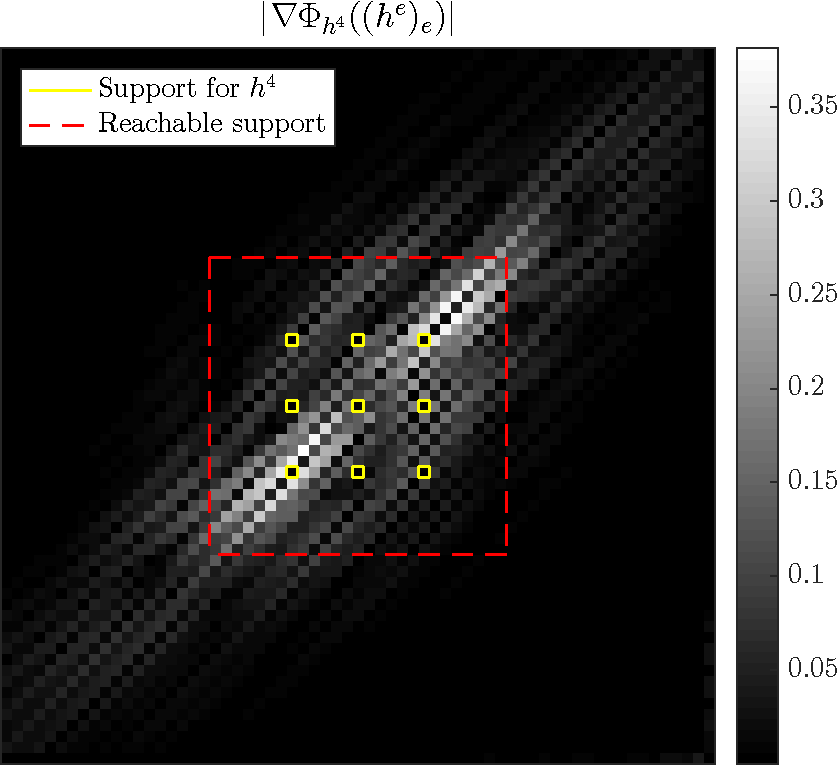
\includegraphics[width=\linewidth]{figures/xp/n4/xp_128x128_sc2_angl1_K3_S3_node4_partgrad4.pdf}
\caption{Partial gradient w.r.t $\h^4$}
\end{subfigure}
\begin{subfigure}[b]{0.49\linewidth}\centering
\includegraphics[width=\linewidth]{figures/xp/n4/xp_128x128_sc2_angl1_K3_S3_node4_objmatrix_bestvalues.pdf}
\caption{Best values of above figure}
\end{subfigure}
\begin{subfigure}[b]{0.49\linewidth}\centering
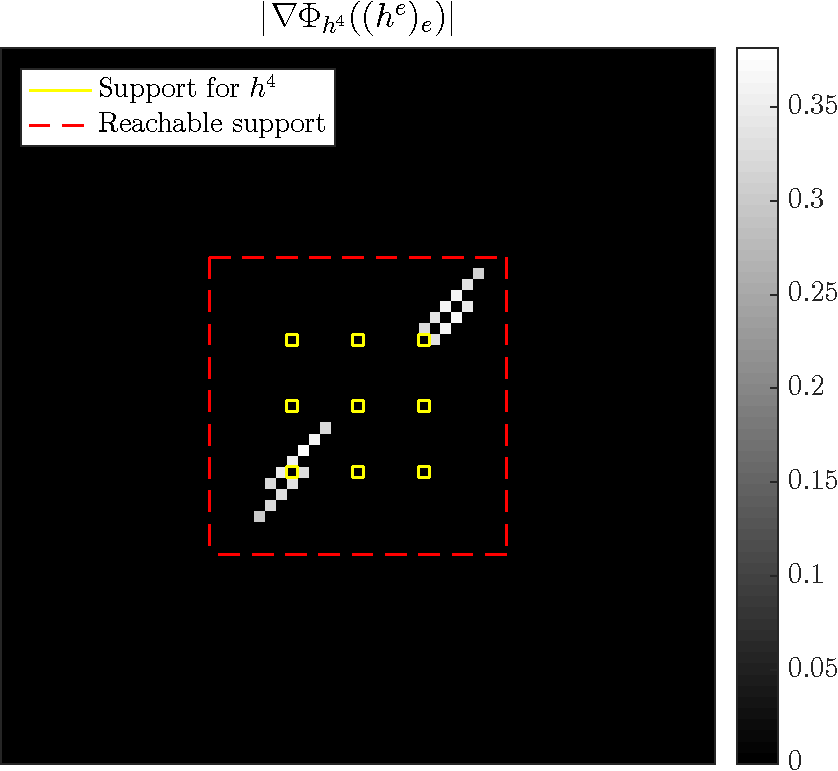
\includegraphics[width=\linewidth]{figures/xp/n4/xp_128x128_sc2_angl1_K3_S3_node4_partgrad4_bestvalues.pdf}
\caption{Best values of above figure}
\end{subfigure}
\end{subfigure}
\caption{Gain-per-added-point compared to “full” gradient. The “full” gradient is computed on the converged “common starting point” $\k$ (see \cref{alg_gain_per_added_point}). The gradient and gain-per-added-point maxima are almost at the same place. }\label{fig_gain_n4}
\end{figure}

\Cref{fig_gain_n4} compares (c) the gain-per-added-point of $\s^4$ to (d) the absolute value of the partial gradient w.r.t $\h^4$ after a convergence of \eqref{eq_ftl}. It is interesting to see that they share the same direction and shape. After selecting 20 of their best values in (e) and (f), we notice that they almost match, which reinforces our hypothesis that the gradient could give the right information for widening supports.

Note the null gradient values on the points of the support (small squares); with respect to those nine points, the necessary condition for optimality is met. However, the rest of the gradient is not null, meaning we are on a suboptimal solution.

\begin{figure}[!ht]\centering
	\begin{subfigure}[b]{0.24\linewidth}\centering
	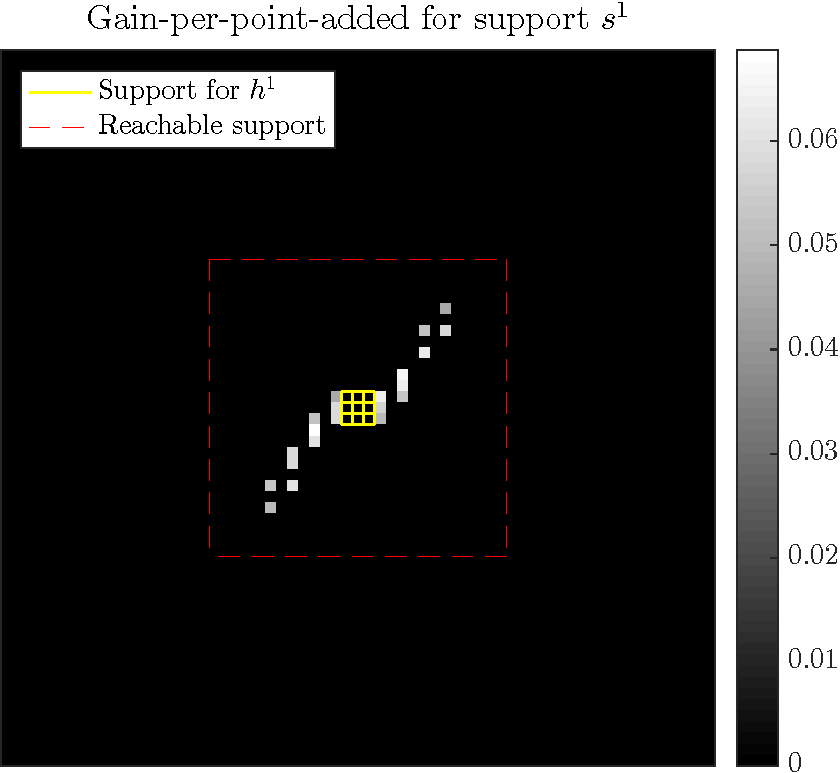
\includegraphics[width=\linewidth]{figures/xp/n1/xp_128x128_sc2_angl1_K3_S3_node1_objmatrix_bestvalues.pdf}
	\caption{$\s^1$ gain}
	\end{subfigure}
	\begin{subfigure}[b]{0.24\linewidth}\centering
	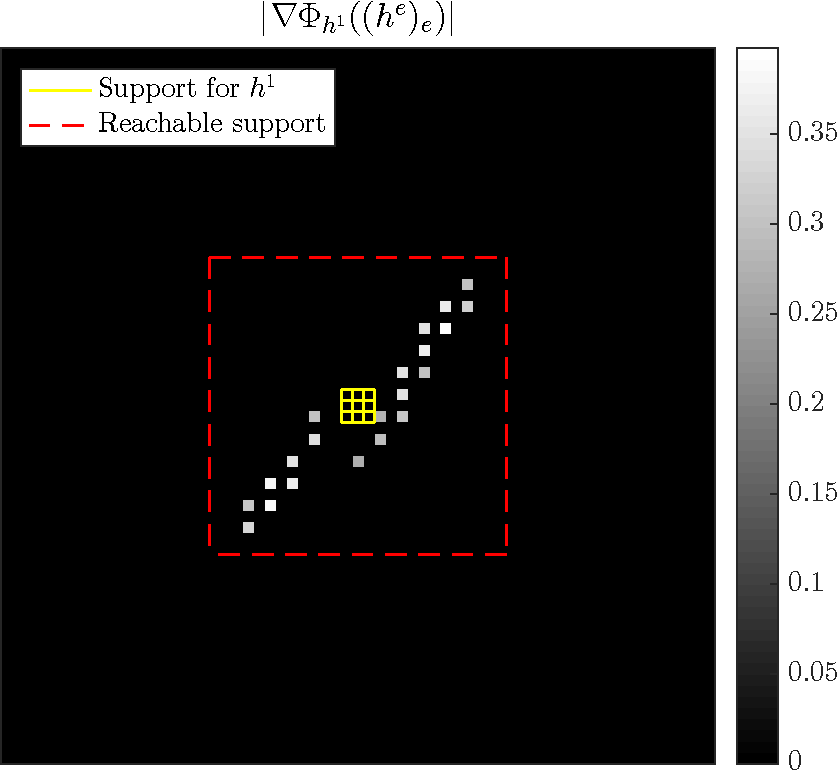
\includegraphics[width=\linewidth]{figures/xp/n1/xp_128x128_sc2_angl1_K3_S3_node1_partgrad1_bestvalues.pdf}
	\caption{$\h^1$ gradient}
	\end{subfigure}
	\begin{subfigure}[b]{0.24\linewidth}\centering
	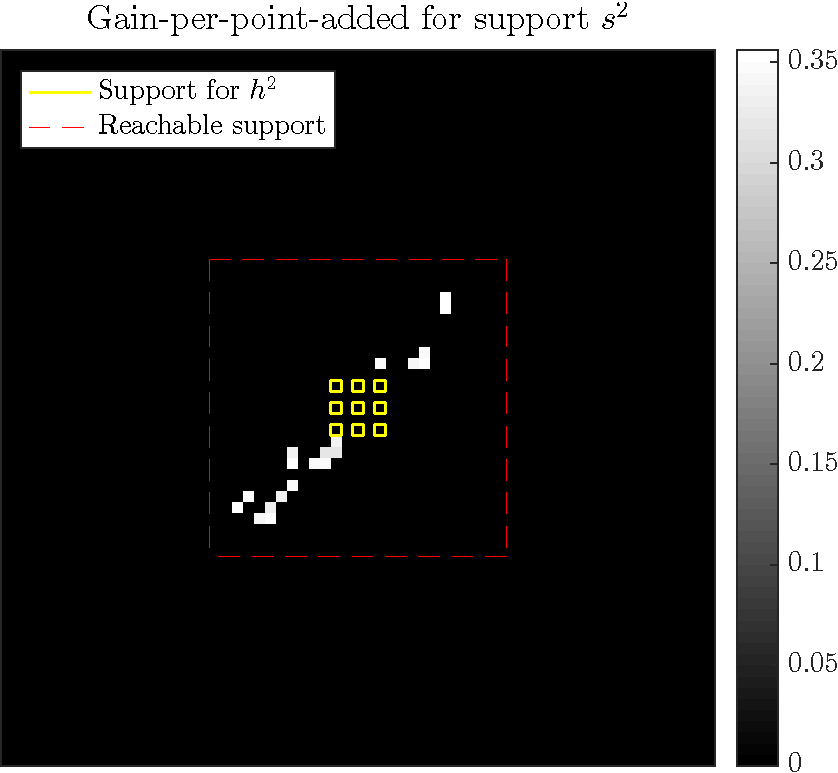
\includegraphics[width=\linewidth]{figures/xp/n2/xp_128x128_sc2_angl1_K3_S3_node2_objmatrix_bestvalues.pdf}
	\caption{$\s^2$ gain}
	\end{subfigure}
	\begin{subfigure}[b]{0.24\linewidth}\centering
	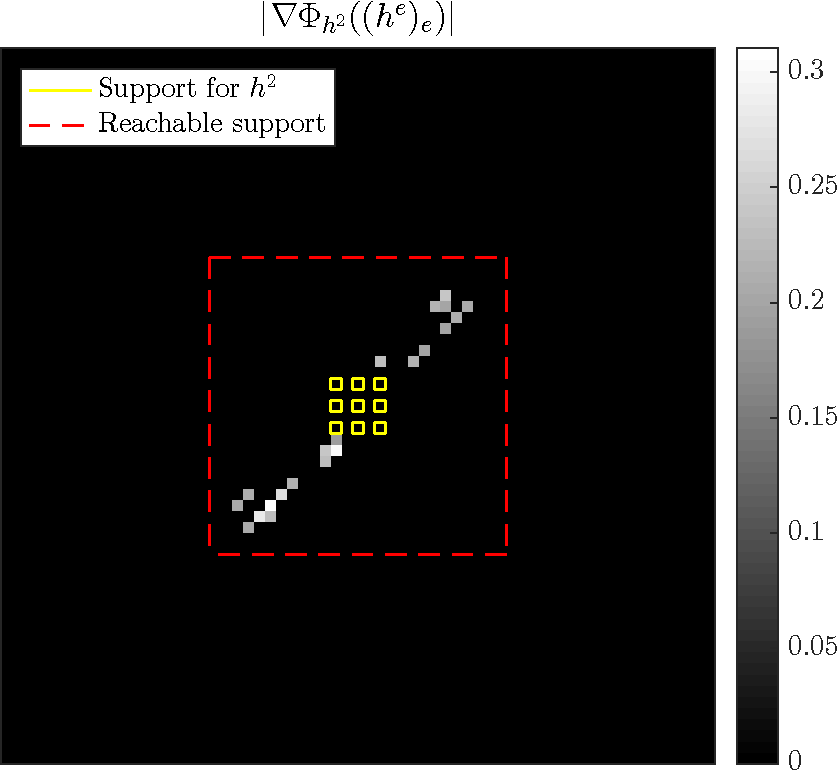
\includegraphics[width=\linewidth]{figures/xp/n2/xp_128x128_sc2_angl1_K3_S3_node2_partgrad2_bestvalues.pdf}
	\caption{$\h^2$ gradient}
	\end{subfigure}
\caption{Two other edges (1 and 2) for experiment in \cref{fig_gain_n4}. The image $\y$ and its approximation $\D\x$ are identical to \cref{fig_gain_n4}.}\label{fig_gain_n1_n2}
\end{figure}

\Cref{fig_gain_n1_n2} does the same comparison for two other kernels of the same tree (it is the same experiment). Whatever the kernel, the best values of the gradient seem to follow the same shape as the gain-per-added-point matrix. 

\begin{figure}[!ht]\centering
	\begin{subfigure}[b]{0.22\textwidth}\centering
	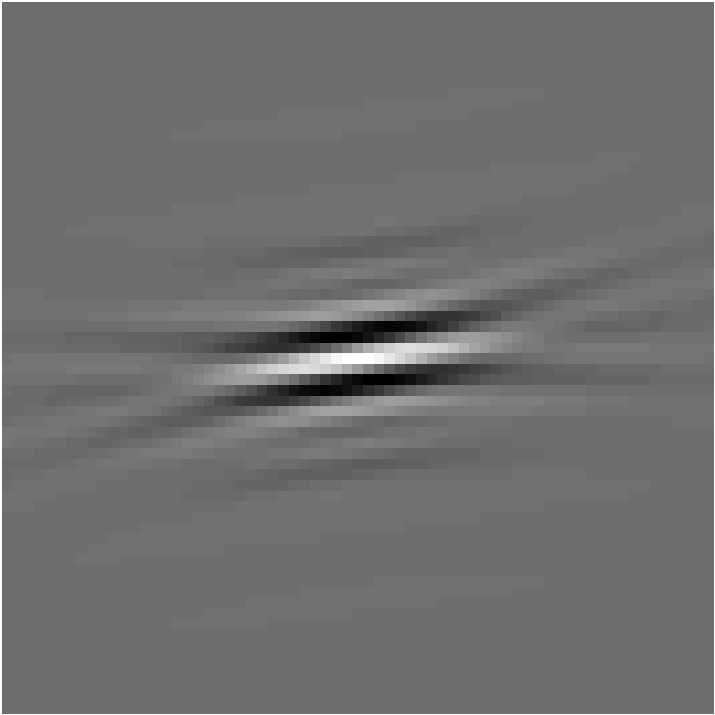
\includegraphics[width=\textwidth]{figures/xp/tilted_n4/xp_128x128_sc2_angl4_K3_S3_node4_target.pdf}
	\caption{Target $\y$}
	\end{subfigure}
	\begin{subfigure}[b]{0.22\textwidth}\centering
	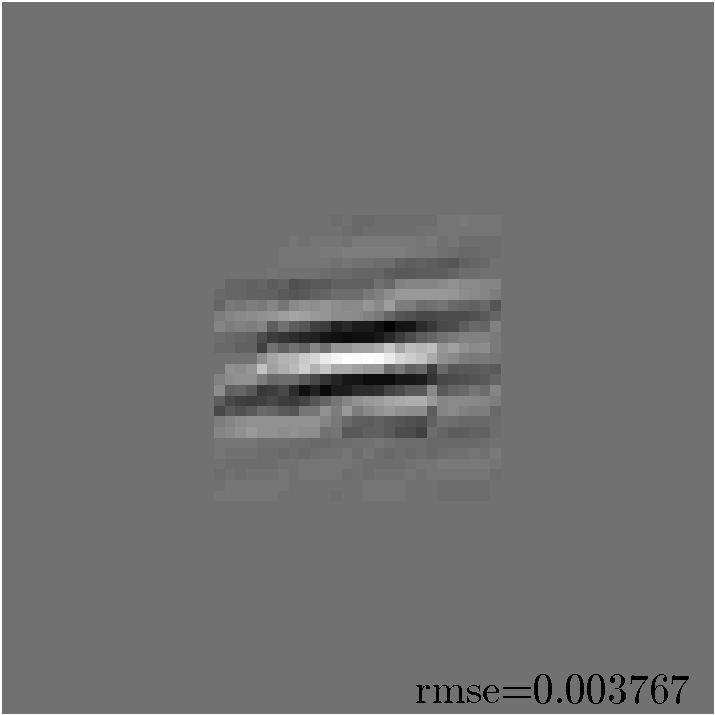
\includegraphics[width=\textwidth]{figures/xp/tilted_n4/xp_128x128_sc2_angl4_K3_S3_node4_approx.pdf}
	\caption{Approx. $\D\x$}
	\end{subfigure}
	\begin{subfigure}[b]{0.26\textwidth}\centering
	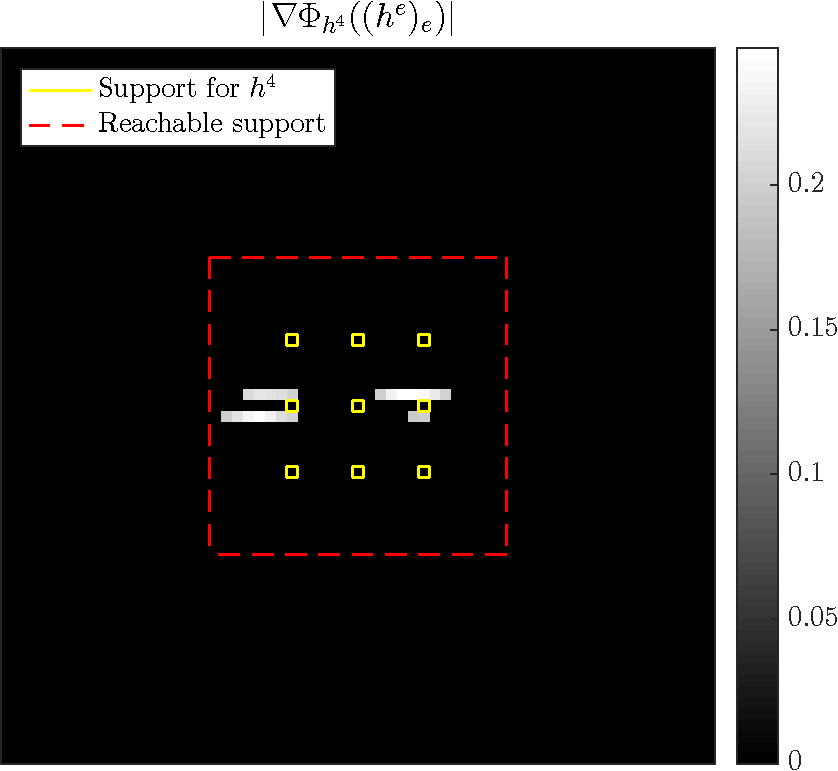
\includegraphics[width=\textwidth]{figures/xp/tilted_n4/xp_128x128_sc2_angl4_K3_S3_node4_partgrad4_bestvalues.pdf}
	\caption{$\s^4$ gain}
	\end{subfigure}
	\begin{subfigure}[b]{0.26\textwidth}\centering
	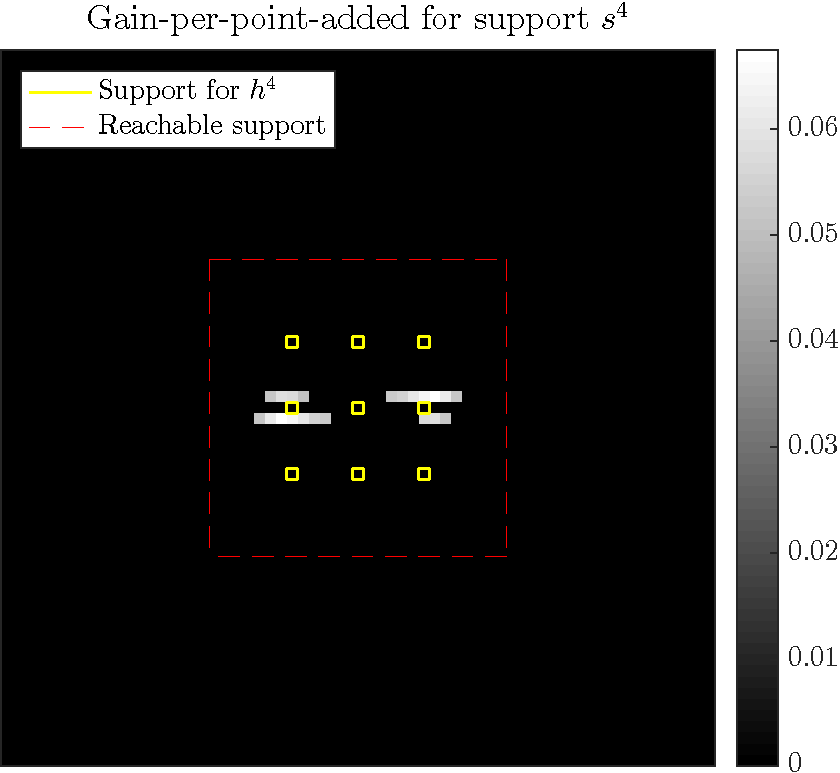
\includegraphics[width=\textwidth]{figures/xp/tilted_n4/xp_128x128_sc2_angl4_K3_S3_node4_objmatrix_bestvalues.pdf}
	\caption{$\h^4$ gradient}
	\end{subfigure}
\caption{Trying a different $\y$.}\label{fig_gain_tilted_n4}
\end{figure}

Finally, \cref{fig_gain_tilted_n4} presents the same experiment but with a different atom (this time, a curvelet with a different angle). And as for the two previous figures, the gradient matches the gain-per-added-point.

\subsection{Visual gain when adding an element}

\begin{figure}[!ht]\centering
\begin{subfigure}[b]{0.32\linewidth}\centering
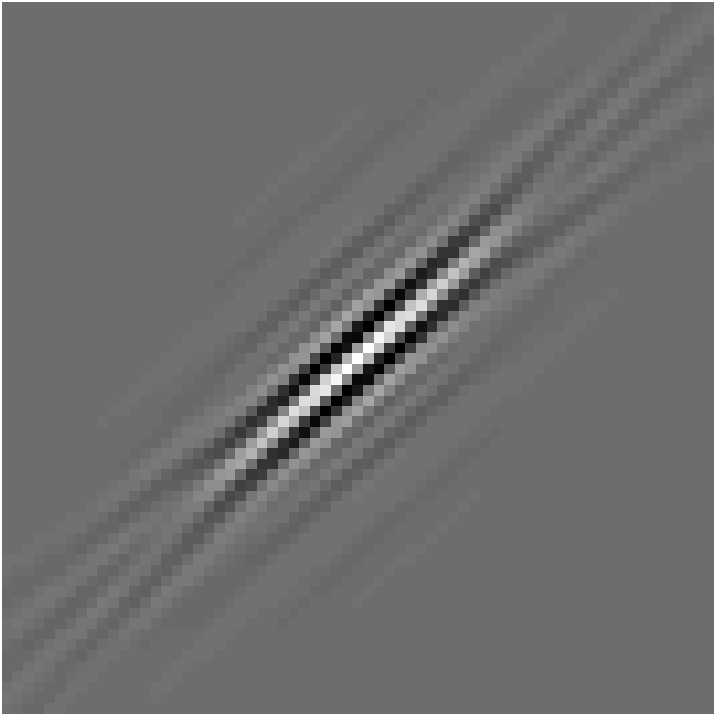
\includegraphics[width=\linewidth]{figures/before_after/xp_128x128_sc2_angl1_K3_S3_node4before_target.pdf}
	\caption{Target image}
\end{subfigure}
\begin{subfigure}[b]{0.32\linewidth}\centering
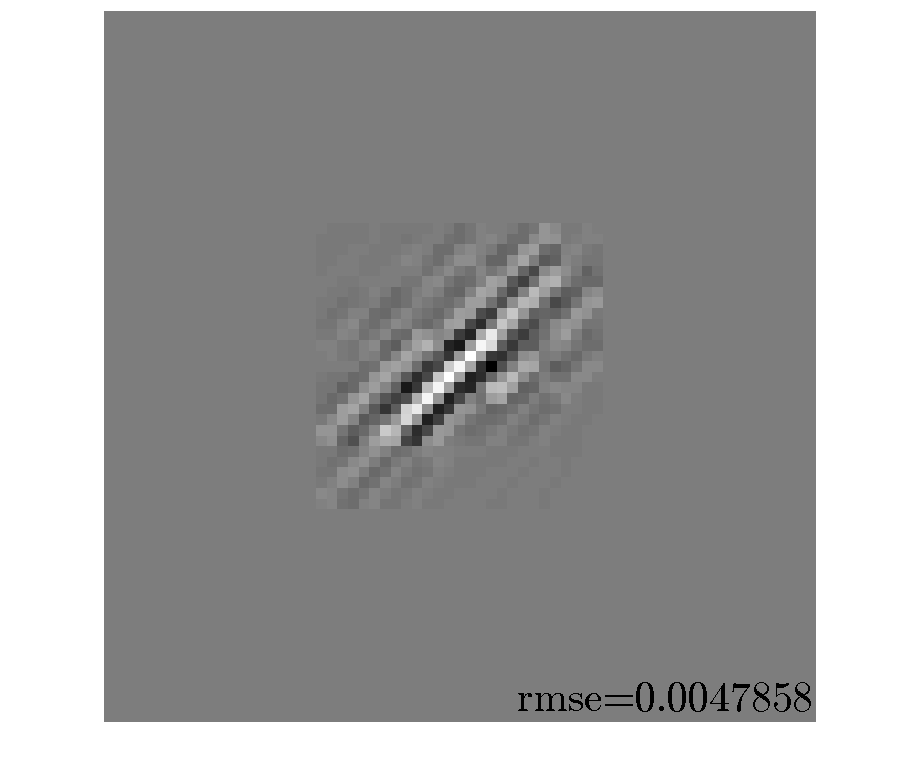
\includegraphics[width=\linewidth]{figures/before_after/xp_128x128_sc2_angl1_K3_S3_node4before_approx.pdf}
\caption{Before adding}
\end{subfigure}
\begin{subfigure}[b]{0.32\linewidth}\centering
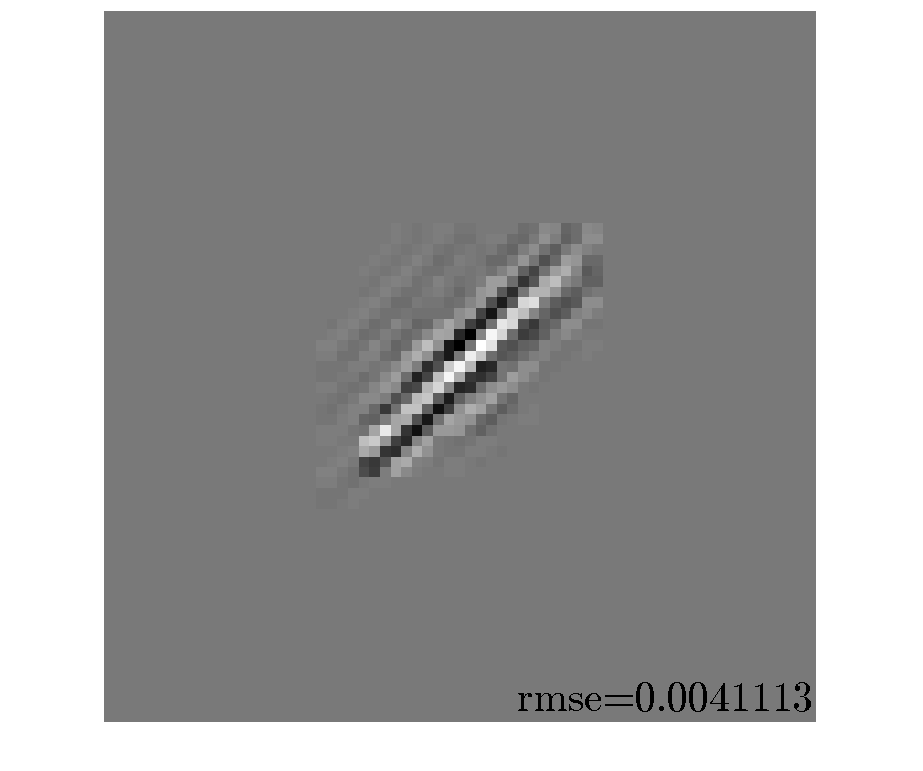
\includegraphics[width=\linewidth]{figures/before_after/xp_128x128_sc2_angl1_K3_S3_node4after_approx.pdf}
\caption{After adding}
\end{subfigure}
\begin{subfigure}[b]{0.32\linewidth}\centering
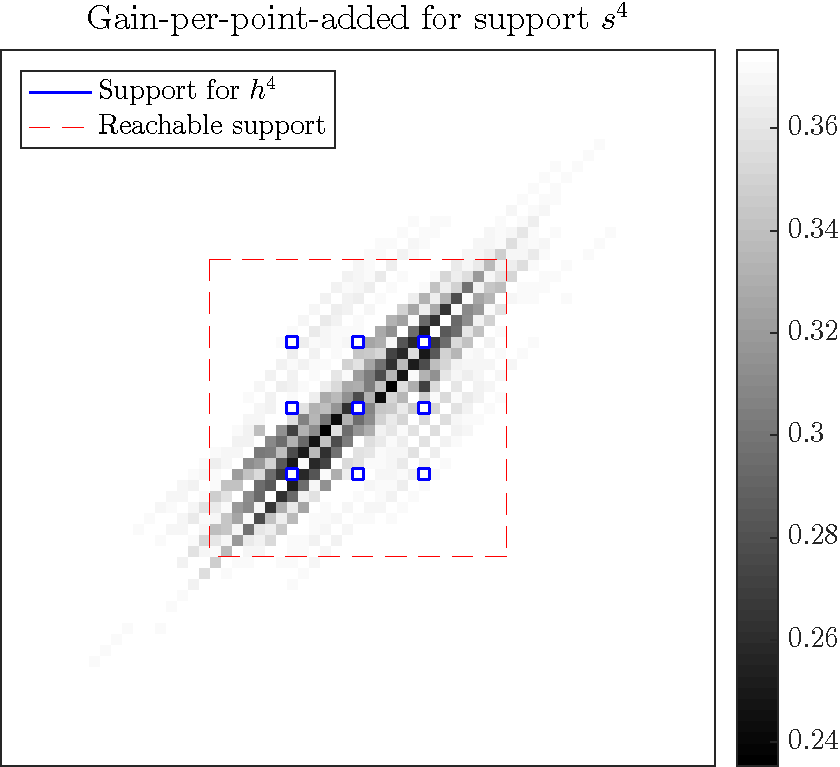
\includegraphics[width=\linewidth]{figures/before_after/xp_128x128_sc2_angl1_K3_S3_node4before_objmatrix.pdf}
\caption{Gain-per-added-point} \label{fig_gain_matrix}
\end{subfigure}
\begin{subfigure}[b]{0.32\linewidth}\centering
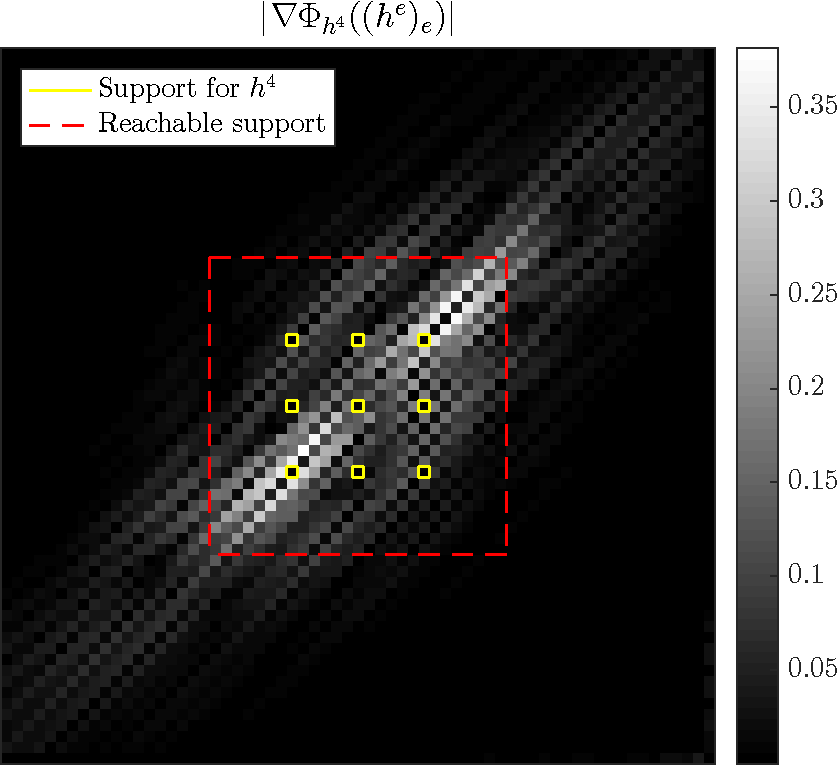
\includegraphics[width=\linewidth]{figures/before_after/xp_128x128_sc2_angl1_K3_S3_node4before_partgrad4.pdf}
\caption{Gradient before} \label{fig_grad_before}
\end{subfigure}
\begin{subfigure}[b]{0.32\linewidth}\centering
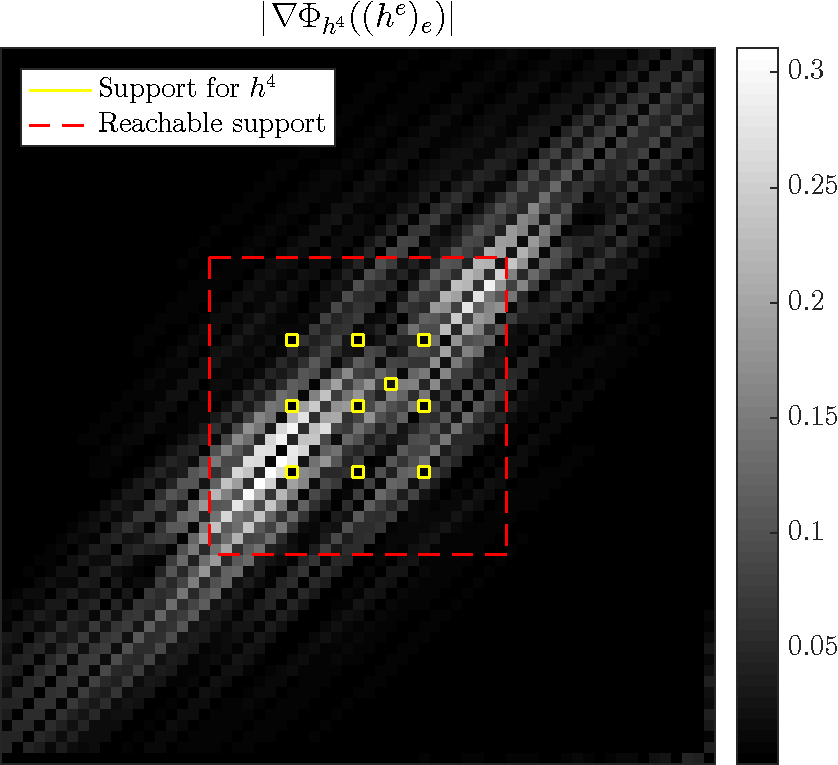
\includegraphics[width=\linewidth]{figures/before_after/xp_128x128_sc2_angl1_K3_S3_node4after_partgrad4.pdf}
\caption{Gradient after} \label{fig_grad_after}
\end{subfigure}
\begin{subfigure}[b]{0.32\linewidth}\centering
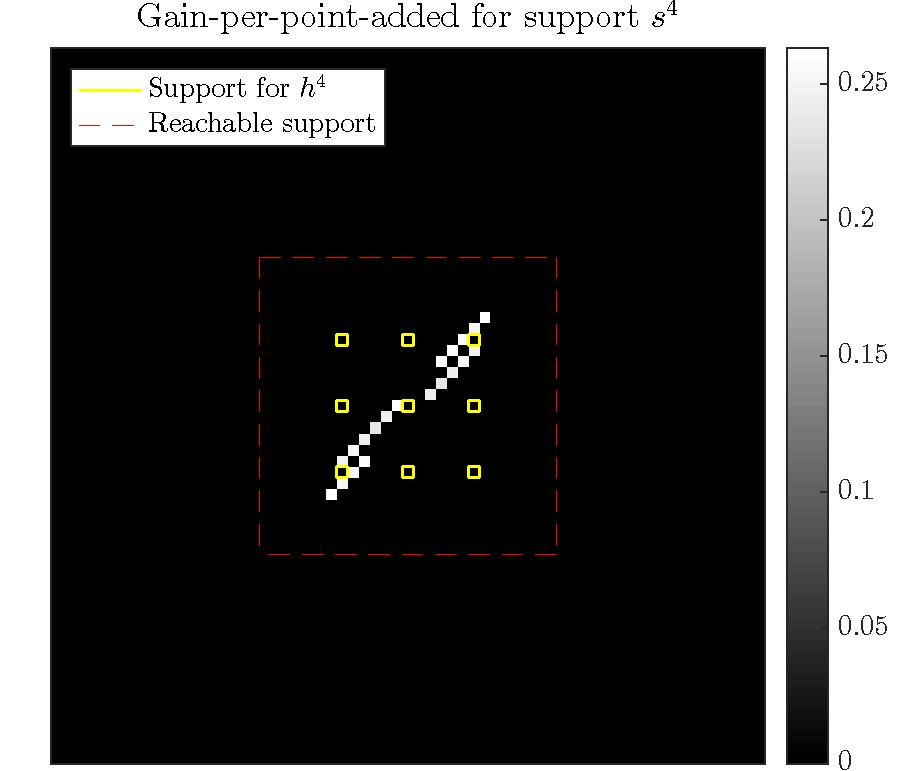
\includegraphics[width=\linewidth]{figures/before_after/xp_128x128_sc2_angl1_K3_S3_node4before_objmatrix_bestvalues.pdf}
\caption{Best values of \ref{fig_gain_matrix}}
\end{subfigure}
\begin{subfigure}[b]{0.32\linewidth}\centering
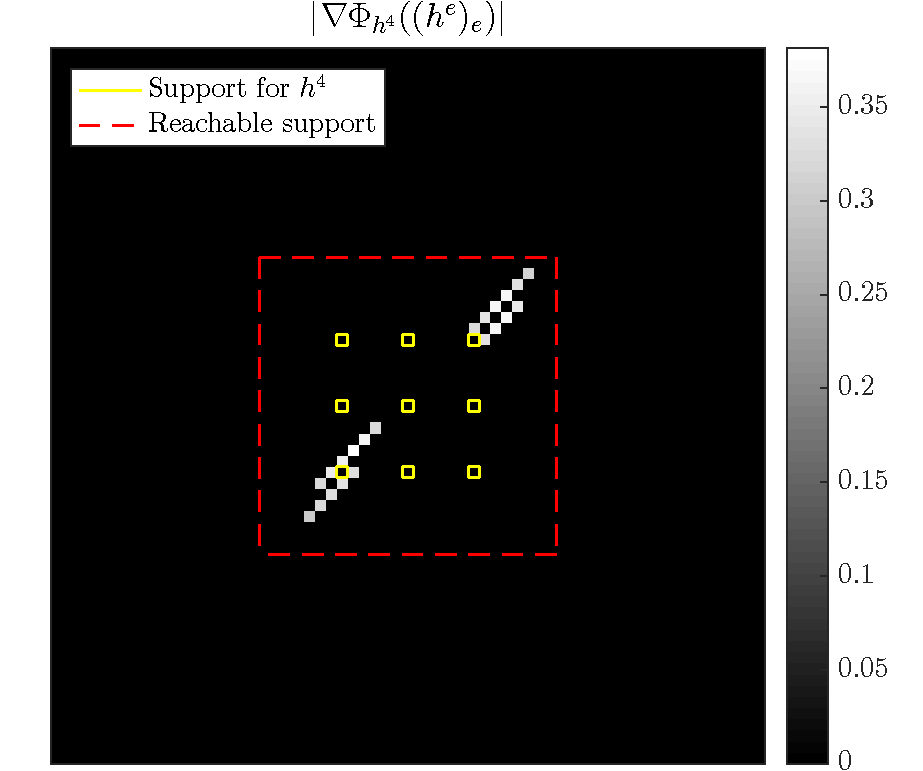
\includegraphics[width=\linewidth]{figures/before_after/xp_128x128_sc2_angl1_K3_S3_node4before_partgrad4_bestvalues.pdf}
\caption{Best values of \ref{fig_grad_before}}
\end{subfigure}
\begin{subfigure}[b]{0.32\linewidth}\centering
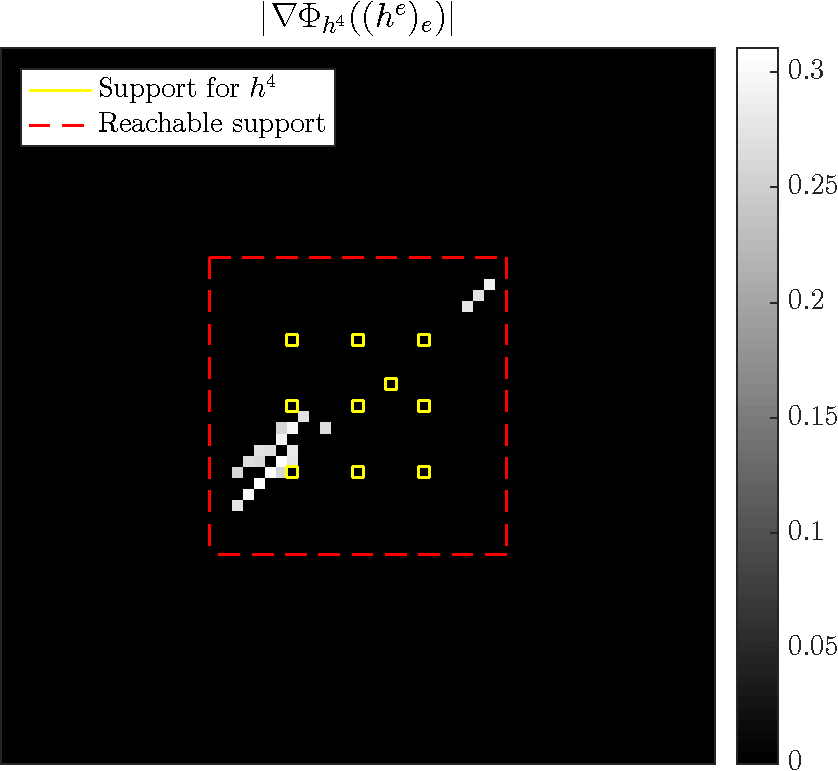
\includegraphics[width=\linewidth]{figures/before_after/xp_128x128_sc2_angl1_K3_S3_node4after_partgrad4_bestvalues.pdf}
\caption{Best values of \ref{fig_grad_after}}
\end{subfigure}
\caption{Effect of adding one point to the support $\s^4$. The “before” tree is a converged solution of \ac{PALMTREE}. The “after” tree has been added a point where the gain-per-added-point was maximal.}\label{fig_before_after_adding}
\end{figure}

The experiment shown in \cref{fig_before_after_adding} is based on the results of \cref{fig_gain_n4_approx}, where figures (a,b,d,e,g,h) are the same as the previous experiment. The figures (c,j,i) show what  happens if we add the minimum point of gain-per-added-point to $\s^4$ and continue the minimization. We note that the approximation (c) looks visually closer to the target image; the RMSE is decreased by -16\% (lower is better).

We also observe that when adding a point to the support (materialized by the \nth{10} small square), the highest gradient values “shift” to the south-west. Adding a point to the support has an effect on every surrounding points.

\subsection{Adding elements before the convergence of \ac{PALMTREE}} \label{sec_add_before_converged}

At \cref{alg_omppalmtree_ftl} of \cref{alg_omppalmtree}, we do a full minimization, i.e. it stops as soon as \ac{PALMTREE} has converged. Because the minimization takes a lot of time, it was tempting to try adding elements every few iterations of \ac{PALMTREE} instead of waiting until it converges.

The \cref{fig_gain_n4} has shown that the “full” gradient could be satisfactorily used for adding elements to the support $s$, provided that \cref{alg_palmtree} at \cref{alg_omppalmtree_ftl} has converged. Would the gradient still give a valid information on a not-yet converged solution $\k$ of \ac{PALMTREE}, for example after 5 iterations?

\begin{figure}[!ht]\centering
\begin{subfigure}[b]{0.49\linewidth}\centering
\includegraphics[width=\linewidth]{figures/xp_grad_iterations/xp_128x128_sc2_angl1_K3_S3_node4_objmatrix_bestvalues.pdf}
\caption{Gain-per-added-point matrix}
\end{subfigure}
\begin{subfigure}[b]{0.49\linewidth}\centering
	\begin{subfigure}[b]{0.49\linewidth}\centering
	\includegraphics[width=\linewidth]{figures/xp_grad_iterations/xp_128x128_sc2_angl1_K3_S3_node4_iter1_partgrad4_bestvalues.pdf}
	\caption{Grad. iter. 1}
	\end{subfigure}
	\begin{subfigure}[b]{0.49\linewidth}\centering
	\includegraphics[width=\linewidth]{figures/xp_grad_iterations/xp_128x128_sc2_angl1_K3_S3_node4_iter8_partgrad4_bestvalues.pdf}
	\caption{Grad. iter. 8}
	\end{subfigure}
	\begin{subfigure}[b]{0.49\linewidth}\centering
	\includegraphics[width=\linewidth]{figures/xp_grad_iterations/xp_128x128_sc2_angl1_K3_S3_node4_iter20_partgrad4_bestvalues.pdf}
	\caption{Grad. iter. 20}
	\end{subfigure}
	\begin{subfigure}[b]{0.49\linewidth}\centering
	\includegraphics[width=\linewidth]{figures/xp_grad_iterations/xp_128x128_sc2_angl1_K3_S3_node4_iter200_partgrad4_bestvalues.pdf}
	\caption{Grad. iter. 200}
	\end{subfigure}
\end{subfigure}
\caption{Is the gradient giving the same information depending on the iteration of \ac{PALMTREE}? This is the same experiment as \cref{fig_gain_n4}. Only the best values are displayed.}\label{fig_iter_gain_vs_grad}
\end{figure}

\Cref{fig_iter_gain_vs_grad} compares the best values of gain-per-added-point to gradient snapshots taken during the minimization. This is reassuring: whatever the iteration, the gradient best values stay close to the gain-per-added-point best values. We may conclude that adding elements every few iterations of \ac{PALMTREE} works.


\section{Learning the supports}
%This section presents some results regarding 

\subsection{Learning supports by only adding}
After having shown that the gradient would give a good indication on which support elements should be added, we tried learning the support $\s$ using the \cref{alg_omppalmtree}. According to the conclusions of \cref{sec_add_before_converged} that indicates that the convergence of \ac{PALMTREE} is not mandatory before adding an element, we modified the \ac{PALMTREE} algorithm so that it stops every $t$ iterations.

In \cref{fig_variable_support}, the initial supports are simply centered Diracs; every $t=5$ iterations, one element is added where the gradient is the greatest, up to 36 elements. The experiment converges after about 200 iterations.

The resulting approximation is encouraging with a relative RMSE decrease of -76\% compared to the approximation in \cref{fig_gain_n4}.

\begin{figure}[!ht]\centering
\begin{subfigure}[b]{0.3\textwidth}\centering
	\begin{subfigure}[b]{1\textwidth}\centering
	\includegraphics[width=\textwidth]{figures/variable_support/xp_128x128_sc2_angl1_K3_S3_node4_variable_target.pdf}
	\caption{Image $\y$}
	\end{subfigure}
	\begin{subfigure}[b]{1\textwidth}\centering
	\includegraphics[width=\textwidth]{figures/variable_support/xp_128x128_sc2_angl1_K3_S3_node4_variable_approx.pdf}
	\caption{Approximation $\D\x$}
	\end{subfigure}
\end{subfigure}
\begin{subfigure}[b]{0.3\textwidth}\centering
\includegraphics[width=0.47\textwidth]{figures/variable_support/support.pdf}
\caption{Supports $\s_e$}
\end{subfigure}
\caption{Learning the support (adding elements only). Starting from simple Diracs, the best element (using greatest gradient) is added to one of the supports every 5 iterations, up to 36 elements (same number as the fixed support in \cref{fig_gain_n4}).} \label{fig_variable_support}
\end{figure}

\section{Conclusions and perspectives}

\todo[inline]{PALMTREE should be able to handle multiple images}
\todo[inline]{test PALMTREE on a real dictionary learning example (with sparse coding step)}


\clearpage
\addcontentsline{toc}{chapter}{Appendix}
\appendix

\chapter{Miscellaneous}


\section{Link between \gls{treemodel} and dictionary matrix}\label{sec_matrix_vs_tree} % $\bm{D} in \section{} bugs

Figure \ref{fig_block_circular} outlines the relation between the tree and the matrix forms of $\D\x$ in the \gls{treemodel}. The dictionary $\D$ can be written using the notation
$$\D = \begin{bmatrix}C^5 & C^6\end{bmatrix} \begin{bmatrix}C^1 & C^2 & 0 & 0 \\0 & 0 & C^3 & C^4\end{bmatrix}$$
with $C^i$ the block-circular matrix for $\h^i$; it represents the final convolution $\h^{*l}*\x^l$ when using matrices.

\begin{figure}[!ht] \centering
\begin{subfigure}[b]{0.30\textwidth}\centering
\includegraphics[width=\textwidth]{figures/pov-tree.pdf}
\caption{Convolutional tree}
\end{subfigure}
\begin{subfigure}[b]{0.69\textwidth}\centering
\includegraphics[width=\textwidth]{figures/pov-matrix.pdf}
\caption{Best values of above figure}
\end{subfigure}
\caption{This figure shows how to go from the tree defined by its kernels $(\h^e)_{e \in \E}$ to a matrix $\D$} \label{fig_block_circular}
\end{figure}

\clearpage

\section{Detail of the \ac{KSVD} algorithm} \label{sec_ksvd_detail}
\begin{algorithm}
    \caption{\ac{KSVD} (K-Singular Value Decomposition) algorithm for \eqref{eq_dl_ksvd}} \label{alg_ksvd}
  \begin{algorithmic}[1]
    \Input signal samples $\y_i$ of dimension $N$ forming the $S$ columns of $\Y$
    \Output dictionary $\D$ of dim. $K \times N$ with $K \gg N$
    \State \textbf{Initialization} Initialize $\D$ such that every column is $l^2$ normalized
    \While{not converged}
	\State For each image $\y_i$, solve \Comment{\textbf{Sparse Coding step}} \label{alg_ksvd_sparse_coding}
		\begin{align*}
			\quad \min_{\x_i}~ & \lVert \y_i-\D\x_i\rVert^2 \quad \text{s.t.}~ \lVert \x_i \rVert_0 \le \gamma
		\end{align*}
	\State $\D^{old} = \D$
	\State For each atom $\d_k^{old}$ of $\D^{old}$, \Comment{\textbf{Dictionary Update step}}\label{alg_ksvd_dict_update}
	\begin{enumerate}[leftmargin=15mm,label=(\alph*)]
		\item find the images $\y_i$ that use the atom $\d_k^{old}$, meaning $\x_i^k \ne 0$ \label{item_atom_used}
		\item compute the error matrix associated to this atom,
		\begin{align*}
			\bm{E}_k = \Y-\sum_{i\ne k} \x_i^T\d_i^{old}
		\end{align*}
		\item keep only columns of $\bm{E}_k$ found in \cref{item_atom_used}
		\item Apply SVD decomposition $\bm{E}_k - \bm{U} \Delta V^T$. The first column of $\bm{U}$ becomes the new $\d_k$. $\x_k$ is updated using the first column of $\bm{V}$ multiplied by $\Delta(1,1)$ (highest eigenvalue)
	\end{enumerate}
    \EndWhile
  \end{algorithmic}
\end{algorithm}

\clearpage

\section{Why is sparse coding used for denoising?}

The figure \ref{sparse_reduce_noise} shows a noisy signal $\y$ living in a high-dimensional subspace of dimension $N$ and defined by
$$\y=\hat{\y} + \bm{b}$$
with $\bm{b}$ following a centered Gaussian distribution $\mathcal{N}(0,\sigma^2I)$ and $\hat{\y}$ the noiseless signal. We see that the distance $||\bm{b}||$ is always smaller than the projected distance.

This is because the variance in the $N$ dimensional space can be written as
\begin{align*}
\sigma^2(\bm{b}) =& \mathbb{E}\left[\lVert \bm{b}-\mathbb{E}(\bm{b}) \rVert^2 \right]\\
=& \mathbb{E}\left(\lVert \bm{b} \rVert^2 \right)\\
=& \mathbb{E}\left(\sum^N_{i=1} b_i^2 \right)\\
\shortintertext{And as the variance is also $\sigma^2(\bm{b})= \frac{1}{N}\left(\sum_{i=1}^N b_i^2 \right) - \mathbb{E}(\bm{b})^2$, it becomes}
=& \mathbb{E} \left(N\sigma^2(\bm{b}) + N\mathbb{E}(\bm{b})^2\right)\\
=& N \mathbb{E} \left(\sigma^2(\bm{b})\right)\\
=& ... \\
=& \frac{1}{N}\lVert \bm{b} \rVert^2
\end{align*}\todo{Ask for help}
which gives 
$$ \lVert \bm{b} \rVert = \sigma\sqrt{N} $$
When projected onto the $k$ dimensional space, the noise deviation becomes
$$\lVert \bm{b} \rVert = \sigma\sqrt{k} $$
which is much better than the previous distance, provided that $k \ll N$. 

\begin{figure}[!ht]\centering
\includegraphics[width=0.4\textwidth]{figures/sparse-reduce-noise.pdf}
\caption{When projected onto a lower dimensional space, the standard deviation of the additive Gaussian noise $\bm{b} \sim \mathcal{N}(0,\sigma^2I)$ will be greatly reduced if $k \ll N$. The sparser the representation the better the denoising. \label{sparse_reduce_noise}}
\end{figure}

\clearpage

\section{Why $\F(\widetilde{A}) = \F(A)^*$}
\todo[inline]{This is a meaningless proof; I’ll remove it}
\begin{align*}
(\widehat{\widetilde{A}})_{m,n} =& \sum_{k=1}^M \sum_{l=1}^N \widetilde{A}_{k,l} e^{-2i\pi (k\frac{m}{M}+l \frac{n}{N})}\\
=& \sum_{k=1}^M \sum_{l=1}^N A_{-k,-l} e^{-2i\pi (k\frac{m}{M}+l \frac{n}{N})}\\
\shortintertext{By changing variables $k’=-k$ and $l’=-l$, we get:}
=& \sum_{k’=-M}^{-1} \sum_{l’=-N}^{-1} A_{k’,l’} e^{2i\pi (k’\frac{m}{M}+l’ \frac{n}{N})}
\shortintertext{And thanks to the $(M,N)$ periodicity of $A$, which means that $A_{i,j}=A_{i+kM,j+lN}$, $\forall (k,l) \in \mathbb{N}^2$, letting us with:}
=& \sum_{k'=-M}^{-1} \sum_{l'=-N}^{-1} A_{k'+M,l'+N} e^{2i\pi (k'\frac{m}{M}+l' \frac{n}{N})}\\
\shortintertext{With a second change of variables $k''=k'+M$ and $l''=l'+N$:}
=& \sum_{k''=-M+M}^{-1+M} \sum_{l''=-N+N}^{-1+N} A_{k'',l''} e^{2i\pi (k'\frac{m}{M}+l' \frac{n}{N})}\\
=& \sum_{k'=1}^{M} \sum_{l'=1}^{N} A_{k',l'} e^{2i\pi (k'\frac{m}{M}+l' \frac{n}{N})}
\end{align*}\todo{To be continued}

\printglossary
{\let\clearpage\relax \printacronyms}
\addcontentsline{toc}{chapter}{References}\printbibliography[title=References]


\end{document}



